\documentclass[11pt,oneside]{book} % Standard book format with 10pt font

\input{e-ai_tutorial_packages}

%==============================================================================
%
%
%==============================================================================
\begin{document}

%-------------------------------
% Front Matter: Title Page
%-------------------------------
\frontmatter
\begin{titlepage}
	\begin{flushright}
    \includegraphics[width=0.3\textwidth]{images/DWD-Logo_2013.svg.png}
	\end{flushright}

  \centering
  % DWD Logo (ensure the file exists in the working directory)
  %\includegraphics[width=0.4\textwidth]{Deutscherwetterdienst-logo.svg.png}\\[1cm]
	\vspace{4cm}
  
  {\Huge\bfseries Python and Machine Learning for Weather, Climate and Environment \par}
  \vspace{1cm}
  
  {\Large\bfseries Tutorial and Guide\par}
  \vspace{2cm}
  
  {\Large Roland Potthast \par 
	
	with contributions by Stefanie Hollborn, Jan Keller, Thomas Deppisch, Mareike Burba, Matthias Mages, Sarah Heibutzki, Marek Jacob, Florian Prill, Tobias Göcke, Felix Fundel \par}
  \vfill
  {\Large \today\par}
\end{titlepage}

\tableofcontents

\frontmatter
\renewcommand{\thechapter}{\Roman{chapter}}
\renewcommand{\thesection}{\thechapter\Roman{section}} % Removes extra dot

\input{chapters/ch00} % Basic Python, Environments, Modules, Core Language

% Reset numbering after Introduction
\renewcommand{\thechapter}{\arabic{chapter}}
\renewcommand{\thesection}{\arabic{chapter}.\arabic{section}}

%-------------------------------
% Main Matter: Chapters
%-------------------------------
\mainmatter

\addtocontents{toc}{\noindent\hrulefill\vspace{-1.5ex}\par}
\addcontentsline{toc}{chapter}{\textcolor{dwdspecial}{\large Day 1: Python as Workhorse}}

\input{chapters/ch01} % Basic Python, Environments, Modules, Core Language
\input{chapters/ch02} % Jupyter Notebooks, Clouds and Servers
\input{chapters/ch03} % eccodes, netcdf, fields and maps

\addtocontents{toc}{\noindent\hrulefill\vspace{-1.5ex}\par}
\addcontentsline{toc}{chapter}{\textcolor{dwdspecial}{\large Day 2: AI/ML Basic Introduction}}

\input{chapters/ch04} % ML Basics, PyTorch
\input{chapters/ch05} % 
\input{chapters/ch06} % 

\addtocontents{toc}{\noindent\hrulefill\vspace{-1.5ex}\par}
\addcontentsline{toc}{chapter}{\textcolor{dwdspecial}{\large Day 3: LLM RAG, Python Packages, Multi-Modality}}

\input{chapters/ch07} %
\input{chapters/ch08} %
\input{chapters/ch09} %

\addtocontents{toc}{\noindent\hrulefill\vspace{-1.5ex}\par}
\addcontentsline{toc}{chapter}{\textcolor{dwdspecial}{\large Day 4: Diffusion Networks, AI Agents, Feature Detection}}

\chapter{Diffusion and flexible Graph Networks}

%==============================================================================
%
%==============================================================================
\section{Diffusion Networks}

%------------------------------------------------------------------------------
%
%------------------------------------------------------------------------------
\subsection{Introduction}

Diffusion models represent a class of generative neural networks that have recently achieved remarkable success in areas such as image generation (e.g., DALL\textperiodcentered E 2, Stable Diffusion) and molecular design. Their core principle is inspired by physical diffusion processes: transforming data into noise and learning to reverse this process. In this way, diffusion models learn to generate new data samples from pure noise through a learned denoising process.

In the context of weather and climate, diffusion models offer a new paradigm for generative modeling, ensemble forecasting, and uncertainty quantification. Traditional numerical weather prediction (NWP) relies on the integration of physical models forward in time, often facing challenges in representing uncertainty and producing diverse ensemble members. Diffusion models can be used as a complementary or alternative strategy: they learn the statistical structure of weather or climate fields and generate samples that respect these statistics, conditioned on given observations or coarse-resolution forecasts.

This section introduces the core ideas and mathematical framework of diffusion models, with a focus on applications to geophysical data.

%------------------------------------------------------------------------------
%
%------------------------------------------------------------------------------
\subsection{Forward and Reverse Diffusion Processes}

%------------------------------------------------------------------------------
%
%------------------------------------------------------------------------------
\subsubsection{The Forward Process (Adding Noise)}

Let $\mathbf{x}_0 \in \mathbb{R}^d$ be a sample from the true data distribution (e.g., a temperature field, wind vector, or other atmospheric variable on a spatial grid). The forward diffusion process corrupts $\mathbf{x}_0$ over $T$ discrete time steps by gradually adding Gaussian noise, producing a sequence of increasingly noisy samples $\mathbf{x}_1, \dots, \mathbf{x}_T$.

\begin{figure}[htbp]
    \centering
    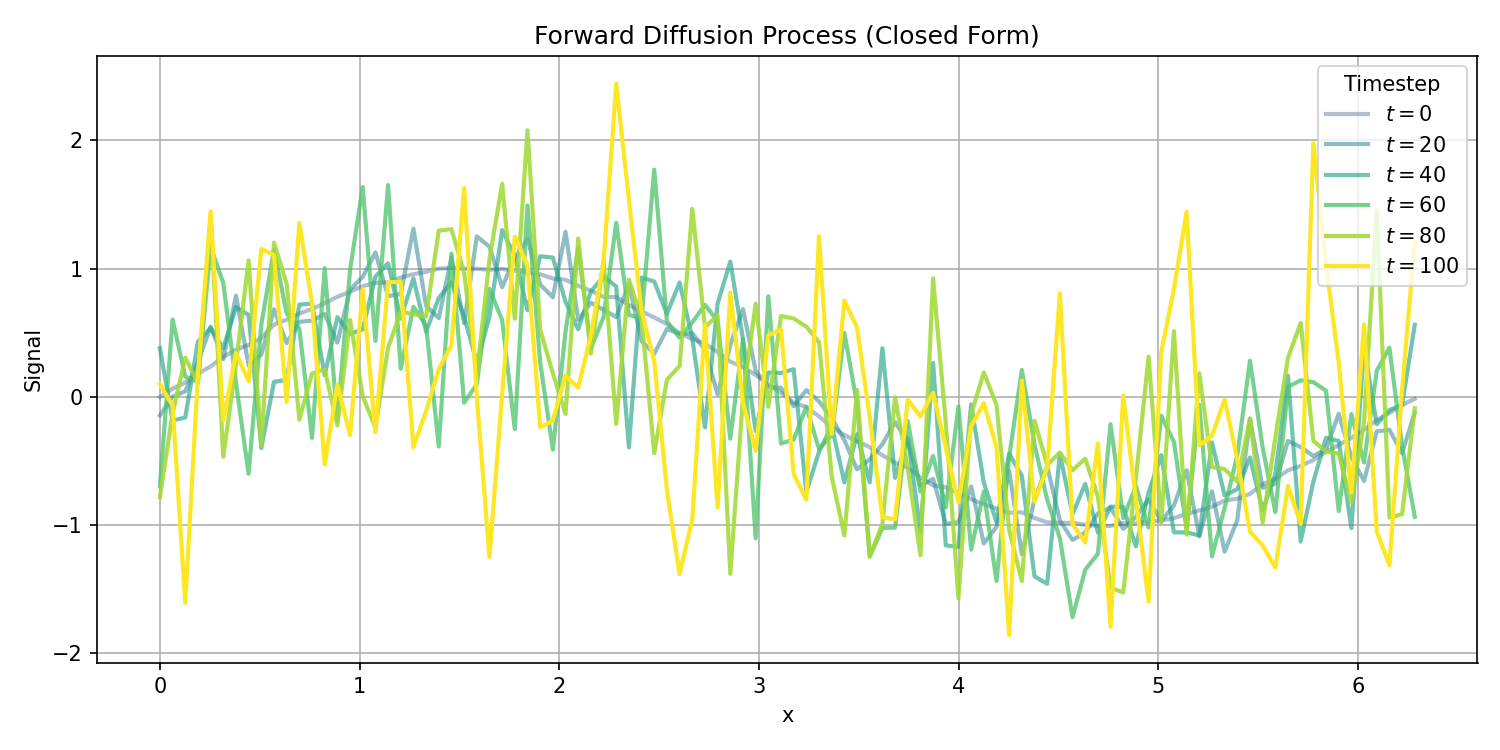
\includegraphics[width=0.9\textwidth]{images/diffusion1.png}
    \caption{
        Forward diffusion process applied to a sine function over 101 steps.
        Every 20th step is shown with increasing transparency and brightness.
        Initially, the signal is clean (\( t=0 \)), and as the diffusion progresses,
        Gaussian noise increasingly dominates the structure. The process is
        governed by a predefined noise schedule using a cumulative variance
        parameter \( \bar{\alpha}_t \), ensuring that \( \mathbf{x}_t \) converges
        toward a standard Gaussian distribution as \( t \rightarrow T \).
    }
    \label{fig:diffusion-forward}
\end{figure}


This process is modeled as a Markov chain:

$$
q(\mathbf{x}_1, \dots, \mathbf{x}_T | \mathbf{x}_0) = \prod_{t=1}^T q(\mathbf{x}_t | \mathbf{x}_{t-1}),
$$

where each transition adds noise as:

$$
q(\mathbf{x}_t | \mathbf{x}_{t-1}) = \mathcal{N}(\mathbf{x}_t; \sqrt{1 - \beta_t} \mathbf{x}_{t-1}, \beta_t \mathbf{I}).
$$
Here, each component in the Gaussian transition
\[
q(\mathbf{x}_t \mid \mathbf{x}_{t-1}) = \mathcal{N}\left(\mathbf{x}_t;\, \sqrt{1 - \beta_t} \, \mathbf{x}_{t-1},\, \beta_t \mathbf{I} \right)
\]
has the following role and dimensional interpretation:
\begin{itemize}
    \item \( \mathbf{x}_t \in \mathbb{R}^d \) is the noisy variable at step \( t \), drawn from the distribution.
    \item The mean of the Gaussian is \( \boldsymbol{\mu}_t = \sqrt{1 - \beta_t} \, \mathbf{x}_{t-1} \in \mathbb{R}^d \), which scales the previous state downward. This reduces the signal amplitude as noise is added, ensuring the data gradually diffuses toward a Gaussian distribution.
    \item The covariance is \( \boldsymbol{\Sigma}_t = \beta_t \mathbf{I} \in \mathbb{R}^{d \times d} \), where \( \mathbf{I} \) is the identity matrix. This defines isotropic Gaussian noise with variance \( \beta_t \) in each dimension.
    \item \( \beta_t \in (0, 1) \) is a predefined noise schedule that increases over time. Small values at early steps retain more structure; larger values at later steps ensure full noise.
\end{itemize}

As \( t \to T \), the distribution of \( \mathbf{x}_t \) converges to the standard normal distribution \( \mathcal{N}(0, \mathbf{I}) \), effectively transforming structured data into pure noise.


As $t \to T$, the sample $\mathbf{x}_T$ approaches pure Gaussian noise: $\mathcal{N}(0, \mathbf{I})$.
This process is fixed and does not involve learning. It provides synthetic training pairs $(\mathbf{x}_t, t, \mathbf{x}_0)$ to train the reverse model.

%------------------------------------------------------------------------------
%
%------------------------------------------------------------------------------
\subsubsection{The Reverse Process (Learning to Denoise)}

The generative aspect of diffusion models lies in the reverse process, which seeks to map noise back to data. This process is defined by:

$$
p_\theta(\mathbf{x}_{0:T}) = p(\mathbf{x}_T) \prod_{t=1}^T p_\theta(\mathbf{x}_{t-1} | \mathbf{x}_t),
$$

where:
\begin{itemize}
\item $p(\mathbf{x}_T) = \mathcal{N}(0, \mathbf{I})$ is the assumed prior distribution (pure noise),
\item $p_\theta(\mathbf{x}_{t-1} | \mathbf{x}_t)$ is the learned denoising distribution parameterized by a neural network.
\end{itemize}

The network predicts a mean $\mu_\theta(\mathbf{x}_t, t)$ and often assumes a fixed variance $\Sigma_t$, resulting in:

$$
p_\theta(\mathbf{x}_{t-1} | \mathbf{x}_t) = \mathcal{N}(\mathbf{x}_{t-1}; \mu_\theta(\mathbf{x}_t, t), \Sigma_t).
$$

The denoising network can be conditioned on additional inputs such as class labels, spatial information, or physical constraints, making it suitable for structured data like weather fields.

%------------------------------------------------------------------------------
%
%------------------------------------------------------------------------------
\subsection{Loss Function and Training}

In the denoising framework used here, the neural network is trained to predict a less noisy version of the input, i.e., an estimate of \( \mathbf{x}_{t-1} \) given the current noisy state \( \mathbf{x}_t \) and conditioning information (e.g., class or weather constraints).

At each training step, we use a sequence of noisy inputs generated from a known clean signal \( \mathbf{x}_0 \), perturbed by Gaussian noise through the forward process. The training loss at each denoising step is given by the mean squared error:

\[
\mathcal{L}_t(\theta) = \mathbb{E}_{\mathbf{x}_{t}, \mathbf{x}_{t-1}} \left[ \left\| \mathbf{x}_{t-1} - f_\theta(\mathbf{x}_t, t, \text{cond}) \right\|^2 \right],
\]

where:
\begin{itemize}
    \item \( \mathbf{x}_t \in \mathbb{R}^d \) is the noisy state at time \( t \),
    \item \( \mathbf{x}_{t-1} \in \mathbb{R}^d \) is the target (previous, less noisy) state,
    \item \( f_\theta(\cdot, t, \text{cond}) \) is the neural network that predicts the denoised state, possibly conditioned on class labels or physical context,
    \item The expectation is taken over randomly sampled timesteps and training examples.
\end{itemize}

The total loss is averaged over all reverse steps from \( t = T \) to \( 1 \). This approach turns denoising into a stepwise regression problem toward the clean signal trajectory, rather than estimating the noise directly as in DDPM.

%------------------------------------------------------------------------------
%
%------------------------------------------------------------------------------
\subsection{Relevance to Weather and Climate}

In weather and climate science, data is high-dimensional, often spatial-temporal, and exhibits strong structure (e.g., physical constraints, correlations, seasonal cycles). Diffusion models are particularly suited to such domains because they:

\begin{itemize}
\item Learn \textbf{nonlinear distributions} of full fields (e.g., 2m temperature, geopotential height),
\item Allow \textbf{conditional generation}, e.g., generating high-resolution forecasts conditioned on coarse-resolution inputs,
\item Support \textbf{stochastic generation}, producing diverse ensemble members,
\item Can be guided or constrained by physical priors or observations.
\end{itemize}

Recent applications include:
\begin{itemize}
\item Generating ensemble weather forecast members,
\item Downscaling global climate model (GCM) outputs,
\item Imputing missing observations (gap-filling),
\item Emulating expensive simulation models.
\end{itemize}

By learning to sample plausible geophysical states from noise while respecting physical structure, diffusion models represent a promising approach for next-generation generative systems in atmospheric science.

%------------------------------------------------------------------------------
%
%------------------------------------------------------------------------------
\begin{figure}[htbp]
    \centering
    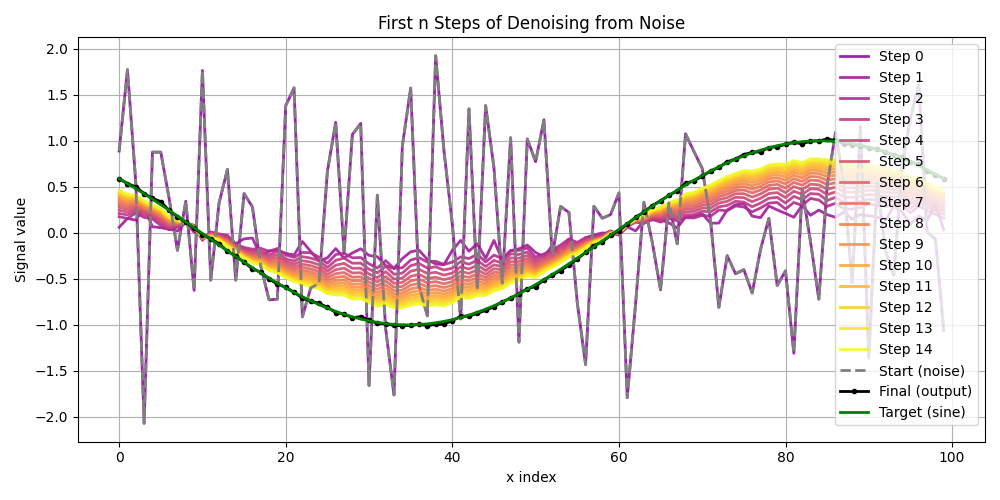
\includegraphics[width=0.9\textwidth]{images/diffusion_denoising.png}
    \caption{%
        The first 15 steps of the denoising process, starting from white noise (dashed gray).
        Colored curves represent the intermediate states.
        The model quickly adjusts toward the structure of the target sine (green),
        with the final output (black dots) nearly matching it.
    }
    \label{fig:diffusion_denoising}
\end{figure}



\subsection{A Minimal Diffusion Denoising Example}

To demonstrate the principle of diffusion models in a simple and interpretable setting, we construct a minimal 1D example: starting from white noise, a neural network learns to iteratively denoise it toward a target sine curve. We use PyTorch to define and train a small denoising network that learns this reconstruction process in a class-conditional setup.

%------------------------------------------------------------------------------
%
%------------------------------------------------------------------------------
\paragraph{Step 1: Configuration and Target Signal.} We define the sine wave classes, select one target curve, and generate the corresponding label as a one-hot vector.

\begin{codeonly}{Setup Example for Diffusion Network}
import torch
import torch.nn as nn
import torch.optim as optim
import matplotlib.pyplot as plt

# --- Config ---
n_points = 100
n_steps = 50
noise_std = 0.2
class_idx = 2  # Select sine class 0 to 4

# --- Generate sine waves ---
x = torch.linspace(0, 2 * torch.pi, n_points)
phases = torch.arange(5) * (2 * torch.pi / 5)
sine_set = torch.stack([torch.sin(x + p) for p in phases])
x_target = sine_set[class_idx].unsqueeze(0)  # shape [1, n_points]
label = torch.nn.functional.one_hot(torch.tensor([class_idx]), num_classes=5).float()
\end{codeonly}

This sets up our clean signal \( \mathbf{x}_0 \) and class information to be used throughout training and inference.

%------------------------------------------------------------------------------
%
%------------------------------------------------------------------------------
\paragraph{Step 2: Define the Denoising Network.} We now define a small MLP that takes as input the noisy signal and the class label (concatenated) and outputs a denoised signal of the same shape.

\begin{codeonly}{Network for Diffusion Inversion}
# --- Model ---
class DenoiseMLP(nn.Module):
    def __init__(self, n_points, n_classes):
        super().__init__()
        self.net = nn.Sequential(
            nn.Linear(n_points + n_classes, 128),
            nn.ReLU(),
            nn.Linear(128, 128),
            nn.ReLU(),
            nn.Linear(128, n_points)
        )
    def forward(self, x, label):
        return self.net(torch.cat([x, label], dim=1))

model = DenoiseMLP(n_points, n_classes=5)
\end{codeonly}

This architecture is deliberately small to keep training fast and interpretable. The model learns a mapping from noisy versions of the signal to cleaner versions at earlier diffusion steps.

%------------------------------------------------------------------------------
%
%------------------------------------------------------------------------------
\paragraph{Step 3: Training the Denoising Model.} The training process simulates a forward diffusion process by adding Gaussian noise to the clean signal in small increments, then teaches the model to reverse this process step by step. We use a simple mean squared error (MSE) loss to train the model to predict the less-noisy signal at the previous step.

\begin{codeonly}{Optimizer and Noise Generator}
optimizer = optim.Adam(model.parameters(), lr=1e-3)
loss_fn = nn.MSELoss()

# Add progressive noise
def add_noise_sequence(x0, n_steps, noise_std):
    x = x0.clone()
    trajectory = [x]
    for _ in range(n_steps):
        x = x + (noise_std / n_steps) * torch.randn_like(x)
        trajectory.append(x)
    return trajectory
\end{codeonly}

The function \texttt{add\_noise\_sequence} returns a list of noisy versions \( \mathbf{x}_t \) starting from the clean signal \( \mathbf{x}_0 \). Each step adds a small amount of Gaussian noise.

The training loop samples a noisy trajectory and trains the model to denoise from \( \mathbf{x}_t \) to \( \mathbf{x}_{t-1} \), starting from the noisiest point and moving backwards:

\begin{codeonly}{Diffusion Network Training Loop}
for epoch in range(1001):
    noisy_traj = add_noise_sequence(x_target, n_steps, noise_std)
    loss = 0.0
    for t in reversed(range(1, len(noisy_traj))):
        x_in = noisy_traj[t]
        x_out = noisy_traj[t-1]
        x_pred = model(x_in, label)
        loss += loss_fn(x_pred, x_out)
    loss /= n_steps
    optimizer.zero_grad()
    loss.backward()
    optimizer.step()
    if epoch % 100 == 0:
        print(f"Epoch {epoch}: Loss = {loss.item():.6f}")
\end{codeonly}

The model is trained on one fixed sine class, identified by its one-hot label. The loss accumulates over all denoising steps and is averaged before each optimization step. This process teaches the model to reverse the noisy trajectory — one step at a time — and eventually generate a clean sine signal when starting from white noise.

%------------------------------------------------------------------------------
%
%------------------------------------------------------------------------------
\paragraph{Step 4: Reverse Sampling and Visualization}

After training, we use the model as an iterative denoiser: starting from white noise, we repeatedly apply the learned function to reduce noise and guide the signal toward a sine-like structure. This mimics the reverse trajectory of a diffusion process.

\begin{codeonly}{Denoise from White Noise}
# --- Reverse from noise ---
with torch.no_grad():
    x = torch.randn_like(x_target)
    x_start = x.clone()
    traj = [x.squeeze().numpy()]
    for _ in range(n_steps):
        x = model(x, label)
        traj.append(x.squeeze().numpy())
\end{codeonly}

The variable \texttt{traj} stores each intermediate signal. To observe how the denoising unfolds, we visualize the first few steps of the reconstruction process.

\begin{codeonly}{}
# --- Plot first 15 steps + start, final, target ---
import numpy as np
plt.figure(figsize=(10, 5))

steps_to_plot = list(range(0, 15))  # show early progress
colors = plt.cm.plasma(np.linspace(0.3, 1.0, len(steps_to_plot)))

for i, t in enumerate(steps_to_plot):
    plt.plot(traj[t], color=colors[i], alpha=0.9, linewidth=2, label=f"Step {t}")

# Add clearly labeled curves
plt.plot(x_start.squeeze().numpy(), 'gray', linestyle='dashed', linewidth=2, label="Start (noise)")
plt.plot(traj[-1], 'k.', linestyle='-', linewidth=2, label="Final (output)")
plt.plot(x_target.squeeze().numpy(), 'g', linestyle='-', linewidth=2, label="Target (sine)")

plt.title("First n Steps of Denoising from Noise")
plt.xlabel("x index")
plt.ylabel("Signal value")
plt.legend(loc="upper right")
plt.grid(True)
plt.tight_layout()
plt.savefig("diffusion_denoising.png")
plt.show()
\end{codeonly}

The resulting figure (see Figure~\ref{fig:diffusion_denoising}) shows the progressive alignment of the noisy signal toward the clean sine curve.

%------------------------------------------------------------------------------
%
%------------------------------------------------------------------------------
\subsection{Generating Functions from White Noise Using Conditional Diffusion}

In many physical systems, outputs are structured signals — for example, 1D fields like temperature profiles or time-series measurements. These are influenced by both stochastic variability and contextual constraints (e.g., location, boundary conditions, or categories). 

In this section, we explore how diffusion models can generate such signals starting from white noise and guided by a conditioning input — here, a class index that selects one of several sine wave types. This basic idea generalizes to more complex applications, such as generating spatial weather fields from forecasts or even from text prompts.

%------------------------------------------------------------------------------
\subsubsection*{Target Functions: Shifted Sine Waves}

We define \( n_\text{classes} \) shifted sine curves:
\[
s_k(x) = \sin\left(x + \frac{2\pi k}{n_\text{classes}}\right), \quad k = 0, \dots, n_\text{classes} - 1,
\]
sampled on a fixed grid. Each class represents a different target signal.

%------------------------------------------------------------------------------
\subsubsection*{Training the Reverse Process}

The model is trained to denoise progressively. We begin from a clean sine wave \( x_0 \), add noise step-by-step to generate a trajectory \( x_0, x_1, ..., x_T \), and train the model to learn the reverse steps.

Each step of the model takes a noisy signal \( x_t \) and a one-hot encoded class label \( \mathbf{y} \), and predicts the cleaner \( x_{t-1} \). The total loss accumulates the mean squared error across all reverse steps:

\begin{codeonly}{training loop with class-conditioned denoising}
optimizer = optim.Adam(model.parameters(), lr=0.001)
mse_loss = nn.MSELoss()

for epoch in range(601):
    idx = torch.randint(0, n_classes, (batch_size,))
    x_clean = sine_set[idx]
    labels = torch.nn.functional.one_hot(idx, num_classes=n_classes).float()

    x_t = x_clean.clone()
    trajectory = [x_t.clone()]
    for _ in range(n_steps):
        x_t = add_noise_step(x_t, noise_std / n_steps)
        trajectory.append(x_t.clone())

    loss = 0.0
    for step in reversed(range(1, n_steps + 1)):
        x_input = trajectory[step]
        x_target = trajectory[step - 1]
        x_input_with_label = torch.cat([x_input, labels], dim=1)
        x_pred = model(x_input_with_label)

        loss_denoise = mse_loss(x_pred, x_target)
        target_template = labels @ sine_set
        loss_template = mse_loss(x_pred, target_template)
        cos = nn.CosineSimilarity(dim=1)
        loss_cos = 1 - cos(x_pred, target_template).mean()
        loss_align = mse_loss(x_pred, x_clean) if step == 1 else 0.0

        loss += loss_denoise + 2 * loss_template + 0.2 * loss_cos

    loss /= n_steps
    optimizer.zero_grad()
    loss.backward()
    optimizer.step()
\end{codeonly}

%------------------------------------------------------------------------------
\subsubsection*{Generating a Function from Noise}

After training, we can generate a signal starting from white noise. The only input to the model is a class label — for example, the instruction ``give me the curve for class 2.'' The model then iteratively denoises the signal.

\begin{codeonly}{sampling one function from white noise}
x = torch.randn(1, n_points)
label = torch.nn.functional.one_hot(torch.tensor([class_idx]), num_classes=n_classes).float()

for _ in range(n_steps):
    x_input = torch.cat([x, label], dim=1)
    x = amplify * model(x_input)
\end{codeonly}

%------------------------------------------------------------------------------
\subsubsection*{Visualization and Results}

Figure~\ref{fig:sample-overlay} shows multiple generated functions for different class labels, compared to the reference sine curves. Despite starting from pure noise, the output converges to class-consistent functions.

\begin{figure}[h]
\centering
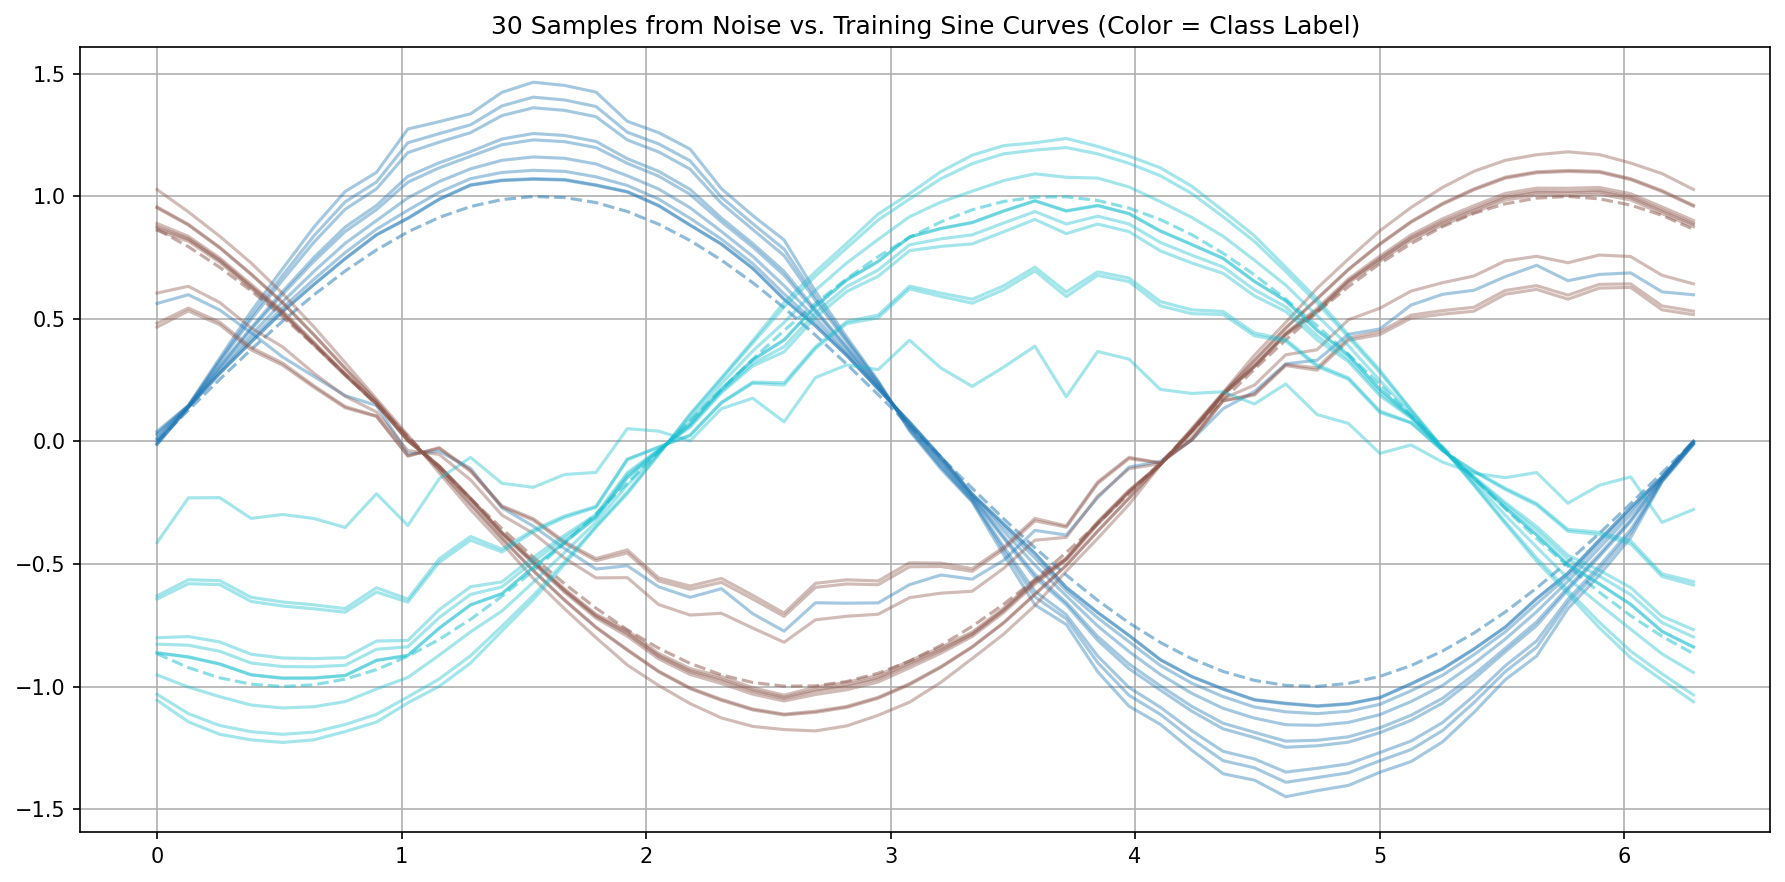
\includegraphics[width=\textwidth]{images/samples_vs_sines_conditioned.png}
\caption{Samples generated from white noise and guided by class label. Colored lines show generated samples, dashed lines the target sine functions.}
\label{fig:sample-overlay}
\end{figure}

To visualize how structure emerges, we also track full denoising trajectories. In each subplot of Figure~\ref{fig:step-by-step}, the signal starts as noise and evolves step-by-step toward the final shape. The gray curve is the ground-truth sine.

\begin{figure}[h]
\centering
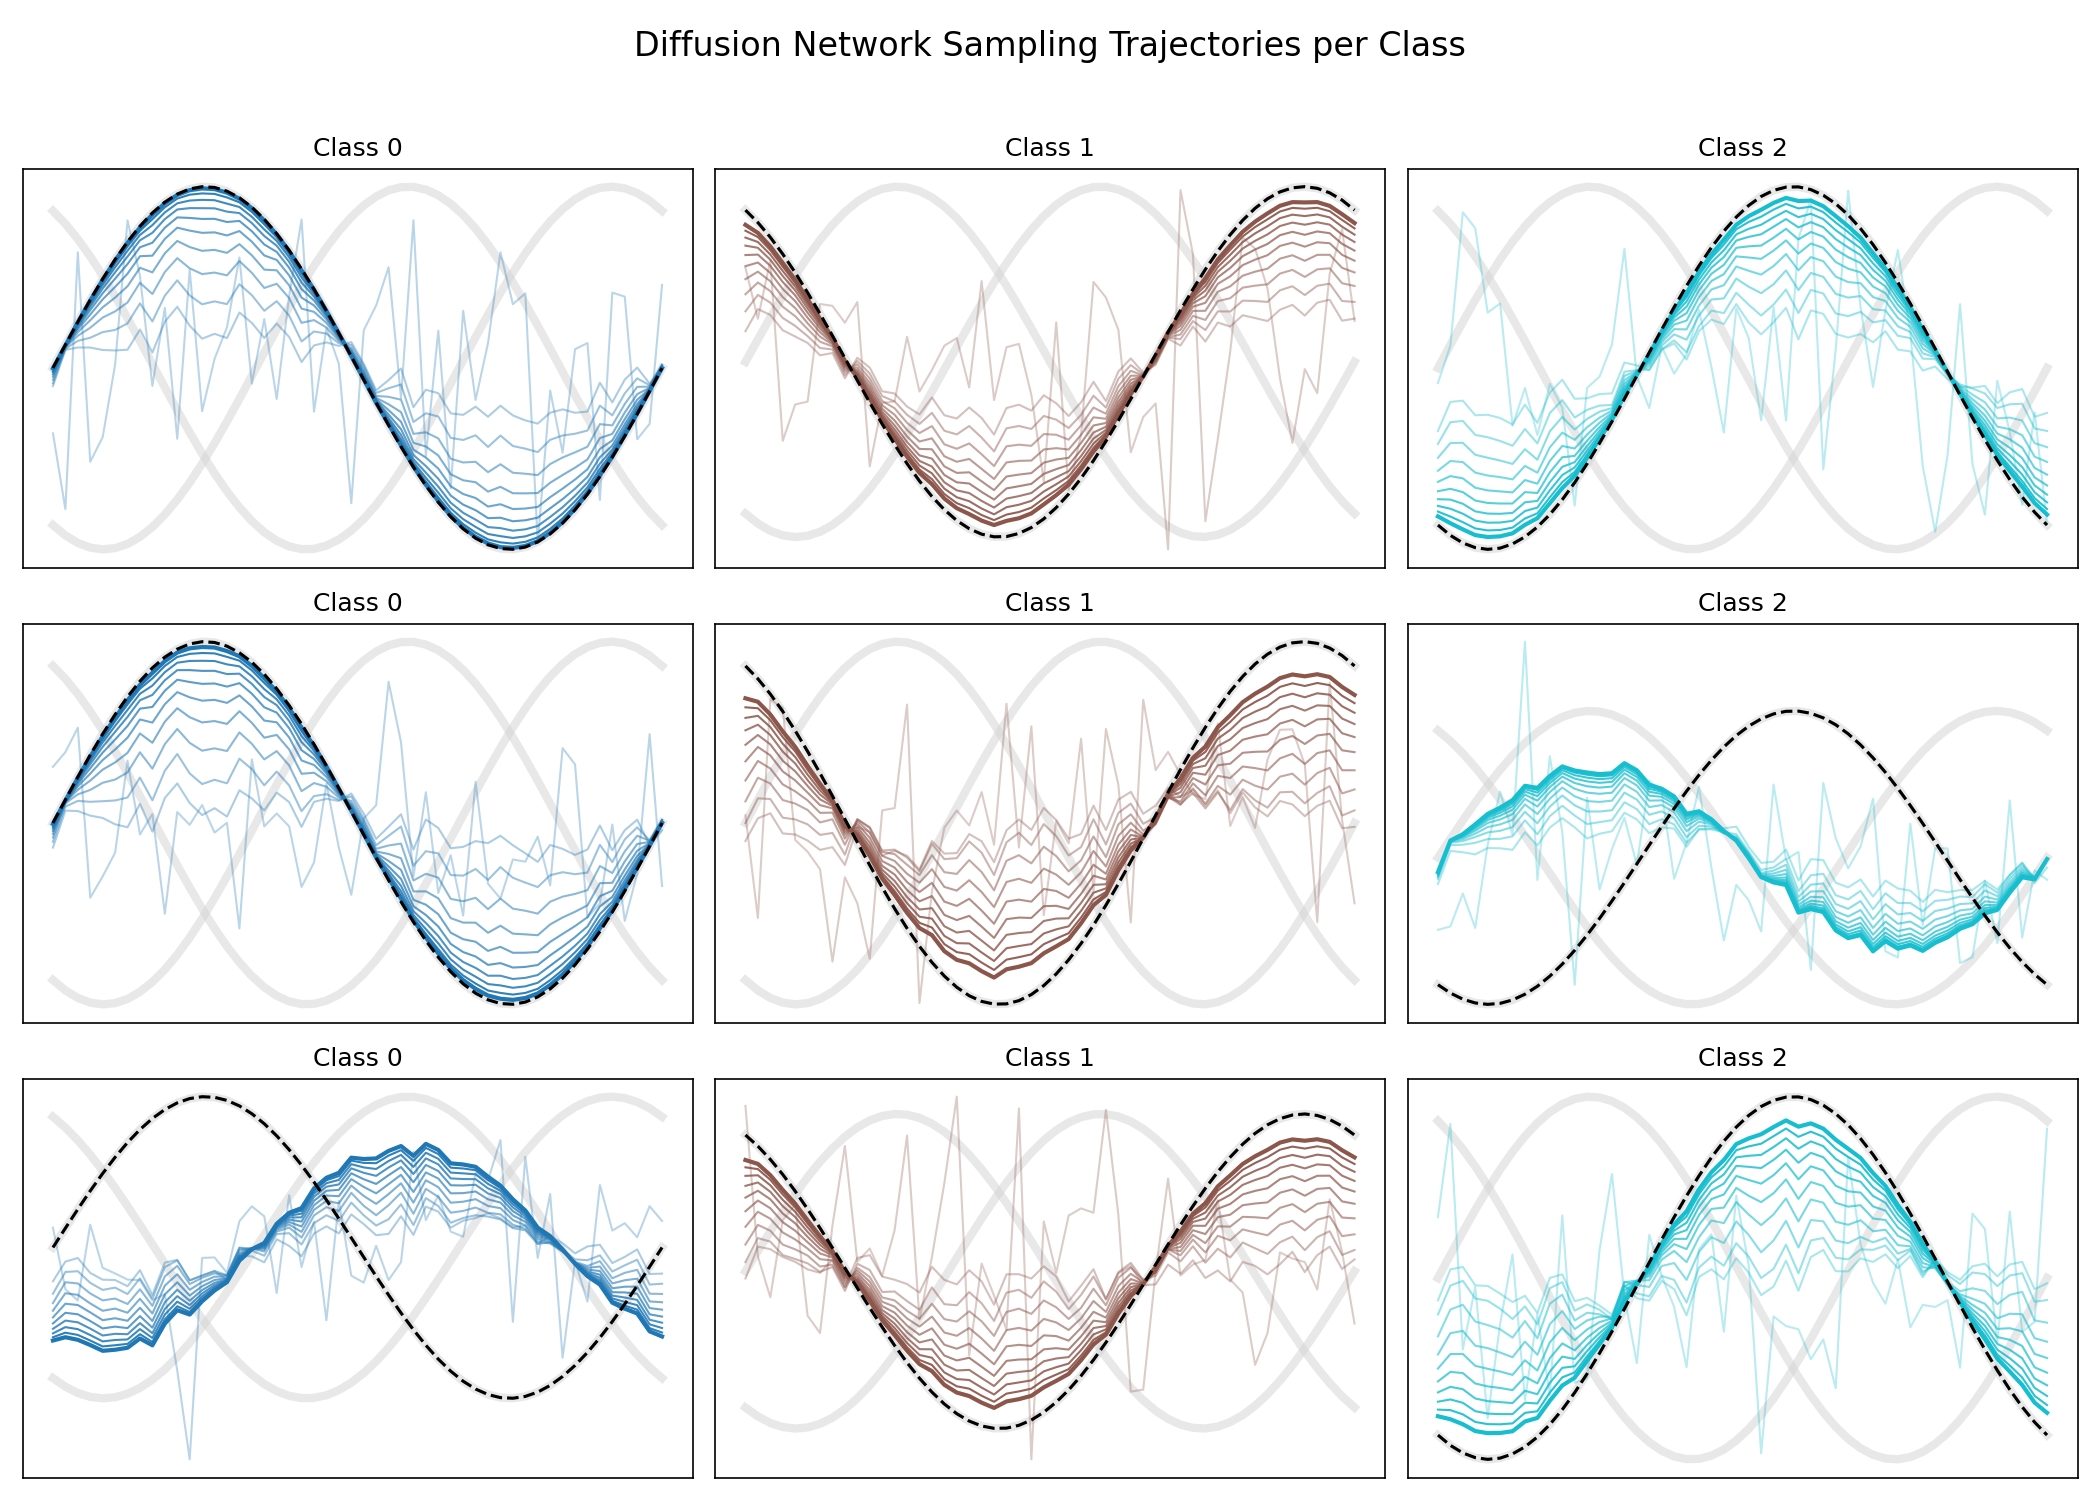
\includegraphics[width=\textwidth]{images/diffusion_network_sampling.png}
\caption{Denoising trajectories for 9 generated signals. Each panel shows 10 intermediate steps from noise to final output. The gray curve is the class target.}
\label{fig:step-by-step}
\end{figure}

%------------------------------------------------------------------------------
\subsubsection*{Summary and Perspective}

This example illustrates the core idea of diffusion-based generation: from noise to signal, guided by side information. While we use class labels here, the conditioning input could be general — spatial context, metadata, or even a short natural language prompt.

In weather and climate modeling, this approach can be extended to:
\begin{itemize}
    \item Generate ensemble forecast members from coarse NWP input,
    \item Downscale global simulations to local weather fields,
    \item Impute missing or corrupted observations,
    \item Build hybrid models integrating physics and data.
\end{itemize}

We now have a powerful framework to model structured distributions over functions — not by directly learning the output, but by learning how to refine noise into data.

%------------------------------------------------------------------------------
%
%------------------------------------------------------------------------------
\subsection{Why it Works: Diffusion Network Theory for the Scalar Case}

To better understand the probabilistic nature of diffusion models, we consider a one-dimensional (scalar) example. Let the original data distribution be a Gaussian:
\[
x_0 \sim \mathcal{N}(\mu_0, \sigma_0^2),
\]
with a concrete choice of parameters \( \mu_0 = 3 \), \( \sigma_0^2 = 1 \). The forward diffusion step adds Gaussian noise:
\[
x_1 = x_0 + \epsilon, \quad \epsilon \sim \mathcal{N}(0, \sigma^2).
\]
By basic facts on Gaussian distributions, the distribution of \( x_1 \) becomes:
\[
x_1 \sim \mathcal{N}(\mu_0, \sigma_0^2 + \sigma^2).
\]

%------------------------------------------------------------------------------
\paragraph{Optimal Denoiser.}
The optimal denoiser in the mean-squared error sense is the conditional expectation:
\[
f^*(x_1) := \mathbb{E}[x_0 \mid x_1].
\]
Lets do the little derivation here. Assume \( x_0 \sim \mathcal{N}(\mu_0, \sigma_0^2) \) is the clean signal, and the observed noisy signal is \( x_1 = x_0 + \epsilon \), where \( \epsilon \sim \mathcal{N}(0, \sigma^2) \) is independent Gaussian noise. Then, using Bayes' theorem, the posterior distribution of \( x_0 \) given \( x_1 \) is:
\[
p(x_0 \mid x_1) = \frac{p(x_1 \mid x_0) \cdot p(x_0)}{p(x_1)}.
\]
Let us recall a standard identity for univariate Gaussian distributions, noting that $p(x_1)$ serves as normalization constant in the Bayes formula. The (unnormalized) product of two Gaussians 
\[
\mathcal{N}(x \mid \mu_1, \sigma_1^2) \cdot \mathcal{N}(x \mid \mu_2, \sigma_2^2) 
\propto \mathcal{N}\left(x \mid \mu_{\times}, \sigma_{\times}^2\right),
\]
is again a Gaussian with:
\begin{align*}
\sigma_{\times}^2 &= \left( \frac{1}{\sigma_1^2} + \frac{1}{\sigma_2^2} \right)^{-1}
= \frac{\sigma_1^2 \sigma_2^2}{\sigma_1^2 + \sigma_2^2}, \\
\mu_{\times} &= \sigma_{\times}^2 \left( \frac{\mu_1}{\sigma_1^2} + \frac{\mu_2}{\sigma_2^2} \right)
= \frac{\sigma_2^2 \mu_1 + \sigma_1^2 \mu_2}{\sigma_1^2 + \sigma_2^2}.
\end{align*}
We now apply this directly to the posterior:
\[
p(x_0 \mid x_1) \propto p(x_1 \mid x_0) \cdot p(x_0),
\]
with:
\[
p(x_0) = \mathcal{N}(x_0 \mid \mu_0, \sigma_0^2), \qquad
p(x_1 \mid x_0) = \mathcal{N}(x_1 \mid x_0, \sigma^2),
\]
which we can rewrite as:
\[
p(x_1 \mid x_0) = \mathcal{N}(x_0 \mid x_1, \sigma^2),
\]
so the product becomes:
\[
p(x_0 \mid x_1) \propto \mathcal{N}(x_0 \mid \mu_0, \sigma_0^2) \cdot \mathcal{N}(x_0 \mid x_1, \sigma^2).
\]
By the above rule, the posterior is again Gaussian:
\[
p(x_0 \mid x_1) = \mathcal{N}(x_0 \mid \mu_{\text{post}}, \sigma_{\text{post}}^2),
\]
with:
\begin{align*}
\sigma_{\text{post}}^2 &= \frac{\sigma_0^2 \cdot \sigma^2}{\sigma_0^2 + \sigma^2}, \\
\mu_{\text{post}} &= \frac{\sigma^2 \mu_0 + \sigma_0^2 x_1}{\sigma_0^2 + \sigma^2}.
\end{align*}
This means
\begin{equation}
f^*(x_1) = \mathbb{E}[x_0 \mid x_1] = \mu_{\text{post}} = \frac{\sigma^2 \mu_0 + \sigma_0^2 x_1}{\sigma_0^2 + \sigma^2}
= x_1 + (\mu_0 - x_1 )\cdot \frac{\sigma^2}{\sigma_0^2 + \sigma^2}.
\label{opt estimator}
\end{equation}
Hence, the optimal denoiser is a linear function pulling \( x_1 \) toward \( \mu_0 \), and reducing the variance.  
Using 
\[
\mathrm{Var}(aX+b) = a^2 \cdot Var(X)
\]
the variance of \( f^*(x_1) \) in dependence of $x_1$ is calculated by:
\[
\mathrm{Var}(f^*(x_1)) = \left( \frac{\sigma_0^2}{\sigma_0^2 + \sigma^2} \right)^2 \cdot \mathrm{Var}(x_1) = \frac{\sigma_0^4}{\sigma_0^2 + \sigma^2}.
\]
To recover the original distribution, we must sample from the full posterior:
\[
x_0 = f^*(x_1) + \sqrt{\sigma_{\text{post}}^2} \cdot \xi, \quad \xi \sim \mathcal{N}(0, 1).
\]
Then, the total variance becomes:
\[
\mathrm{Var}(x_0) = \mathrm{Var}(f^*(x_1)) + \sigma_{\text{post}}^2
= \frac{\sigma_0^4 + \sigma_0^2 \cdot \sigma^2}{\sigma_0^2 + \sigma^2}
= \frac{\sigma_0^2 (\sigma_0^2 + \sigma^2)}{\sigma_0^2 + \sigma^2}
= \sigma_0^2.
\]

%------------------------------------------------------------------------------
\paragraph{Why Iterative Sampling is Necessary.}
A single denoising step, modeled as the conditional expectation \( f^*(x_1) = \mathbb{E}[x_0 \mid x_1] \), does not recover the original mean \( \mu_0 \) of the data distribution. Instead, it produces a posterior mean \( \mu_{\text{post}} \) that is a weighted combination of \( x_1 \) and \( \mu_0 \). The output is therefore still biased by the noise in \( x_1 \).

To progressively move towards the original distribution \( \mathcal{N}(\mu_0, \sigma_0^2) \), multiple denoising steps are needed. Each step slightly reduces the noise and shifts the estimate closer to the clean data manifold. This is the essence of iterative sampling in diffusion models: a sequence of reverse transitions from noise to data.

Suppose we add Gaussian noise in \( n \) steps, where each step adds noise with standard deviation \( \sigma / n \). The variance of the noise added in step \( k \) is thus \( \sigma_k^2 = \sigma^2 / n^2 \), and the total noise variance after all \( n \) steps is:
\[
\sigma_{\text{total}}^2 = \sum_{k=1}^n \frac{\sigma^2}{n^2} = \frac{\sigma^2}{n}.
\]
Let \( x_n \) denote the final noisy sample. To denoise step-by-step, we apply the optimal estimator in reverse order, using the posterior mean:
\[
\mathbb{E}[x_{k-1} \mid x_k] = (1 - \gamma_k) x_k + \gamma_k \mu^{(prior)}_{k-1},
\]
where
\[
\gamma_k
= \frac{\frac{\sigma^2}{n^2}}{\sigma_0^2 + \frac{(k-1)\sigma^2}{n^2} + \frac{\sigma^2}{n^2}}
= \frac{\sigma^2}{{n^2 \sigma_0^2} + k \sigma^2}.
\]
and \( \mu^{(prior)}_{k-1} \) is the expected prior mean of \( x_{k-1} \) before seeing $x_k$, obtained from previous steps, such as $\mu_0$ if we did not rescale our original signal or the rescaled values when rescaling is used. This defines a recursion:
\[
x_{k-1} = (1 - \gamma_k) x_k + \gamma_k \mu_0 = x_k + \gamma_k ( \mu_0 - x_k),
\]
starting from \( x_n \). Since $\gamma_k$ is consistently larger than 
\[
\gamma_{min} := \frac{\sigma^2}{n^2 \sigma_0^2 + n \sigma^2}, 
\] 
unrolling this recursion 
\[
x_{k-1} = (1 - \gamma_{\min}) x_k + \gamma_{\min} \mu_0
\]
for \( k = n, n-1, \dotsc, 1 \), with fixed \( \gamma_{\min} \in (0, 1) \), we obtain (based the standard geometric series argument)
\[
x_0 = (1 - \gamma_{\min})^n x_n + \left(1 - (1 - \gamma_{\min})^n \right) \mu_0
\rightarrow \mu_0, \;\; n \rightarrow \infty, 
\]
i.e.\ it shows that the denoising path progressively pulls the expectation back toward the original mean $\mu_0$. Thus, iterative denoising converges to the true mean in the limit of infinitely many small noise-injection and denoising steps.

This confirms that iterative denoising with many small steps recovers the original distribution mean — even though each individual step is only a small correction.

%------------------------------------------------------------------------------
\paragraph{Conclusion.} This simple scalar example demonstrates a crucial aspect of diffusion models:
\begin{itemize}
    \item The optimal denoiser \( f^*(x_k) \) estimates the \emph{mean} of the reverse distribution.
    \item To match the original data distribution, one must \emph{sample} from the full posterior, which includes adding back calibrated noise.
    \item This justifies the stochastic reverse process used in diffusion models, where noise is injected in each denoising step.
\end{itemize}

%==============================================================================
% 
%==============================================================================
\section{Flexible Graph Networks for Learning from Sparse Observations}

\subsection{A Naive Approach: Learning Functions from Sparse Observations}

In this first implementation, we train a Graph Neural Network (GNN) to reconstruct simple functions (sine and cosine) from partial observations on a one-dimensional grid. The setup is intentionally minimal and includes all components required to construct, train, and apply a graph-based model. Later sections will analyze and generalize this setup.

\paragraph{Overview:}
We aim to learn a mapping from sparse observations to a full function profile by training on synthetically generated sine and cosine functions with random phases. Observations are available at every $M$-th grid point. The GNN uses a fixed neighborhood structure defined by $K$-nearest neighbors.

\vspace{1em}
\noindent The complete workflow includes the following components:

\begin{itemize}
  \item Creating the spatial grid.
  \item Defining the graph connectivity.
  \item Designing the GNN architecture.
  \item Training the model on sampled functions.
  \item Testing the model on larger and more complex domains.
\end{itemize}

\begin{figure}[ht]
  \centering
  \begin{tabular}{ccc}
    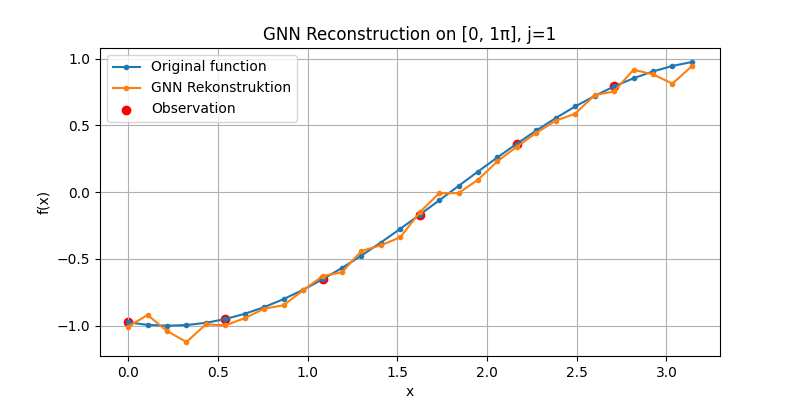
\includegraphics[width=0.3\textwidth]{images/gnn_obs_naive_j1_jj1_0.png} &
    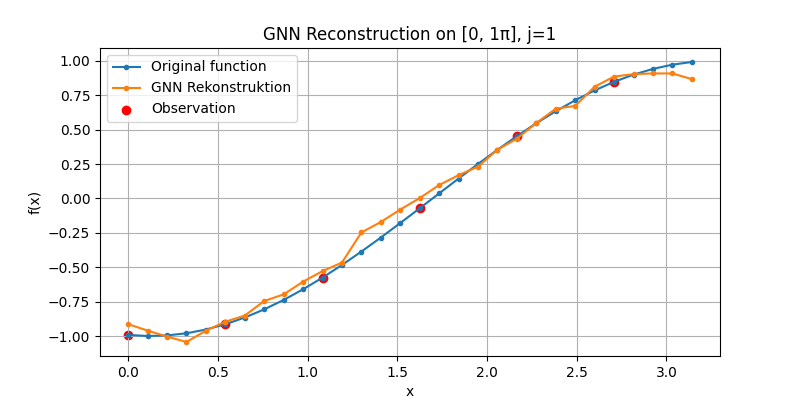
\includegraphics[width=0.3\textwidth]{images/gnn_obs_naive_j1_jj1_1.png} &
    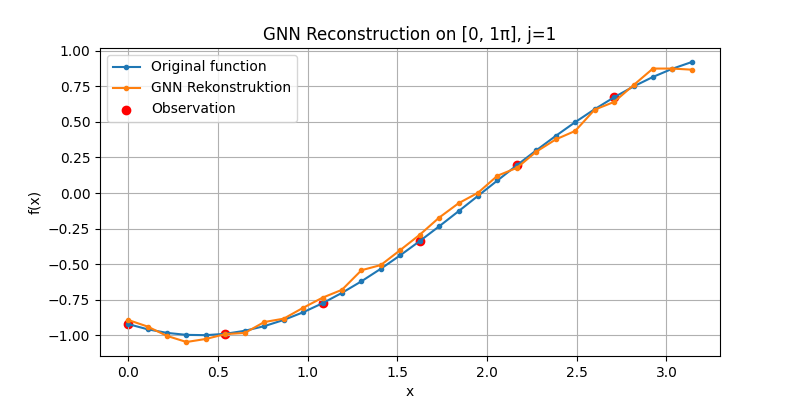
\includegraphics[width=0.3\textwidth]{images/gnn_obs_naive_j1_jj1_2.png} \\
    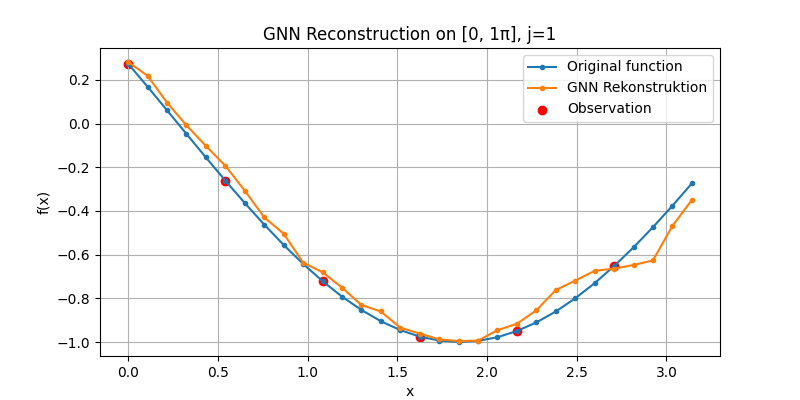
\includegraphics[width=0.3\textwidth]{images/gnn_obs_naive_j1_jj1_3.png} &
    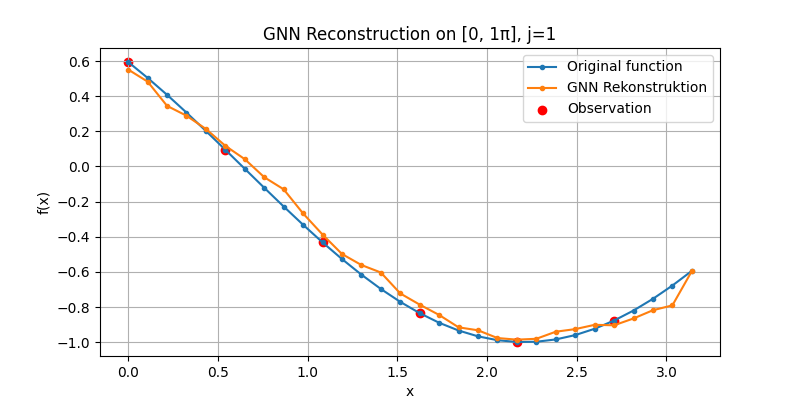
\includegraphics[width=0.3\textwidth]{images/gnn_obs_naive_j1_jj1_4.png} &
    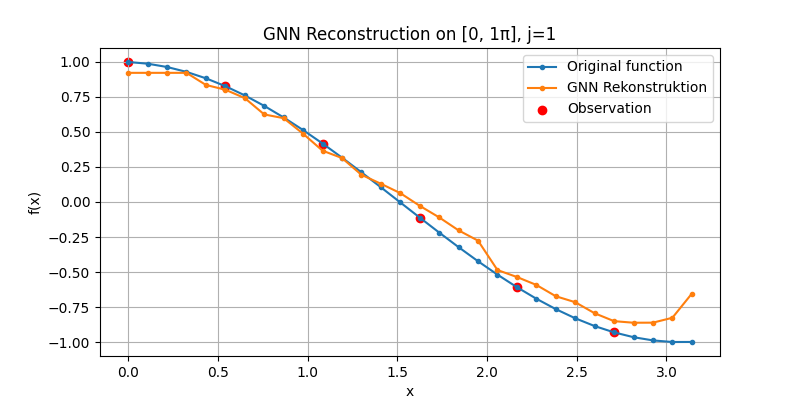
\includegraphics[width=0.3\textwidth]{images/gnn_obs_naive_j1_jj1_5.png} \\
    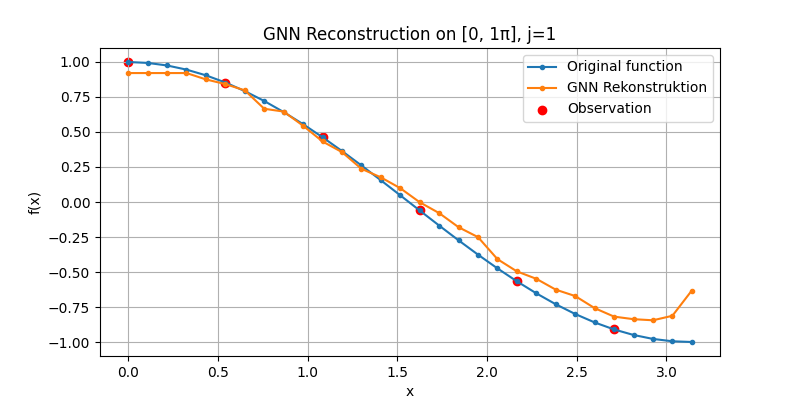
\includegraphics[width=0.3\textwidth]{images/gnn_obs_naive_j1_jj1_6.png} &
    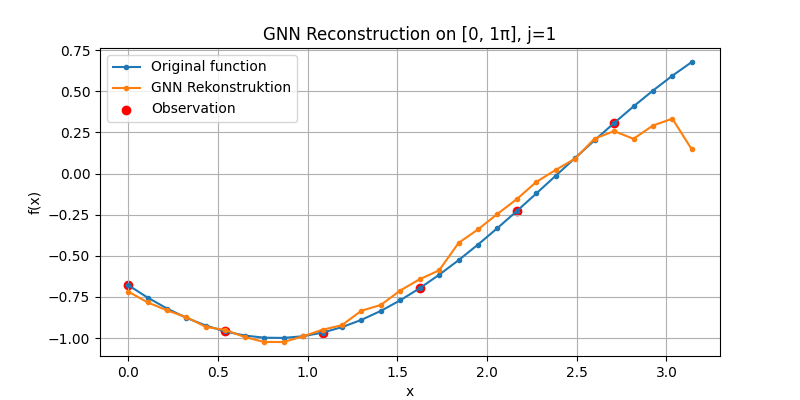
\includegraphics[width=0.3\textwidth]{images/gnn_obs_naive_j1_jj1_7.png} &
    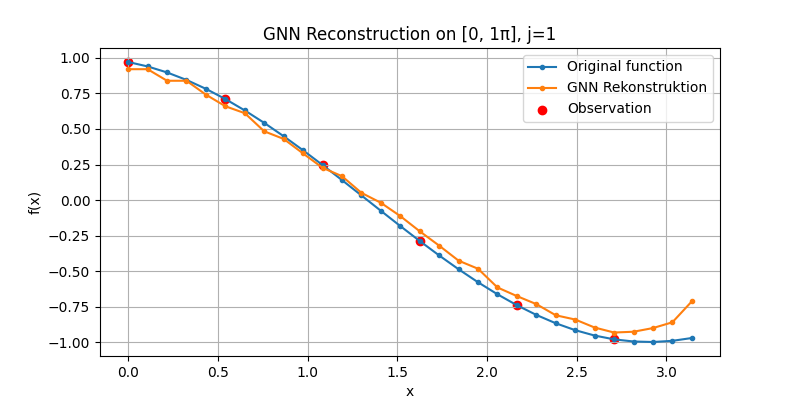
\includegraphics[width=0.3\textwidth]{images/gnn_obs_naive_j1_jj1_8.png} \\
  \end{tabular}
  \caption{GNN reconstructions for $f(x) = \cos(x + \phi)$ on $[0, \pi]$ with different phases. Each panel shows the original function, sparse observations, and the GNN prediction.}
  \label{fig:gnn_j1_jj1}
\end{figure}


\paragraph{Step 1: Libraries and Parameter Setup}

\begin{codeonly}{Imports and Parameters}
import torch
import torch.nn as nn
import torch.nn.functional as F
import numpy as np
import matplotlib.pyplot as plt

N = 30           # Number of grid points
M = 5            # Every M-th point is observed
K = 3            # Number of neighbors per node
num_epochs = 201
num_samples = 200
lr = 0.01

x_grid = torch.linspace(0, np.pi, N)
\end{codeonly}

\paragraph{Step 2: Graph Construction}

Each node is connected to itself and its $K$ neighbors on both sides. This creates a fixed undirected graph.

\begin{codeonly}{Graph Construction}
edges = []
for i in range(N):
    edges.append((i, i))  # Self-loop
    for k in range(1, K + 1):
        if i - k >= 0:
            edges.append((i, i - k))
        if i + k < N:
            edges.append((i, i + k))
edge_index = torch.tensor(edges).T  # [2, num_edges]
\end{codeonly}

\paragraph{Step 3: Model Architecture}

We define a basic GNN architecture with two message-passing layers. Each layer aggregates features from neighboring nodes and applies a linear transformation.

\begin{codeonly}{Model Definition}
class GNNLayer(nn.Module):
    def __init__(self, dim):
        super().__init__()
        self.self_lin = nn.Linear(dim, dim)
        self.neigh_lin = nn.Linear(dim, dim)

    def forward(self, x, edge_index):
        row, col = edge_index
        agg = torch.zeros_like(x)
        agg.index_add_(0, row, x[col])
        return F.relu(self.self_lin(x) + self.neigh_lin(agg))

class GNN(nn.Module):
    def __init__(self, in_dim=3, hidden=64):
        super().__init__()
        self.input_proj = nn.Linear(in_dim, hidden)
        self.gnn1 = GNNLayer(hidden)
        self.gnn2 = GNNLayer(hidden)
        self.out = nn.Linear(hidden, 1)

    def forward(self, x, edge_index):
        x = F.relu(self.input_proj(x))
        x = self.gnn1(x, edge_index)
        x = self.gnn2(x, edge_index)
        return self.out(x).squeeze(-1)

model = GNN(in_dim=3)
opt = torch.optim.Adam(model.parameters(), lr=lr)
\end{codeonly}

\begin{figure}[ht]
  \centering
  \begin{tabular}{cccc}
    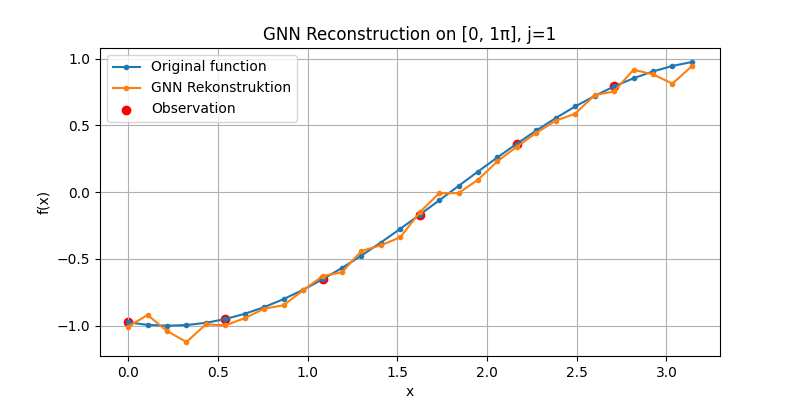
\includegraphics[width=0.23\textwidth]{images/gnn_obs_naive_j1_jj1_0.png} &
    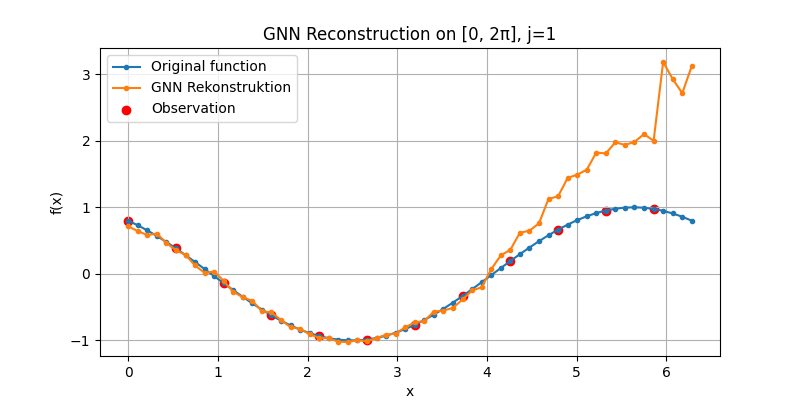
\includegraphics[width=0.23\textwidth]{images/gnn_obs_naive_j1_jj2_0.png} &
    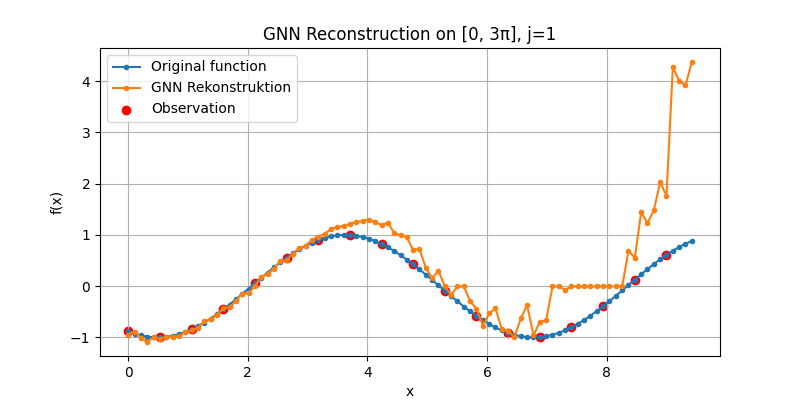
\includegraphics[width=0.23\textwidth]{images/gnn_obs_naive_j1_jj3_0.png} &
    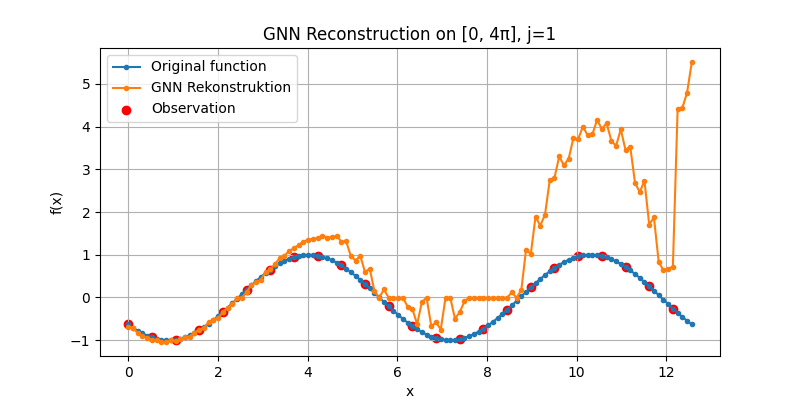
\includegraphics[width=0.23\textwidth]{images/gnn_obs_naive_j1_jj4_0.png} \\
    $\texttt{j=1, jj=1}$ & $\texttt{j=1, jj=2}$ & $\texttt{j=1, jj=3}$ & $\texttt{j=1, jj=4}$ \\
  \end{tabular}
  \caption{Generalization of the GNN to longer intervals. All test functions use $f(x) = \cos(x + \phi)$ but are evaluated on increasing domains $[0, jj \cdot \pi]$ with $jj = 1, 2, 3, 4$. The model was trained only on $[0, \pi]$.}
  \label{fig:gnn_generalization_jj}
\end{figure}


\paragraph{Step 4: Training Loop}

The model is trained to reconstruct either a sine or cosine function with random phase. Observations are only available at every $M$-th grid point. The input to each node includes the position $x$, the (masked) observation value, and a binary mask.

\begin{codeonly}{Training Loop}
for epoch in range(num_epochs):
    losses = []
    for _ in range(num_samples):
        phase = torch.rand(1).item() * np.pi
        f_type = torch.randint(0, 2, (1,)).item()
        f = lambda x: torch.sin(x + phase) if f_type == 0 else torch.cos(x + phase)
        y_true = f(x_grid)

        mask = torch.zeros(N)
        mask[::M] = 1.0
        obs_y = y_true * mask

        x_feat = torch.stack([x_grid, obs_y, mask], dim=1)

        model.train()
        pred = model(x_feat, edge_index)
        loss = F.mse_loss(pred, y_true)
        opt.zero_grad()
        loss.backward()
        opt.step()
        losses.append(loss.item())

    if epoch % 50 == 0:
        print(f"Epoch {epoch}: Loss = {np.mean(losses):.6f}")
\end{codeonly}

\begin{figure}[ht]
  \centering
  \begin{tabular}{cccc}
    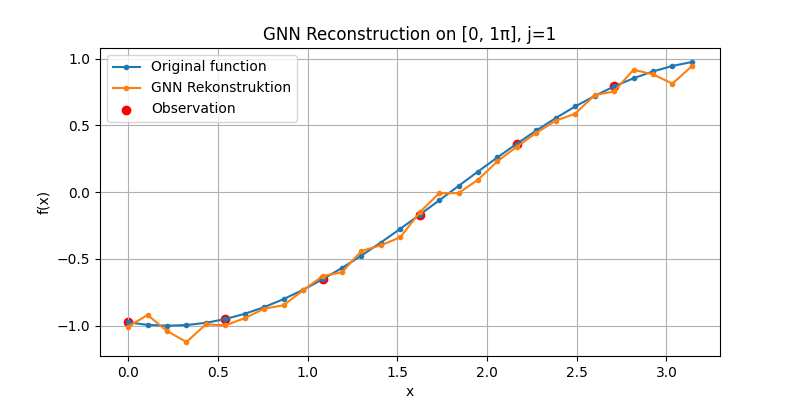
\includegraphics[width=0.23\textwidth]{images/gnn_obs_naive_j1_jj1_0.png} &
    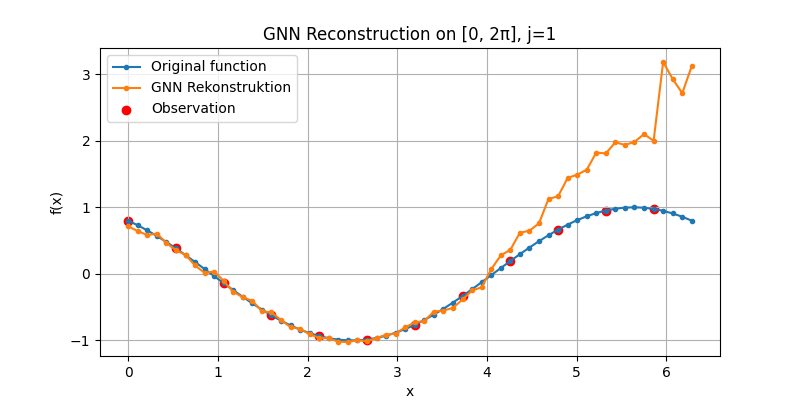
\includegraphics[width=0.23\textwidth]{images/gnn_obs_naive_j1_jj2_0.png} &
    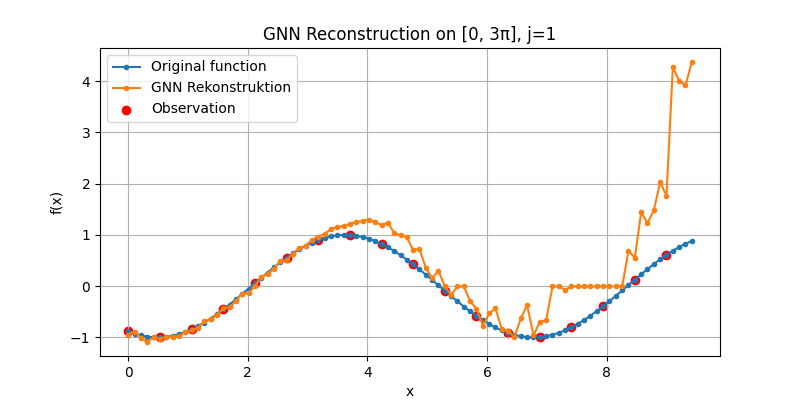
\includegraphics[width=0.23\textwidth]{images/gnn_obs_naive_j1_jj3_0.png} &
    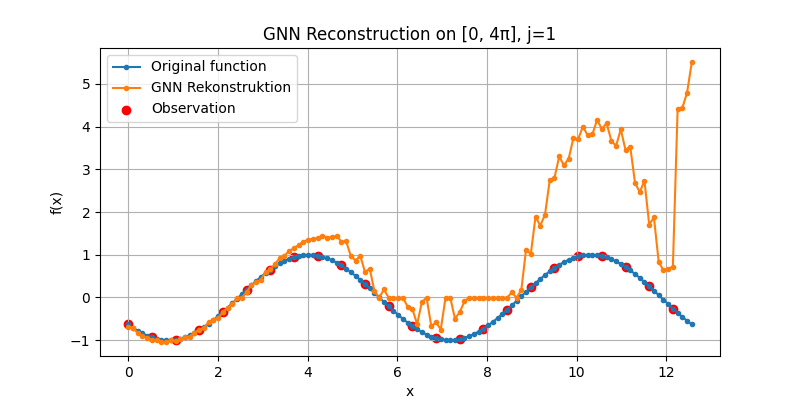
\includegraphics[width=0.23\textwidth]{images/gnn_obs_naive_j1_jj4_0.png} \\
    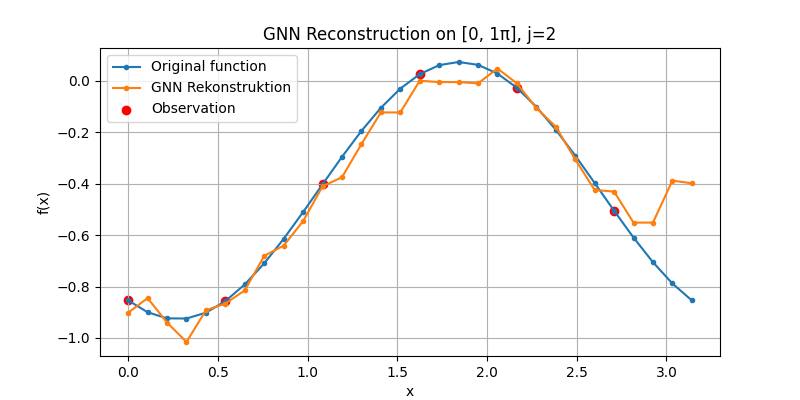
\includegraphics[width=0.23\textwidth]{images/gnn_obs_naive_j2_jj1_0.png} &
    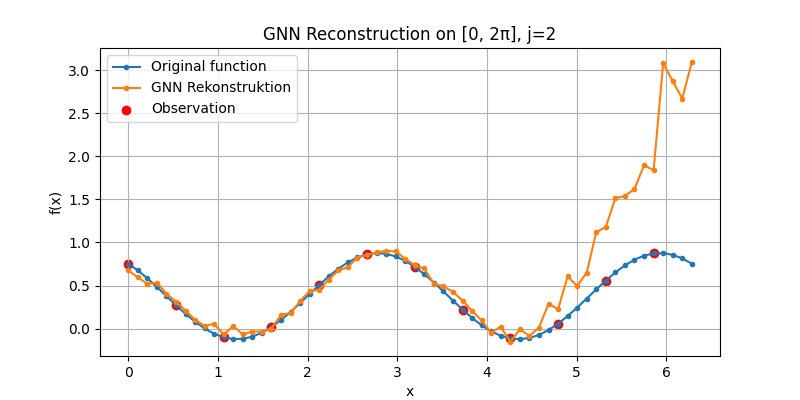
\includegraphics[width=0.23\textwidth]{images/gnn_obs_naive_j2_jj2_0.png} &
    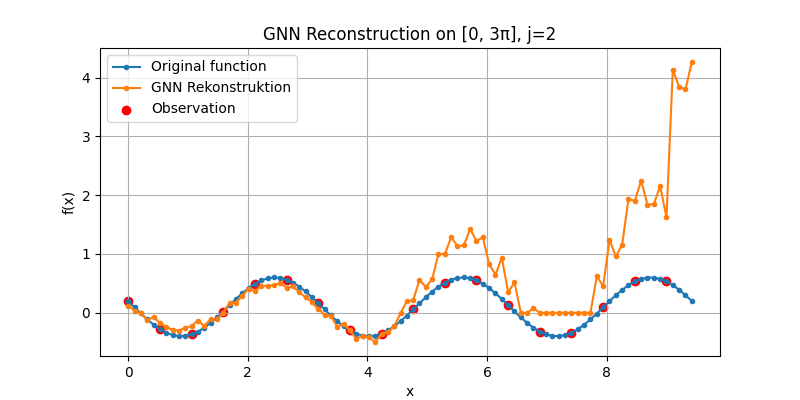
\includegraphics[width=0.23\textwidth]{images/gnn_obs_naive_j2_jj3_0.png} &
    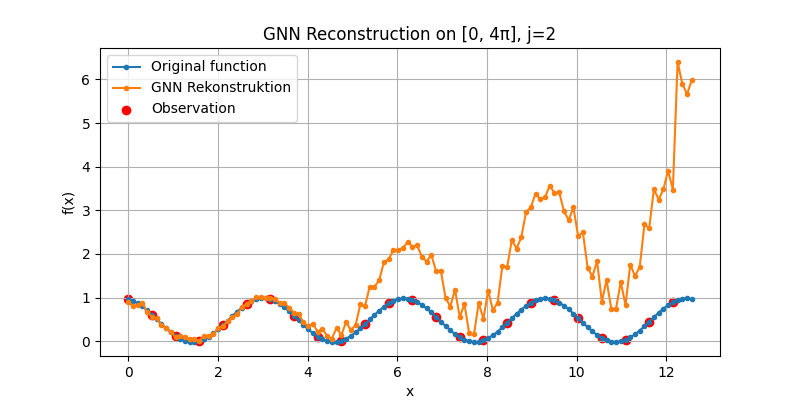
\includegraphics[width=0.23\textwidth]{images/gnn_obs_naive_j2_jj4_0.png} \\
    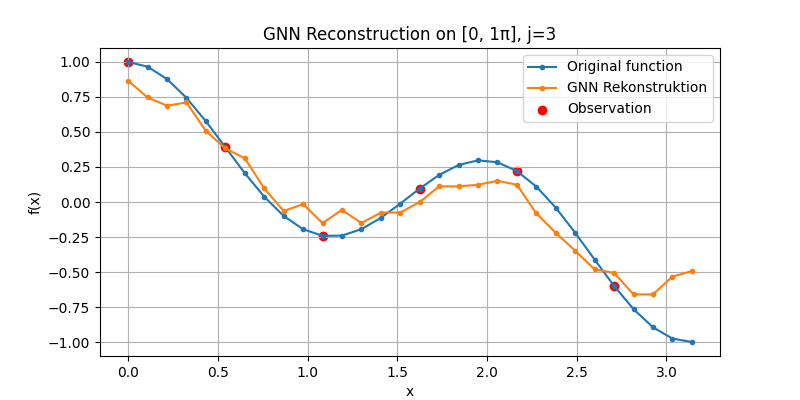
\includegraphics[width=0.23\textwidth]{images/gnn_obs_naive_j3_jj1_0.png} &
    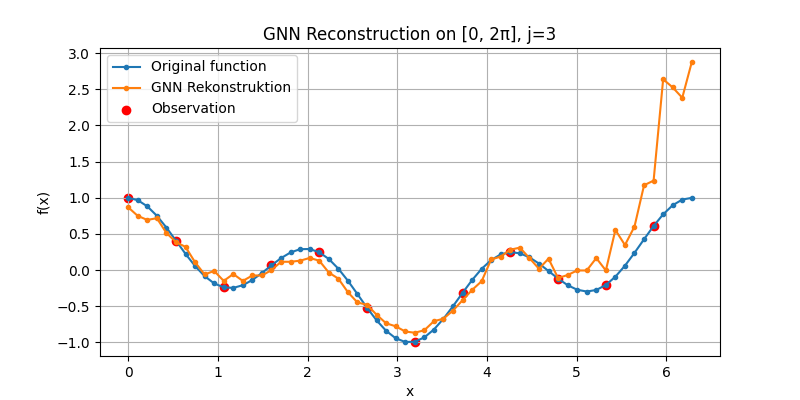
\includegraphics[width=0.23\textwidth]{images/gnn_obs_naive_j3_jj2_0.png} &
    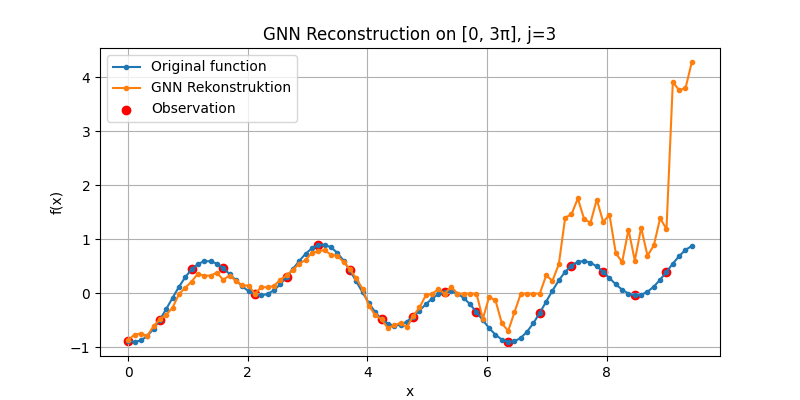
\includegraphics[width=0.23\textwidth]{images/gnn_obs_naive_j3_jj3_0.png} &
    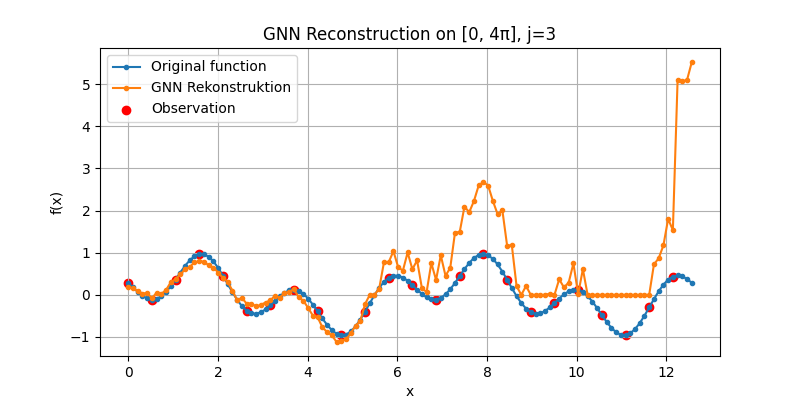
\includegraphics[width=0.23\textwidth]{images/gnn_obs_naive_j3_jj4_0.png} \\
    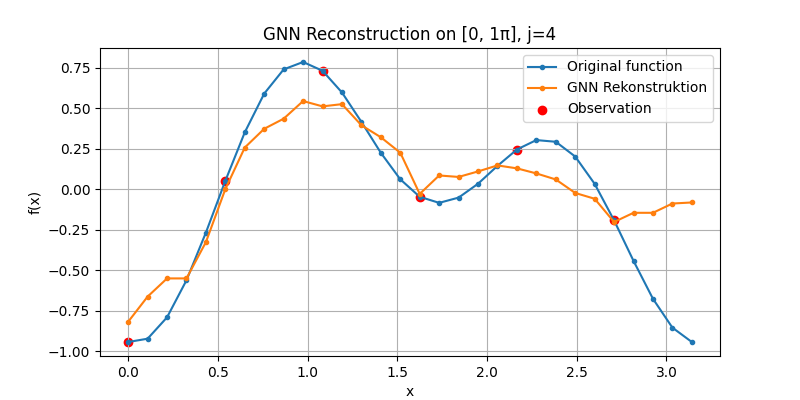
\includegraphics[width=0.23\textwidth]{images/gnn_obs_naive_j4_jj1_0.png} &
    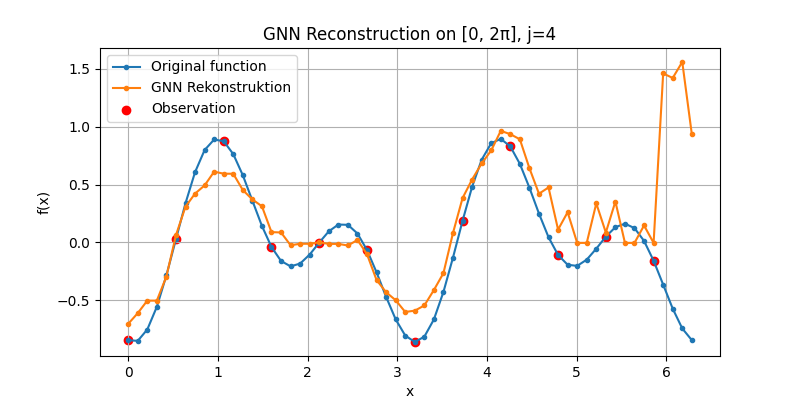
\includegraphics[width=0.23\textwidth]{images/gnn_obs_naive_j4_jj2_0.png} &
    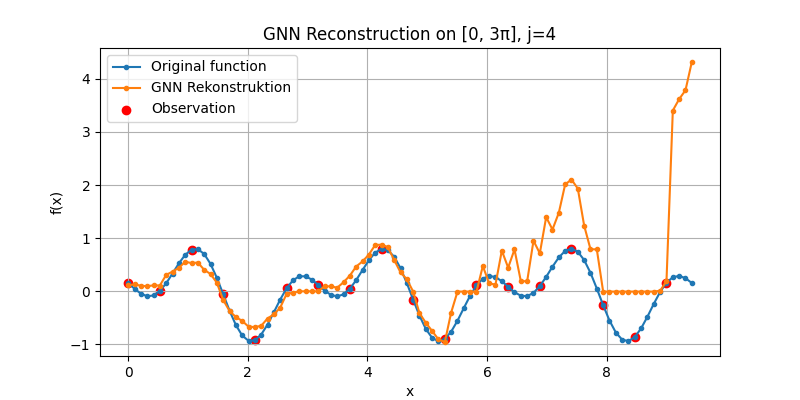
\includegraphics[width=0.23\textwidth]{images/gnn_obs_naive_j4_jj3_0.png} &
    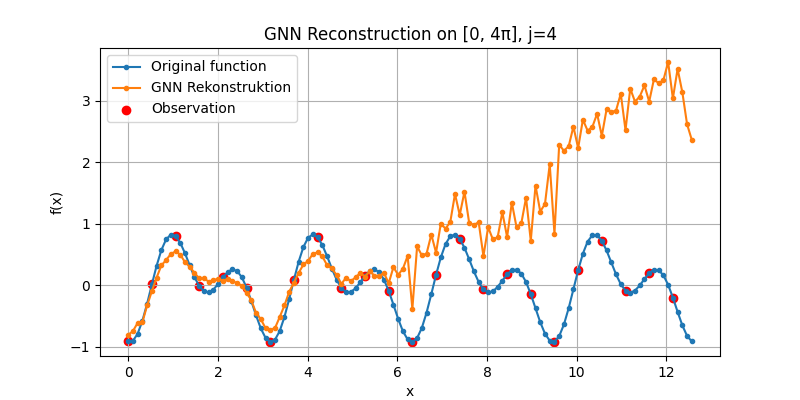
\includegraphics[width=0.23\textwidth]{images/gnn_obs_naive_j4_jj4_0.png} \\
  \end{tabular}
  \caption{GNN reconstruction results for functions $f(x) = \cos(x + \phi)\cos((j-1)x)$ with increasing frequency ($j = 1$ to $4$) and interval length ($jj = 1$ to $4$). Each image shows prediction based on sparse observations.}
  \label{fig:gnn_jj_generalization_full}
\end{figure}


\paragraph{Step 5: Testing on Extended Domains}

We evaluate the trained model on functions of the form $f(x) = \cos(x + \phi)\cos((j-1)x)$ over extended intervals $[0, j \cdot \pi]$. This tests the generalization ability of the GNN.

\begin{codeonly}{Test Function and Evaluation}
def run_test(j, jj):
    N_test = jj * 30
    x_test_grid = torch.linspace(0, jj * np.pi, N_test)

    phi_test = torch.rand(1).item() * np.pi
    f_test = lambda x: torch.cos(x + phi_test) * torch.cos((j - 1) * x)
    y_test = f_test(x_test_grid)

    mask = torch.zeros(N_test)
    mask[::M] = 1.0
    obs = y_test * mask
    x_feat_test = torch.stack([x_test_grid, obs, mask], dim=1)

    edges = []
    for i in range(N_test):
        edges.append((i, i))  # Self-loop
        for k in range(1, K + 1):
            if i - k >= 0:
                edges.append((i, i - k))
            if i + k < N_test:
                edges.append((i, i + k))
    edge_index_test = torch.tensor(edges).T

    model.eval()
    with torch.no_grad():
        pred_test = model(x_feat_test, edge_index_test)

    plt.figure(figsize=(8, 4))
    plt.plot(x_test_grid, y_test, '.-', label="Original function")
    plt.plot(x_test_grid, pred_test, '.-', label="GNN Rekonstruktion")
    plt.scatter(x_test_grid[::M], y_test[::M], color='red', label="Observation")
    plt.title(f"GNN Reconstruction on [0, {jj}pi], j={j}")
    plt.xlabel("x")
    plt.ylabel("f(x)")
    plt.grid(True)
    plt.legend()
    plt.show()

for j in range(1, 5):
    run_test(1, jj=j)
    run_test(j, jj=j)
\end{codeonly}

\paragraph{Conclusion}

This naive setup already demonstrates the capacity of GNNs to reconstruct continuous functions from sparse data. In the next sections, we will explore how to generalize this setup and test whether absolute positional information (i.e., $x$) is truly necessary for accurate reconstructions.

%==============================================================================
%
%==============================================================================
\subsection{Coordinate-Free GNN: Learning from Observations Alone}

In this variation, we explore the idea of removing the coordinate $x$ from the GNN input entirely. Instead of feeding the spatial location explicitly into the model, we rely solely on two pieces of information per node:
\begin{itemize}
  \item the observed function value (or zero if unobserved),
  \item a binary mask indicating whether the value was observed.
\end{itemize}
The graph topology itself continues to encode spatial relationships via $K$-nearest neighbors. This setup allows the network to learn purely from **relational** and **structural** information.

\vspace{0.5em}
\noindent
To implement this, we change the input feature dimension to 2 and remove $x$ from the input vector:

\begin{codeonly}{Model Without Coordinates}
class GNN(nn.Module):
    def __init__(self, in_dim=2, hidden=64):
        ...
x_feat = torch.stack([obs_y, mask], dim=1)  # No x-coordinate
model2 = GNN(in_dim=2)
\end{codeonly}

\vspace{0.5em}
\noindent
The training loop remains identical. For testing, we run the same function `run\_test(j, jj, tag)` but again exclude the coordinate $x$ from the input:

\begin{codeonly}{Coordinate-Free Testing}
x_feat_test = torch.stack([obs, mask], dim=1)
pred_test = model2(x_feat_test, edge_index_test)
plt.savefig(f"gnn_obs_no_pos_j{j}_jj{jj}_{tag}.png")
\end{codeonly}


\begin{figure}[ht]
  \centering
  \begin{tabular}{cccc}
    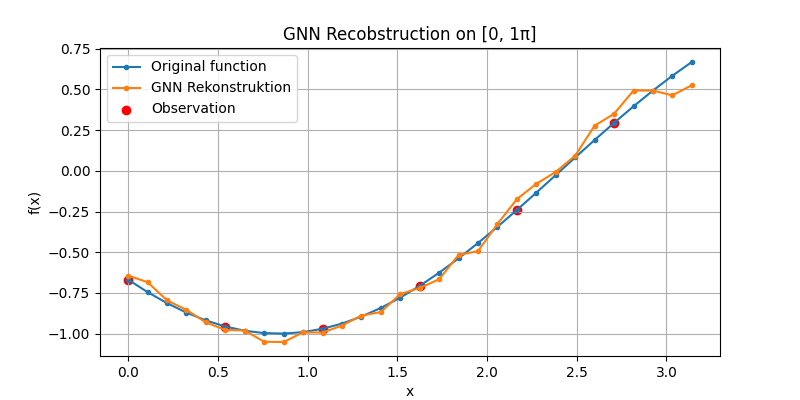
\includegraphics[width=0.23\textwidth]{images/gnn_obs_no_pos_j1_jj1_0.png} &
    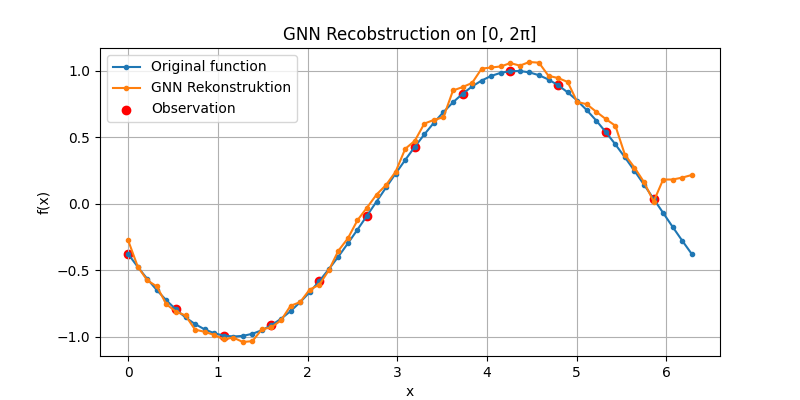
\includegraphics[width=0.23\textwidth]{images/gnn_obs_no_pos_j1_jj2_0.png} &
    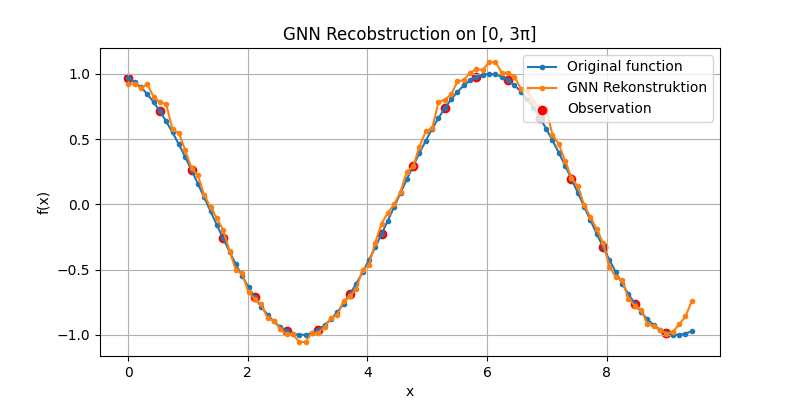
\includegraphics[width=0.23\textwidth]{images/gnn_obs_no_pos_j1_jj3_0.png} &
    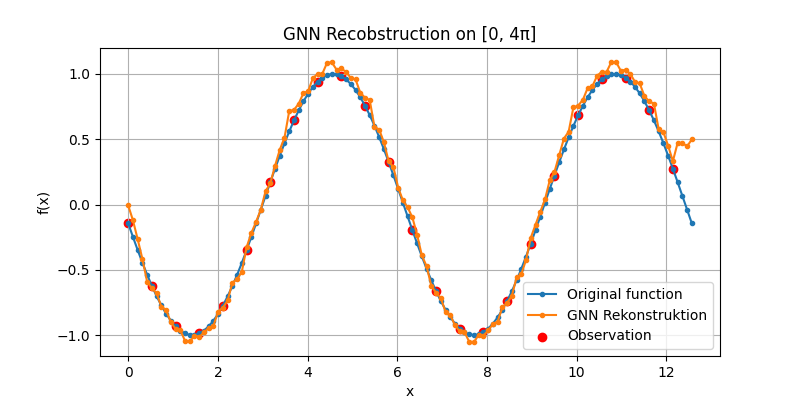
\includegraphics[width=0.23\textwidth]{images/gnn_obs_no_pos_j1_jj4_0.png} \\
    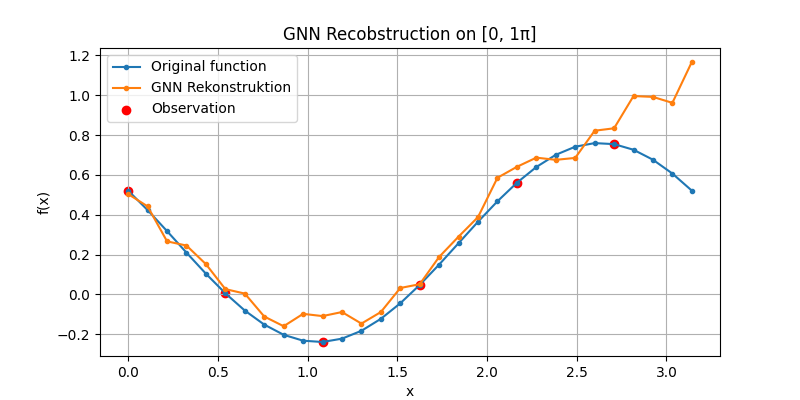
\includegraphics[width=0.23\textwidth]{images/gnn_obs_no_pos_j2_jj1_0.png} &
    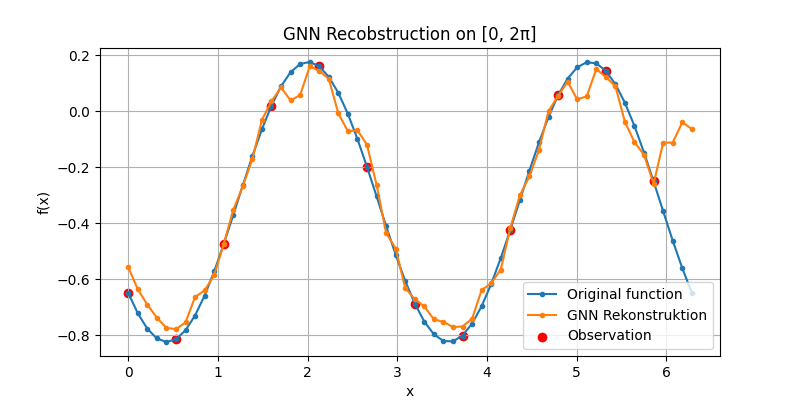
\includegraphics[width=0.23\textwidth]{images/gnn_obs_no_pos_j2_jj2_0.png} &
    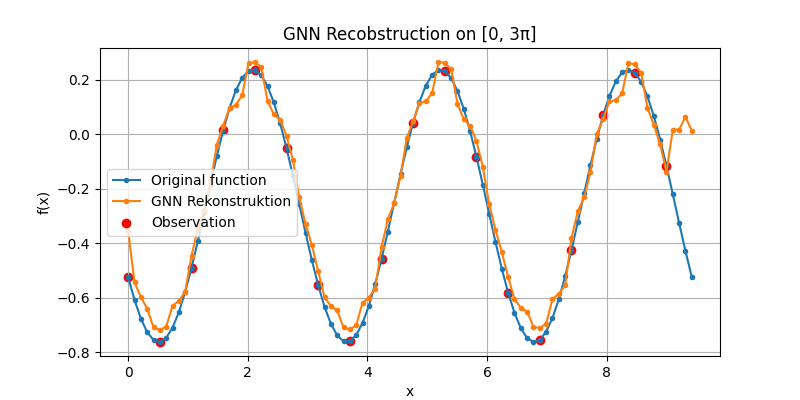
\includegraphics[width=0.23\textwidth]{images/gnn_obs_no_pos_j2_jj3_0.png} &
    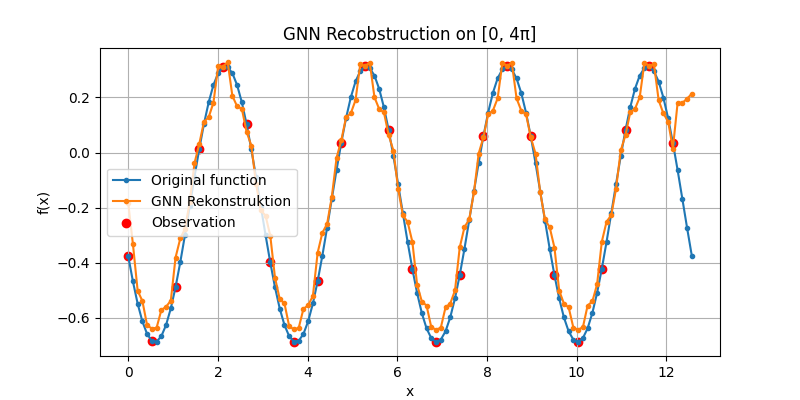
\includegraphics[width=0.23\textwidth]{images/gnn_obs_no_pos_j2_jj4_0.png} \\
    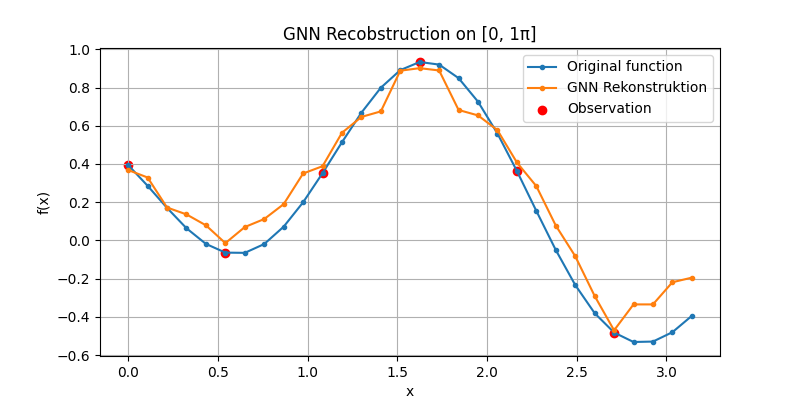
\includegraphics[width=0.23\textwidth]{images/gnn_obs_no_pos_j3_jj1_0.png} &
    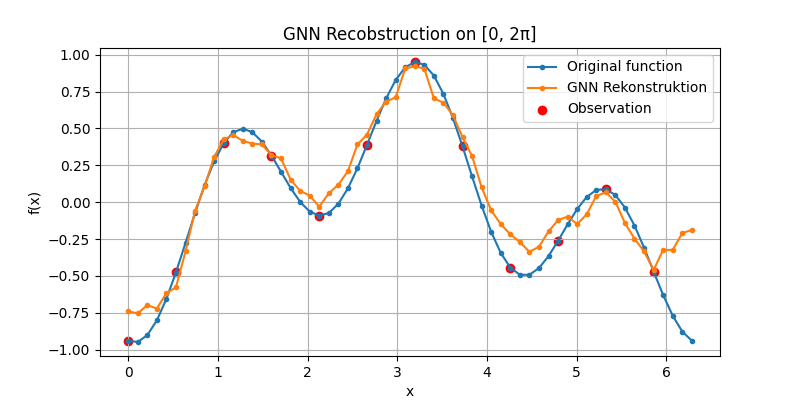
\includegraphics[width=0.23\textwidth]{images/gnn_obs_no_pos_j3_jj2_0.png} &
    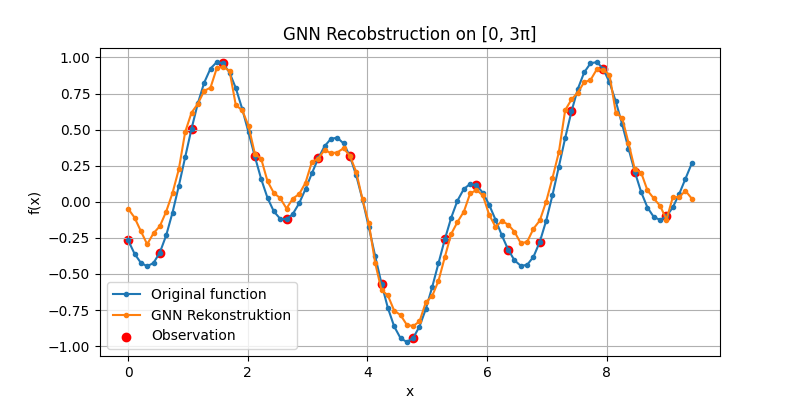
\includegraphics[width=0.23\textwidth]{images/gnn_obs_no_pos_j3_jj3_0.png} &
    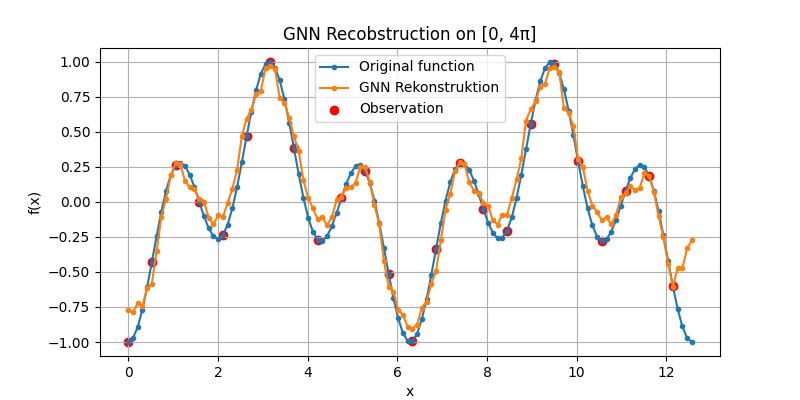
\includegraphics[width=0.23\textwidth]{images/gnn_obs_no_pos_j3_jj4_0.png} \\
    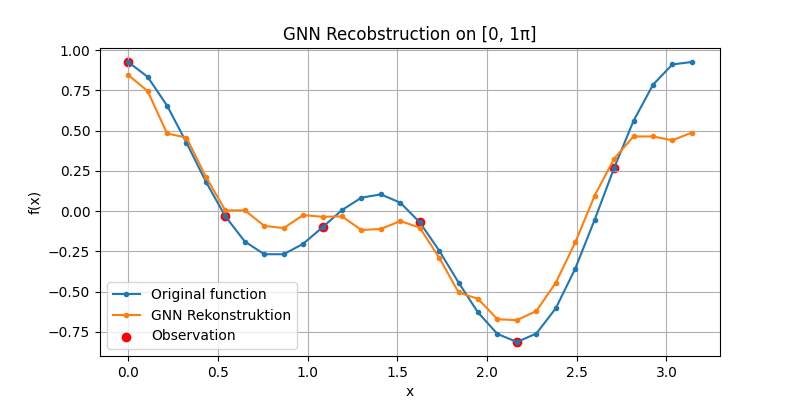
\includegraphics[width=0.23\textwidth]{images/gnn_obs_no_pos_j4_jj1_0.png} &
    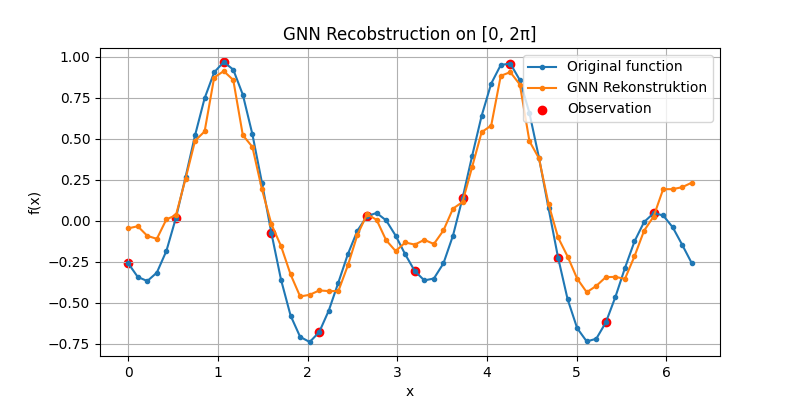
\includegraphics[width=0.23\textwidth]{images/gnn_obs_no_pos_j4_jj2_0.png} &
    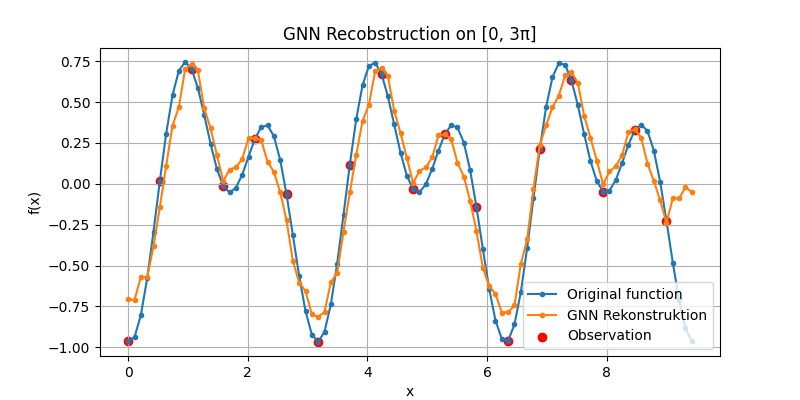
\includegraphics[width=0.23\textwidth]{images/gnn_obs_no_pos_j4_jj3_0.png} &
    \includegraphics[width=0.23\textwidth]{images/gnn_obs_no_pos_j4_jj4_0.png} \\
  \end{tabular}
  \caption{GNN reconstructions without coordinate input. Each panel shows $f(x) = \cos(x + \phi)\cos((j-1)x)$ reconstructed from sparse observations, across increasing frequency $j = 1\ldots4$ and domain size $jj = 1\ldots4$. The model was trained without using $x$-position as input and on shifted sines only, no higher modes in the training dataset.}
  \label{fig:gnn_no_pos_grid}
\end{figure}

\paragraph{Surprising Result: Better Generalization Without Coordinates}

This variant performs {\em significantly better} when generalizing to longer domains and higher-frequency functions. While this may appear counterintuitive at first, the reason is rooted in how the model interprets the coordinate input.

When $x$ is included as a feature, the GNN must learn to "undo" the fact that $x$ changes range across intervals. For example, $x \in [0,\pi]$ during training but later $x \in [0,4\pi]$ during testing — unless the network has learned that $x$ is irrelevant, it may overfit to this scale and fail to generalize.

By removing $x$, we force the network to focus on {\bf local patterns} and {\bf relational geometry} encoded in the graph structure — which remains scale-invariant and consistent across test domains.

%==============================================================================
%
%==============================================================================
\section{Exploring Graph Structures in Detail}

\subsection{Inspecting the Number of Trainable Parameters}

Graph neural networks (GNNs) operate on graph-structured data by aggregating and transforming node features according to a given graph topology. The structure of the graph is provided through the {\tt edge\_index}, which specifies the connections between nodes, while the trainable parameters of the model are applied uniformly across the entire graph.

\begin{codeonly}{Edge Index and GNN Forward Pass}
# x: [N, F] feature matrix for N nodes, each with F features
# edge_index: [2, E] matrix with E directed edges (source, target)

x = model(x, edge_index)
\end{codeonly}

The {\tt edge\_index} is a $2 \times E$ tensor that defines the spatial structure of the graph by listing all $E$ edges as source-target pairs. It governs how information flows between nodes, but it does not introduce any additional trainable parameters. Instead, the weights in a GNN are shared across all nodes and edges, making the model invariant to the graph size and applicable to different domains.

Each layer in the model—such as linear projections and message-passing operations—has its own set of parameters, which are learned during training. These parameters determine {\bf how} node features are updated, while the {\tt edge\_index} determines {\bf where} messages are exchanged. As a result, we can reuse the same trained model architecture and weights on graphs of varying size or structure, as long as the input feature format remains consistent.

{\bf Parameter Numbers.} We now explore the exact number of trainable parameters in our models using a simple Python function and interpret how input dimensionality affects model complexity.

To measure the size of a model, we compute the total number of trainable parameters using the function {\tt nelement()} for each parameter tensor. The command shown sums over all layers and returns a single integer that quantifies the model's capacity.

\begin{codeonly}{One Linear Model Parameters}
sum([param.nelement() for param in model.parameters()])
\end{codeonly}

To inspect the complexity of our models, we define a simple Python function that iterates over all trainable parameters and prints their names, shapes, and counts:

\begin{codeonly}{Simple Parameter Summary}
def simple_param_summary(model):
    print('-'*80)
    total = 0
    print("Layer Summary:")
    for name, param in model.named_parameters():
        count = param.numel()
        total += count
        print(f"{name:30} | shape: {list(param.shape)} | params: {count}")
    print(f"\nTotal trainable parameters: {total}")
\end{codeonly}

This function produces an informative overview, showing the parameter count for each layer and the overall model. We apply it to two model variants: {\bf model}, which uses the full feature vector \texttt{[x, val, mask]} with input dimension 3, and {\bf model2}, which omits the coordinate and uses only \texttt{[val, mask]} with input dimension 2.

\vspace{1em}
{\bf Result for model (with coordinate):}

\begin{verbatim}
input_proj.weight              | shape: [64, 3] | params: 192
input_proj.bias                | shape: [64]    | params: 64
gnn1.self_lin.weight           | shape: [64, 64] | params: 4096
gnn1.self_lin.bias             | shape: [64]     | params: 64
gnn1.neigh_lin.weight          | shape: [64, 64] | params: 4096
gnn1.neigh_lin.bias            | shape: [64]     | params: 64
gnn2.self_lin.weight           | shape: [64, 64] | params: 4096
gnn2.self_lin.bias             | shape: [64]     | params: 64
gnn2.neigh_lin.weight          | shape: [64, 64] | params: 4096
gnn2.neigh_lin.bias            | shape: [64]     | params: 64
out.weight                     | shape: [1, 64]  | params: 64
out.bias                       | shape: [1]      | params: 1
Total trainable parameters: 16961
\end{verbatim}

\vspace{1em}
{\bf Result for model2 (without coordinate):}

\begin{verbatim}
input_proj.weight              | shape: [64, 2] | params: 128
input_proj.bias                | shape: [64]    | params: 64
... (identical hidden layers and output)
Total trainable parameters: 16897
\end{verbatim}

The only difference lies in the first linear layer. With three input features, the input projection layer has $64 \times 3 + 64 = 256$ parameters, while with two inputs it has $64 \times 2 + 64 = 192$ parameters. This difference of exactly 64 parameters matches the total discrepancy between the models.

\vspace{1em}
{\bf Interpretation:} The rest of the model—two GNN layers with shared hidden size and the final output projection—remains identical in both cases. This small change in input dimensionality helps us isolate the effect of using or omitting positional information ($x$) while keeping model capacity nearly the same.

This method is a convenient way to audit model size, debug unexpected parameter growth, or document the impact of architectural choices.

%==============================================================================
%
%==============================================================================
\subsection{Marching through the Graph Processing}

\begin{figure}[ht]
    \centering
    \includegraphics[width=\textwidth]{images/graph_structure.pdf}
    \caption{Schematic of the GNN architecture with input projection, two GNN layers using neighborhood aggregation, and output transformation.}
    \label{fig:gnn-structure}
\end{figure}

%------------------------------------------------------------------------------
%
%------------------------------------------------------------------------------
{\bf Step 1: Raw Node Input Features.} Each node $i$ in the graph carries basic local information encoded as a 2-dimensional vector:
\[
\mathbf{x}_i^{(0)} =
\begin{bmatrix}
\mathrm{val}_i \\
\mathrm{mask}_i
\end{bmatrix} \in \mathbb{R}^2.
\]

This input consists of:
\begin{itemize}
  \item $\mathrm{val}_i$: the observed function value at the node $i$, or $0$ if the value is unobserved,
  \item $\mathrm{mask}_i \in \{0, 1\}$: a binary indicator specifying whether the value is present ($1$) or missing ($0$).
\end{itemize}

The full input feature matrix for all $N$ nodes in the graph is:
\[
X^{(0)} =
\begin{bmatrix}
--- & \mathbf{x}_1^{(0)} & --- \\
--- & \mathbf{x}_2^{(0)} & --- \\
& \vdots & \\
--- & \mathbf{x}_N^{(0)} & ---
\end{bmatrix}
\in \mathbb{R}^{N \times 2}.
\]

\medskip
{\bf Motivation:} This minimal feature representation provides the model with:
\begin{itemize}
  \item The available measurement data (only at selected nodes),
  \item An explicit signal of which nodes are observed and which are not,
  \item A compact and domain-agnostic encoding that avoids absolute positional information.
\end{itemize}

\medskip
These raw inputs are passed to the first learnable layer of the network — the linear projection — which maps them into a higher-dimensional latent space for further processing and message passing.


%------------------------------------------------------------------------------
%
%------------------------------------------------------------------------------
{\bf Step 2: Linear Input Projection Layer.} Each node in the graph is initially represented by a 2-dimensional feature vector:
\[
\mathbf{x}_i^{(0)} = 
\begin{bmatrix}
\mathrm{val}_i \\
\mathrm{mask}_i
\end{bmatrix}
\in \mathbb{R}^2,
\]
where
\begin{itemize}
  \item $\mathrm{val}_i$ is the observed function value at node $i$ (or zero if unobserved),
  \item $\mathrm{mask}_i \in \{0, 1\}$ indicates whether the observation is present.
\end{itemize}

These raw features are passed through a learned linear transformation to project them into a higher-dimensional feature space:
\[
\mathbf{x}_i^{(1)} = \sigma\left( W \mathbf{x}_i^{(0)} + \mathbf{b} \right), \quad W \in \mathbb{R}^{64 \times 2}, \quad \mathbf{b} \in \mathbb{R}^{64},
\]
where $\sigma$ is the ReLU activation function applied component-wise:
\[
\sigma(z) = \max(0, z).
\]

This operation is applied independently to all $N$ nodes in the graph, resulting in a projected feature matrix
\[
X^{(1)} \in \mathbb{R}^{N \times 64}.
\]

\medskip
{\bf Purpose:} This step enables the model to:
\begin{itemize}
  \item Interpret the semantic meaning of the raw inputs,
  \item Learn different representations for observed and unobserved nodes,
  \item Embed all nodes into a common latent space for message passing.
\end{itemize}

\medskip
{\bf Interpretation:} The weights in $W$ determine how much influence the observed value and the mask have on each of the 64 embedding dimensions. For example:
\begin{itemize}
  \item Some dimensions may be dominated by the presence or absence of data,
  \item Others may capture approximate magnitudes or trends across the domain.
\end{itemize}

This projected representation is then passed to the GNN layers, where it is refined through interaction with neighboring nodes.

%------------------------------------------------------------------------------
%
%------------------------------------------------------------------------------
{\bf Step 3: Message Passing with GNNLayer.} After the input features have been projected to the latent space $\mathbb{R}^{64}$, the node embeddings are updated using the graph structure. This happens through two successive {\tt GNNLayer} blocks, each of which applies message passing followed by a learned transformation.

For the first layer, the input is $X^{(1)} \in \mathbb{R}^{N \times 64}$. The message passing operation updates each node $i$ based on its own features and the features of its neighbors, as defined by the edge list {\tt edge\_index}.

\medskip
Each {\tt GNNLayer} performs the following update:
\[
\mathbf{x}_i^{(\ell+1)} = \sigma\left(
W_{\text{self}} \mathbf{x}_i^{(\ell)} +
W_{\text{neigh}} \sum_{j \in \mathcal{N}(i)} \mathbf{x}_j^{(\ell)}
\right),
\]
where:
\begin{itemize}
  \item $\mathbf{x}_i^{(\ell)} \in \mathbb{R}^{64}$ is the node feature vector at layer $\ell$,
  \item $\mathcal{N}(i)$ is the set of neighbors of node $i$ (including self-loop),
  \item $W_{\text{self}}, W_{\text{neigh}} \in \mathbb{R}^{64 \times 64}$ are learned weight matrices,
  \item $\sigma$ is the ReLU activation function.
\end{itemize}

The neighborhood aggregation is computed via:
\[
\mathbf{a}_i = \sum_{j \in \mathcal{N}(i)} \mathbf{x}_j^{(\ell)},
\]
which is then linearly transformed and added to the transformed self-information. In PyTorch, this is implemented by accumulating neighbor features with the operation:
\begin{verbatim}
agg = torch.zeros_like(x)
agg.index_add_(0, row, x[col])
\end{verbatim}
where {\tt edge\_index = [row, col]} encodes all directed edges from node {\tt col[k]} to node {\tt row[k]}.

\medskip
{\bf Interpretation:} This layer learns how to combine a node's own state with information from its local neighborhood. It does so in a trainable, nonlinear way, which enables it to reconstruct smooth or structured functions based on sparsely observed values.

Two such GNN layers are applied in sequence in the model, each refining the representation based on a wider receptive field (i.e., information from nodes up to two hops away).

%------------------------------------------------------------------------------
%
%------------------------------------------------------------------------------
{\bf Step 4: Output Projection.} After two rounds of message passing, each node $i$ is represented by a refined hidden state vector:
\[
\mathbf{x}_i^{(3)} \in \mathbb{R}^{64}.
\]

To convert this latent representation into a scalar prediction (e.g., an estimate of the underlying function value at node $i$), the model applies a final linear projection:
\[
\hat{y}_i = w^\top \mathbf{x}_i^{(3)} + b,
\quad w \in \mathbb{R}^{64}, \quad b \in \mathbb{R}.
\]

This is implemented in PyTorch as:
\begin{verbatim}
self.out = nn.Linear(64, 1)
\end{verbatim}

Applied to all $N$ nodes, the output becomes:
\[
\hat{y} =
\begin{bmatrix}
\hat{y}_1 \\
\hat{y}_2 \\
\vdots \\
\hat{y}_N
\end{bmatrix}
\in \mathbb{R}^{N},
\]
which is compared to the true function $y \in \mathbb{R}^{N}$ during training using a mean squared error loss:
\[
\mathcal{L} = \frac{1}{N} \sum_{i=1}^N (\hat{y}_i - y_i)^2.
\]

\medskip
{\bf Purpose:} This step transforms the latent node embedding back into the physical space of scalar function values. It completes the reconstruction process by producing a prediction for every node in the graph — observed or not.

\medskip
{\bf Interpretation:} The model learns to extract the relevant features through the graph structure and to compress them into a meaningful final scalar output. Since the same output transformation is applied to every node, the model remains fully permutation-invariant with respect to the node order.

\medskip
{\bf Final Remarks on Structure and Complexity.}
The graph network architecture described in this section is compact yet expressive. It processes node-wise inputs in four clearly structured stages as shown in Figure \ref{fig:gnn-structure}: 
\begin{itemize}
\item
input feature encoding, 
\item
projection into a latent space, 
\item
two rounds of message passing, and 
\item
a final output projection. 
\end{itemize}
Each {\tt GNNLayer} updates node representations by combining a self-weighted embedding with a shared transformation of its neighbors — using just two weight matrices per layer, independent of the graph's size or shape. 

The total number of parameters remains modest (16{,}961 in the case of three input features), with the majority concentrated in the two GNN layers. Despite this simplicity, the model captures complex interactions across the graph and generalizes naturally to different domains. Crucially, the graph structure itself is not learned but provided externally via {\tt edge\_index}, making the model both interpretable and highly adaptable. This layered design, along with consistent weight sharing and localized aggregation, gives the network its power to generalize, interpolate, and reconstruct global behavior from sparse, local input.


%==============================================================================
%
%==============================================================================
\section{PyTorch Lightning and PyTorch Geometric}

Modern PyTorch workflows benefit greatly from using helper libraries that simplify model training and extend PyTorch with domain-specific components. Two such libraries are:

\begin{itemize}
  \item {\bf PyTorch Lightning:} A high-level wrapper around PyTorch that structures training, logging, and hardware management into a clean and scalable format.
  \item {\bf PyTorch Geometric (PyG):} A specialized library for graph neural networks (GNNs), enabling message passing, pooling, and graph data structures.
\end{itemize}

These libraries integrate seamlessly and can be used together to train graph-based models in a clean and efficient way.

To follow the examples in this tutorial, the following packages must be installed. Installation should be done in a Python 3.9+ environment with PyTorch already installed.

\begin{codeonly}{Installation via pip}
pip install pytorch-lightning
pip install torch-geometric
pip install torch-scatter torch-sparse torch-cluster
\end{codeonly}

{\bf PyTorch Lightning} and {\bf PyTorch Geometric} are two independent libraries, both built on top of PyTorch:
\begin{itemize}
  \item PyTorch Lightning simplifies model training, logging, and hardware management, but is agnostic to the model type.
  \item PyTorch Geometric specializes in graph data structures and operations, enabling message-passing networks and geometric deep learning.
\end{itemize}

You can use either library independently or combine them:
\begin{itemize}
  \item PyG can be used alone to build and train GNNs using a manual training loop.
  \item Lightning can be used to train any model, including non-graph models like CNNs, RNNs, or transformers.
  \item Using both together is ideal for clean training of graph models at scale, with integrated logging and device handling.
\end{itemize}

\vspace{1em}

\begin{center}
\begin{tabular}{|l|c|c|c|}
\hline
{\bf Use Case} & {\bf PyG only} & {\bf Lightning only} & {\bf PyG + Lightning} \\
\hline
Small GNN script              & \checkmark & --         & optional \\
General ML model training     & --         & \checkmark & optional \\
Large graph model w/ logging  & \checkmark & \checkmark & \checkmark (recommended) \\
Clean training loop           & --         & \checkmark & \checkmark \\
Graph-specific layers         & \checkmark & --         & \checkmark \\
\hline
\end{tabular}
\end{center}

This tutorial demonstrates both libraries separately and together, helping you choose the best level of abstraction for your needs.

%------------------------------------------------------------------------------
%
%------------------------------------------------------------------------------
\subsection{A PyTorch Lightning Example}

As a first example of PyTorch Lightning, we define a regression task where the model learns to reconstruct a shifted sine function from a sparse set of observations. Each sample is a 1D graph of points connected to their 3 nearest neighbors to the left and right. Node features include both the (possibly missing) observed values and a binary observation mask.

%------------------------------------------------------------------------------
%
%------------------------------------------------------------------------------
\begin{figure}[ht]
    \centering
    \includegraphics[width=0.6\textwidth]{images/lightning_demo.png}
    \caption{%
        Graph neural network interpolation of a shifted sine function using PyTorch Lightning and PyTorch Geometric.
        The model observes only a small subset of values (red dots) and learns to reconstruct the full curve (orange dashed line).
        The ground truth is shown as a solid blue line.
    }
    \label{fig:gnn-sine-interpolation}
\end{figure}

%------------------------------------------------------------------------------
%
%------------------------------------------------------------------------------
{\bf Data Generation.} We generate sine curves with random phase shifts and mask most values. Each graph stores the full target \texttt{y}, the sparse observation vector \texttt{y\_obs}, and a 2-channel input feature vector.

\begin{codeonly}{Sine Graph with Observation Mask}
def generate_sample_graph(n_nodes=64, dn=8, k=3):
    x_vals = torch.linspace(0, 2 * np.pi, n_nodes)
    phase = np.random.uniform(0, 2 * np.pi)
    y_true = torch.sin(x_vals + phase)

    y_obs = torch.full_like(y_true, float('nan'))
    idx = torch.arange(0, n_nodes, dn)
    y_obs[idx] = y_true[idx]

    is_observed = ~torch.isnan(y_obs)
    input_feat = torch.stack([
        torch.nan_to_num(y_obs, nan=0.0),
        is_observed.float()
    ], dim=1)

    edges = []
    for i in range(n_nodes):
        for j in range(1, k + 1):
            if i - j >= 0:
                edges.append((i, i - j))
            if i + j < n_nodes:
                edges.append((i, i + j))
    edge_index = torch.tensor(edges, dtype=torch.long).t().contiguous()

    return Data(x_feat=input_feat, y=y_true.unsqueeze(1), y_obs=y_obs.unsqueeze(1), edge_index=edge_index)
\end{codeonly}

%------------------------------------------------------------------------------
%
%------------------------------------------------------------------------------
{\bf Lightning Model.} The Lightning module uses three GCN layers. The input has two channels (value and mask), and the model is trained to match the true signal where no observations were provided.

\begin{codeonly}{PyTorch Lightning GCN}
class GNNInterpolator(pl.LightningModule):
    def __init__(self):
        super().__init__()
        self.gcn1 = GCNConv(2, 64)
        self.gcn2 = GCNConv(64, 128)
        self.out  = GCNConv(128, 1)

    def forward(self, data):
        x = data.x_feat
        x = F.relu(self.gcn1(x, data.edge_index))
        x = F.relu(self.gcn2(x, data.edge_index))
        return self.out(x, data.edge_index)

    def training_step(self, batch, batch_idx):
        pred = self(batch)
        mask = ~torch.isnan(batch.y_obs)
        loss = F.mse_loss(pred[~mask], batch.y[~mask])
        self.log("train_loss", loss)
        return loss

    def configure_optimizers(self):
        return torch.optim.Adam(self.parameters(), lr=0.01)
\end{codeonly}

%------------------------------------------------------------------------------
%
%------------------------------------------------------------------------------
{\bf Training.} Training is performed using a standard Lightning Trainer:

\begin{codeonly}{Training with Lightning}
model = GNNInterpolator()
trainer = pl.Trainer(max_epochs=200, logger=False, enable_checkpointing=False)
trainer.fit(model, loader)
\end{codeonly}

The trained model generalizes well to new shifted sine curves and accurately reconstructs them from sparse values.


%------------------------------------------------------------------------------
%
%------------------------------------------------------------------------------
\subsection{A PyTorch Geometric Example}

Graph neural networks (GNNs) are well-suited for structured data with local neighborhood dependencies. This example shows how PyTorch Geometric can be used to infer a function—such as a shifted sine curve—from sparse observations using graph convolution layers.

{\bf Graph Structure and Input Features.} Each sample is a graph of 64 nodes uniformly spaced on the interval \([0, 2\pi]\), connected to their 3 left and 3 right neighbors. Each node has two features: the (possibly missing) observation value and a binary mask indicating whether it was observed.

\begin{codeonly}{Data Generation with Graph and Mask}
def generate_sample_graph(n_nodes=64, dn=8, k=3):
    x_vals = torch.linspace(0, 2 * np.pi, n_nodes)
    phase = np.random.uniform(0, 2*np.pi)
    y_true = torch.sin(x_vals + phase)

    y_obs = torch.full_like(y_true, float('nan'))
    idx = torch.arange(0, n_nodes, dn)
    y_obs[idx] = y_true[idx]

    is_observed = ~torch.isnan(y_obs)
    input_feat = torch.stack([
        torch.nan_to_num(y_obs, nan=0.0),
        is_observed.float()
    ], dim=1)

    edges = []
    for i in range(n_nodes):
        for j in range(1, k + 1):
            if i - j >= 0:
                edges.append((i, i - j))
            if i + j < n_nodes:
                edges.append((i, i + j))
    edge_index = torch.tensor(edges, dtype=torch.long).t().contiguous()

    return Data(x_feat=input_feat, y=y_true.unsqueeze(1), y_obs=y_obs.unsqueeze(1), edge_index=edge_index)
\end{codeonly}

%------------------------------------------------------------------------------
%
%------------------------------------------------------------------------------
{\bf GCN Model.} The model consists of three GCN layers applied to the 2-channel input.

\begin{codeonly}{PyTorch Geometric GCN}
class GCNInterpolator(torch.nn.Module):
    def __init__(self):
        super().__init__()
        self.gcn1 = GCNConv(2, 64)
        self.gcn2 = GCNConv(64, 128)
        self.out  = GCNConv(128, 1)

    def forward(self, data):
        x = data.x_feat
        x = F.relu(self.gcn1(x, data.edge_index))
        x = F.relu(self.gcn2(x, data.edge_index))
        return self.out(x, data.edge_index)
\end{codeonly}

%------------------------------------------------------------------------------
%
%------------------------------------------------------------------------------
\begin{figure}[ht]
    \centering
    \includegraphics[width=0.6\textwidth]{images/geometric_demo.png}
    \caption{%
        Function interpolation using a Graph Convolutional Network (GCN) in PyTorch Geometric.
        The model reconstructs a shifted sine curve (blue) from sparse observations (red dots).
        The predicted output (orange dashed line) closely follows the true function, demonstrating the model's ability to infer smooth structures from limited data by leveraging graph connectivity.
    }
    \label{fig:pyg-sine-interpolation}
\end{figure}

%------------------------------------------------------------------------------
%
%------------------------------------------------------------------------------
{\bf Training Loop.} A standard PyTorch training loop is used with MSE loss evaluated only on non-observed points.

\begin{codeonly}{Training Loop}
for epoch in range(100):
    for batch in loader:
        pred = model(batch)
        mask = ~torch.isnan(batch.y_obs)
        loss = F.mse_loss(pred[~mask], batch.y[~mask])
        loss.backward()
        optimizer.step()
        optimizer.zero_grad()
\end{codeonly}

%------------------------------------------------------------------------------
%
%------------------------------------------------------------------------------
{\bf Inference and Visualization.} The trained model can interpolate new sine curves from sparse measurements. A typical output looks like this:

\begin{codeonly}{Plotting Output}
plt.plot(x, true, label="True")
plt.plot(x, pred, label="Predicted", linestyle="--")
plt.scatter(x[obs_mask], obs[obs_mask], color='red', label="Observed")
plt.legend()
\end{codeonly}

 %
\chapter{Agents and Coding with LLM}

%===============================================================================
%
%===============================================================================
\section{Introduction to Automated Coding with LLMs}

This section presents a workflow for integrating Large Language Models (LLMs) into code generation and execution. Using the OpenAI API, we demonstrate how to retrieve Python code from a prompt, run it within a notebook environment, and refine results through structured loops.

%------------------------------------------------------------------------------
%
%------------------------------------------------------------------------------
\subsection*{Retrieving Code from an LLM via Prompt}

We begin by defining a simple function to query an LLM with a prompt and return Python code. The code below connects to OpenAI’s API using an environment variable for authentication.

\begin{codeonly}{get\_code\_from\_llm}
import openai
import os

client = openai.Client(api_key=os.getenv("OPENAI_API_KEY"))

def get_code_from_llm(prompt):
    response = client.chat.completions.create(
        model="gpt-4o-mini",
        messages=[
            {"role": "system", "content": "You are an AI coder. Output ONLY Python code that can be saved directly. No markdown formatting, no explanations."},
            {"role": "user", "content": prompt}
        ]
    )
    code = response.choices[0].message.content.strip()
    if code.startswith("```"):
        code = "\n".join(code.splitlines()[1:-1])
    return code
\end{codeonly}

%------------------------------------------------------------------------------
%
%------------------------------------------------------------------------------
\subsection*{Running the Generated Code with Error Handling}

The following function executes the generated code from the LLM. The code is saved to a file and executed using Python’s built-in \texttt{exec}. If an error occurs, it is captured and printed.

\begin{codeonly}{run\_generated\_code}
import traceback

def run_generated_code(code, filename="generated_code.py"):
    with open(filename, "w") as f:
        f.write(code)
    print(f"Saved to {filename}")
    try:
        print("Running code...\n")
        exec(open(filename).read())
        return True, None
    except Exception as e:
        tb = traceback.format_exc()
        print("Error during execution:\n", tb)
        return False, tb
\end{codeonly}

%------------------------------------------------------------------------------
%
%------------------------------------------------------------------------------
\subsection*{Retrying Code Generation in a Loop}

To improve robustness, we wrap the generation and execution in a retry loop. If an error occurs, the prompt is updated with the error traceback to help the LLM fix it.

\begin{codeonly}{LLM Code Retry Loop}
for attempt in range(1, max_tries + 1):
    print(f"\n=== Attempt {attempt} ===")
    code = get_code_from_llm(current_prompt)
    success, error = run_generated_code(code, filename=filename)
    if success:
        print(f"Code in {filename} executed successfully.")
        break
    else:
        current_prompt = prompt + f"\n\nThe last run failed with this error:\n{error}\n\nPlease fix and regenerate valid Python code."
\end{codeonly}

%------------------------------------------------------------------------------
%
%------------------------------------------------------------------------------
\subsection*{Encapsulating the Loop in a Function}

The retry logic can be wrapped in a reusable function. It attempts up to \texttt{max\_tries} to produce executable code.

\begin{codeonly}{llm\_code\_execution\_loop}
def llm_code_execution_loop(prompt, max_tries=5, filename="llm_generated.py"):
    current_prompt = prompt
    final_code = ""

    for attempt in range(1, max_tries + 1):
        print(f"=== Attempt {attempt} ===")
        code = get_code_from_llm(current_prompt)
        final_code = code
        display(Markdown(f"```\\n{code}\\n```"))
        success, error = run_generated_code(code, filename=filename)
        if success:
            print(f"Code in {filename} executed successfully.")
            return True, final_code
        else:
            current_prompt = prompt + f"\n\nThe last run failed with this error:\n{error}\n\nPlease fix and regenerate valid Python code."

    print(f"Failed after {max_tries} attempts.")
    return False, final_code
\end{codeonly}

%------------------------------------------------------------------------------
%
%------------------------------------------------------------------------------
\subsection*{Querying LLM to Download and Inspect GRIB2 Files}

The following code was generated by prompting the LLM to create a script that:

\begin{itemize}
  \item downloads a GRIB2 file from DWD's open data portal,
  \item decompresses it from `.bz2` format,
  \item lists the available `shortName` entries using `eccodes`.
\end{itemize}

\textbf{LLM Prompt} used:

\begin{quote}
Write Python code that:
\begin{itemize}
    \item downloads the file \texttt{https://opendata.dwd.de/weather/nwp/icon-d2/grib/00/t\_2m/icon-d2\_germany\_icosahedral\_single-level\_2025051000\_000\_2d\_t\_2m.grib2.bz2}
    \item decompresses it to \texttt{data.grib2}
    \item prints all shortNames found in the file using eccodes
\end{itemize}
Use only valid Python code, and avoid markdown formatting.
\end{quote}

\textbf{Code generated by the LLM}:

\begin{codeonly}{Download, Decompress, and List GRIB ShortNames}
import urllib.request
import bz2
from eccodes import codes_grib_new_from_file, codes_get, codes_release

# Download the .bz2 file
url = "https://opendata.dwd.de/weather/nwp/icon-d2/grib/00/t_2m/icon-d2_germany_icosahedral_single-level_2025051000_000_2d_t_2m.grib2.bz2"
bz2_filename = "data.grib2.bz2"
grib_filename = "data.grib2"

print(f"Downloading {url} ...")
urllib.request.urlretrieve(url, bz2_filename)
print(f"Saved to {bz2_filename}")

# Decompress to .grib2
with bz2.open(bz2_filename, "rb") as f_in, open(grib_filename, "wb") as f_out:
    f_out.write(f_in.read())
print(f"Decompressed to {grib_filename}")

# List shortNames in the file
shortnames = set()
with open(grib_filename, "rb") as f:
    while True:
        gid = codes_grib_new_from_file(f)
        if gid is None:
            break
        shortname = codes_get(gid, "shortName")
        if shortname not in shortnames:
            print("-", shortname)
            shortnames.add(shortname)
        codes_release(gid)
\end{codeonly}

This process ensures that the file contains the expected variable (e.g. \texttt{2t} for 2m temperature), which can then be visualized or processed further.


%------------------------------------------------------------------------------
%
%------------------------------------------------------------------------------
\subsection*{Providing a Template and Structuring the Prompt}

To guide the LLM more precisely, we provide a working template and detailed expectations in the prompt. The following example generates a temperature plot from GRIB2 files.

\begin{codeonly}{Templated Prompt with Instructions}
template = \"\"\" 
from eccodes import codes_grib_new_from_file, codes_get, codes_release

filename = "data.grib2"
shortnames = set()

with open(filename, "rb") as f:
    while True:
        try:
            gid = codes_grib_new_from_file(f)
            if gid is None:
                break
            shortname = codes_get(gid, "shortName")
            if shortname not in shortnames:
                print("-", shortname)
                shortnames.add(shortname)
            codes_release(gid)
        except Exception as e:
            print("Error reading GRIB message:", e)
            break
\"\"\"

prompt = f\"\"\"The following template works:\\n{template}\\n\\n
Now write a complete Python script using only eccodes to extract and plot temperature data:

- Read from three GRIB2 files:
  - clat.grib2 contains latitudes (shortName="tlat")
  - clon.grib2 contains longitudes (shortName="tlon")
  - data.grib2 contains 2m temperature (shortName="2t")

- Extract values with codes_get_array by shortName.
- Convert temperature to Celsius and clip values to [-10, 50].
- Plot using matplotlib and cartopy, adding rivers, borders, and land/sea mask.
- Save the image as 't2m.png'.
- Output only valid Python code.
\"\"\"

success, final_code = llm_code_execution_loop(prompt, max_tries=5, filename="plot_dwd.py")
\end{codeonly}

\begin{recommendationbox}
While LLMs can generate useful code, they often produce errors or make incorrect assumptions. Always check the logic, verify the variables, and test the output. Treat LLMs as assistants — not as sources of guaranteed correct code. Often, you’ll need to step in manually to guide them out of dead-end loops.
\end{recommendationbox}

%===============================================================================
%
%===============================================================================
\section{Survey of LLM-Based Agent Frameworks}

Agent frameworks build on the capabilities of Large Language Models (LLMs) by giving them the ability to take actions, use tools, and follow plans. Such frameworks combine code generation with memory, execution environments, and goal-driven reasoning. In this section, we highlight and compare several influential frameworks and demonstrate how they can be used for code automation.

%------------------------------------------------------------------------------
%
%------------------------------------------------------------------------------
\subsection*{Overview and Evaluation of AI Agent Frameworks}

AI agent frameworks enable large language models (LLMs) to act, plan, and interact through structured workflows. They support tasks such as code generation, information retrieval, automation, and reasoning. Below, we summarize the most notable frameworks — both open-source and commercial — with a critical view on their maturity and practical usefulness.

\subsubsection*{Open-Source Frameworks}

\textbf{LangChain.} A modular framework for building LLM-powered applications with memory, tools, agents, and prompt chaining. Widely adopted and relatively stable, though under rapid development — recommended for production with version control.

\textbf{LangGraph.} Graph-based extension of LangChain for stateful and branching workflows involving multiple agents. Promising for complex logic, but still young and best suited for advanced prototypes and research use.

\textbf{Auto-GPT.} Self-prompting agent that decomposes goals into actions and executes code via planning loops. Impressive demos but fragile in practice — not suitable for unattended use or production without strong supervision.

\textbf{LlamaIndex.} Connects structured or unstructured data to LLMs via indexing and retrieval. Mature and widely used for RAG (retrieval-augmented generation) setups — production-ready.

\textbf{BabyAGI.} Minimal task loop with LLM-based task creation and prioritization. Fun for experimentation and educational use, but not robust for complex automation tasks.

\textbf{CrewAI.} Role-based multi-agent orchestration for collaborative problem solving. A good concept with some traction, but early-stage and still prone to runtime failures.

\textbf{Semantic Kernel.} Microsoft's framework to blend LLMs with traditional programming, memory, and planning. Solid enterprise potential and improving quickly, though not yet widely adopted.

\textbf{Haystack.} A mature NLP-first framework with integration for LLMs and search. Highly stable and suited for production QA systems with a strong retrieval backbone.

\textbf{AgentGPT.} Browser-based interface to configure and run autonomous agents. Useful for demonstrations, but lacks reliability and control mechanisms for real deployment.

\textbf{XAgent.} Research-oriented framework for advanced reasoning and tool usage. Conceptually strong, but primarily used in academic or benchmark settings.

\textbf{Langroid.} Supports communication between autonomous agents that collaborate on tasks. A niche framework for research into multi-agent dialogue, still evolving.

\textbf{Flowise.} No-code UI builder for chaining LLMs and APIs via a visual interface. Great for prototyping and education, but limited in flexibility for complex backend logic.

\textbf{DSPy.} Declarative LLM programming using supervised refinement. A highly promising academic tool, not yet adopted for production.

\textbf{MetaGPT.} Simulates software engineering teams with multiple role-based agents. Interesting for demonstrating agent collaboration, but fragile and complex.

\textbf{CAMEL.} Creates conversational pairs of agents solving tasks via structured dialogue. Creative framework for simulation and experimentation, not for production.

\textbf{TaskWeaver.} Microsoft’s code-first LLM agent system for automation and analysis. Well-structured, but still too new to evaluate maturity reliably.

\textbf{GPT-Engineer.} Generates entire software projects from specs with LLMs. Impressive when controlled by humans, but far from reliable without guidance.

\subsubsection*{Proprietary and Commercial Platforms}

\textbf{Claude Developer Platform.} Anthropic's API for building assistant-like agents with safety and context limits. Stable and well-designed, though more restrictive than open-source counterparts.

\textbf{OpenAI Assistants API.} Enables assistants with tools, memory, and step-wise reasoning. Mature, secure, and production-ready — but bound to OpenAI’s runtime and tool constraints.

\textbf{Adept ACT-1.} An agent designed to interact directly with real software via user interfaces. Demonstrated potential, but not publicly available or verifiable at scale.

\textbf{Fixie.ai.} Agent framework with tool plugins, memory, and integration APIs. Early-stage and cloud-dependent — limited control and flexibility.

\textbf{Superagent.} Platform to create and manage LLM agents with observability tools. Still developing, but usable in startups and internal projects.

\textbf{Vercel v0.} Turns natural language UI specs into React components. Useful for frontend development, not a general agent platform.

\textbf{Devin (Cognition Labs).} An LLM-based software engineer assistant capable of multi-step planning. Very promising, but still closed and demo-only.

\textbf{Relevance AI.} Cloud infrastructure for tracking and deploying agent workflows. Aimed at experimentation and analysis rather than core agent design.

\textbf{Groq Agents.} Infrastructure for real-time agents with ultra-fast inference hardware. Best for latency-sensitive use cases — not a full framework, but an enabler.

\textbf{E2B.} A cloud environment where LLM agents can safely execute code. Useful for isolated or test environments, but not yet standard in pipelines.

\bigskip
\noindent
\textbf{Note:} Many frameworks above are open to experimentation but are not production-safe without deep understanding and control. We recommend thorough testing, validation, and version pinning before using agent frameworks in critical systems.


%------------------------------------------------------------------------------
%
%------------------------------------------------------------------------------
\section{Using LangChain for Code Design and Execution}

%===============================================================================
%
%===============================================================================
\subsection*{Why Use LangChain? — Integrating LLMs with Logic and Tools}

LangChain is a modular framework that helps developers build applications powered by large language models (LLMs). It provides structured components to combine prompt templates, memory, external tools, and reasoning capabilities in a consistent and reusable way.

\subsection*{Strengths of LangChain in Applied LLM Systems}

\begin{itemize}
    \item \textbf{Prompt Composition and Reuse.} LangChain provides prompt templates and chaining logic that make it easy to reuse LLM instructions systematically across applications. \\
    \emph{Example:} Create a prompt to generate a Python function, and reuse it in multiple workflows.

    \item \textbf{Integration with Tools and APIs.} LangChain allows LLMs to call Python functions, external APIs, file systems, and more through a standard interface. \\
    \emph{Example:} Let the LLM generate code, and use a tool node to run and evaluate it.

    \item \textbf{Memory and History Handling.} You can equip chains with memory modules that track previous messages or outputs, enabling context-aware agents. \\
    \emph{Example:} An LLM-based assistant that remembers earlier plots or variable names.

    \item \textbf{Flexible LLM Access.} LangChain supports OpenAI, Anthropic, Hugging Face, local models, and more — all through the same interface. \\
    \emph{Example:} Switch between `gpt-4o` and a local LLaMA model with no code rewrite.

    \item \textbf{Rapid Prototyping and Modularity.} With its building-block design, LangChain is ideal for assembling and debugging LLM-based workflows step by step.

\end{itemize}

LangChain is well-suited for applications where LLMs need to be paired with logic, file access, or iterative computation — going beyond pure chat to interactive, semi-autonomous behavior.

%===============================================================================
%
%===============================================================================
\subsection*{Setting Up LangChain and OpenAI Access}

LangChain works best with external LLM providers such as OpenAI. We recommend using the \texttt{python-dotenv} library to manage secrets.

\begin{codeonly}{Load Environment and Initialize LLM}
from dotenv import load_dotenv
load_dotenv()

from langchain_openai import ChatOpenAI
llm = ChatOpenAI(model="gpt-4o-mini", temperature=0)
\end{codeonly}

%------------------------------------------------------------------------------
%
%------------------------------------------------------------------------------
\subsection*{Simple Prompt Template and Execution}

LangChain lets you construct reusable prompts. Below, we ask the LLM to generate a Python function for a polynomial within a given range.

\begin{codeonly}{Prompt Template to Generate Code}
from langchain.prompts import PromptTemplate
from langchain.chains import LLMChain

prompt_func = PromptTemplate.from_template(
    "Write a Python function named `f(x)` that returns a polynomial expression "
    "such that |f(x)| < 10 for x in [-10, 10]. Use numpy."
)

chain_func = LLMChain(llm=llm, prompt=prompt_func)
code_func = chain_func.invoke({}).content.strip()
\end{codeonly}

%------------------------------------------------------------------------------
%
%------------------------------------------------------------------------------
\subsection*{Running and Validating the Generated Code}

Once the code is generated, it is written to a file and executed. This allows fast iteration and testing.

\begin{codeonly}{Saving and Executing Generated Code}
# Extract content and strip explanations if necessary
raw_content = code_func.content.strip()

# If it contains Markdown-style code fences, extract code block
if "```python" in raw_content:
    code_lines = raw_content.split("```python")[1].split("```")[0]
elif "```" in raw_content:
    code_lines = raw_content.split("```")[1]
else:
    code_lines = raw_content  # fallback: write as-is

# Save to file
with open("f_function.py", "w") as f:
    f.write(code_lines.strip())

import traceback

# Try executing the generated function
try:
    exec(open("f_function.py").read(), globals())  # defines f(x) globally
    print("Function executed and loaded successfully.")
except Exception as e:
    print("Error while executing the generated function:")
    print(traceback.format_exc())
\end{codeonly}


%-------------------------------------------------------------------------------
%
%-------------------------------------------------------------------------------
\begin{figure}[h]
\centering
\includegraphics[width=0.6\textwidth]{images/plot1d.png}
\caption{1D plot of a polynomial \( f(x) \) generated by a LangGraph code loop. The agent first created the function definition, verified it, and then produced this plot over the range \( x \in [-10, 10] \).}
\label{fig:langgraph-1d-polynomial}
\end{figure}

%------------------------------------------------------------------------------
%
%------------------------------------------------------------------------------
\subsection*{Visualizing and Interpreting Results}

You can ask the LLM to generate visualization code. We use a second prompt to generate a plot based on the defined function.

\begin{codeonly}{Plotting a Generated Function Using LangChain}
from langchain.prompts import PromptTemplate
from IPython.display import display, Image
from langchain_openai import ChatOpenAI
import os
import traceback

# Initialize model (adjust if already done elsewhere)
llm = ChatOpenAI(model="gpt-4o-mini", temperature=0)

# Prompt to generate a plotting script for f(x)
prompt_plot = PromptTemplate.from_template("""
Given a function f(x) which is defined and you can use - 
do not define f(x) again. Instead, 
write a Python script to plot f(x) over x in [-10, 10] using matplotlib.
Save the figure as 'plot.png'. Return python code only.
""")

# Generate response using the new LangChain syntax
response = (prompt_plot | llm).invoke({})

# Extract the content string from the AIMessage
raw_content2 = response.content.strip()

# Parse out code from markdown fences if needed
if "```python" in raw_content2:
    code_lines2 = raw_content2.split("```python")[1].split("```")[0]
elif "```" in raw_content2:
    code_lines2 = raw_content2.split("```")[1]
else:
    code_lines2 = raw_content2  # fallback

# Save code to file
with open("plot_function.py", "w") as f:
    f.write(code_lines2.strip())

# Try executing the generated plot code
try:
    # Load the function definition into the global scope
    exec(open("f_function.py").read(), globals())
    exec(open("plot_function.py").read(), globals())
    print("Plot executed successfully.")
except Exception:
    print("Error during execution:")
    print(traceback.format_exc())
\end{codeonly}


%------------------------------------------------------------------------------
%
%------------------------------------------------------------------------------
We can also get much more out of the function easily. 

\begin{codeonly}{Interpretation}
prompt_summary = PromptTemplate.from_template(
    "Given the following Python function definition:\n\n{code}\n\n"
    "Describe the mathematical properties of this function (degree, max, min, monotonicity)."
)

chain_summary = prompt_summary | llm
summary = chain_summary.invoke({"code": code_func.content})

from IPython.display import Markdown, display

# Print the function summary as Markdown
print("Function Summary:\n")
display(Markdown(summary.content))
\end{codeonly}

Output is given e.g. by: 

{\footnotesize
\begin{lstlisting}
The function defined in the code is:

[ f(x) = 0.1x^3 - 0.5x + 2 ]

Mathematical Properties:
Degree:

The function is a polynomial of degree 3, as the highest power of (x) is 3.
Maxima and Minima:

To find the local maxima and minima, we need to compute the first derivative of the function and set it to zero: [ f'(x) = \frac{d}{dx}(0.1x^3 - 0.5x + 2) = 0.3x^2 - 0.5 ]
Setting the first derivative to zero: [ 0.3x^2 - 0.5 = 0 \implies 0.3x^2 = 0.5 \implies x^2 = \frac{0.5}{0.3} \implies x^2 = \frac{5}{3} \implies x = \pm \sqrt{\frac{5}{3}} \approx \pm 1.29 ]
To determine whether these points are maxima or minima, we can compute the second derivative: [ f''(x) = \frac{d}{dx}(0.3x^2) = 0.6x ]
Evaluating the second derivative at the critical points:
For (x = \sqrt{\frac{5}{3}}): [ f''\left(\sqrt{\frac{5}{3}}\right) = 0.6\sqrt{\frac{5}{3}} > 0 \quad (\text{local minimum}) ]
For (x = -\sqrt{\frac{5}{3}}): [ f''\left(-\sqrt{\frac{5}{3}}\right) = 0.6(-\sqrt{\frac{5}{3}}) < 0 \quad (\text{local maximum}) ]
Monotonicity:

The function is increasing or decreasing based on the sign of the first derivative (f'(x)):
For (x < -\sqrt{\frac{5}{3}}), (f'(x) < 0) (decreasing).
For (-\sqrt{\frac{5}{3}} < x < \sqrt{\frac{5}{3}}), (f'(x) > 0) (increasing).
For (x > \sqrt{\frac{5}{3}}), (f'(x) > 0) (increasing).
Therefore, the function has a local maximum at (x = -\sqrt{\frac{5}{3}}) and a local minimum at (x = \sqrt{\frac{5}{3}}).
Summary:
Degree: 3
Local Maximum: at (x = -\sqrt{\frac{5}{3}})
Local Minimum: at (x = \sqrt{\frac{5}{3}})
Monotonicity: Decreasing for (x < -\sqrt{\frac{5}{3}}), increasing for (-\sqrt{\frac{5}{3}} < x < \sqrt{\frac{5}{3}}), and increasing for (x > \sqrt{\frac{5}{3}}).
\end{lstlisting}
}

%------------------------------------------------------------------------------
%
%------------------------------------------------------------------------------
\begin{figure}[h]
\centering
\includegraphics[width=0.75\textwidth]{images/my2d.png}
\caption{2D surface plot of a generated function \( f(x, y) \), created dynamically by a LangGraph agent. The LLM generated the code, saved it, and executed it to render this 3D surface using matplotlib.}
\label{fig:langgraph-2d-function}
\end{figure}

%===============================================================================
%
%===============================================================================
\subsection*{Autonomous Code Execution with a Self-Correcting LLM Loop}

To make our workflow more robust, we wrap the code generation and execution in a loop that automatically retries in case of errors. This allows us to turn LangChain into a simple coding agent that iteratively improves its output.

\begin{codeonly}{Self-Correcting Code Agent Loop}
import traceback

def autonomous_code_agent(prompt, llm, filename="generated_code.py", max_attempts=5):
    from langchain.prompts import PromptTemplate
    from langchain.chains import LLMChain

    template = PromptTemplate.from_template(prompt)
    chain = LLMChain(llm=llm, prompt=template)
    
    current_prompt = ""
    for attempt in range(1, max_attempts + 1):
        print(f"\n=== Attempt {attempt} ===")
        result = chain.invoke({"input": current_prompt})
        code = result.content.strip()

        with open(filename, "w") as f:
            f.write(code)

        try:
            print("Executing...")
            exec(open(filename).read())
            print("Success.")
            return code
        except Exception as e:
            error_msg = traceback.format_exc()
            print("Error:\n", error_msg)
            current_prompt += f"\n\nThe last attempt failed with this error:\n{error_msg}\nPlease fix it and regenerate working Python code."
    
    print("Failed after max attempts.")
    return None
\end{codeonly}

\begin{codeonly}{Running the Code Agent to Create a Function}
prompt_func = (
    "Write a Python function f(x) using numpy that defines a polynomial. "
    "Ensure that |f(x)| stays below 10 for x in [-10, 10]. Name the function f."
)

code = autonomous_code_agent(prompt_func, llm, filename="f_function.py")
\end{codeonly}

\begin{codeonly}{Sanity Check: Test the Function}
exec(open("f_function.py").read())

import numpy as np
print("f(0) =", f(0))
print("f(5) =", f(5))
\end{codeonly}

You can repeat this approach with other tasks, such as plotting or file processing. This pattern is a simple example of a structured LLM agent loop that improves iteratively.


%------------------------------------------------------------------------------
%
%------------------------------------------------------------------------------
\subsection*{Conclusion: LangChain as a Structured Agent Layer}

LangChain provides modular tools to build LLM-powered agents that mix language understanding with logic, plotting, and tool use. In contrast to direct API calls, it helps manage prompt templates, execution chains, and debugging more systematically.


%===============================================================================
%
%===============================================================================
\section{LangGraph-Based Forecast Assistant}

In this section, we demonstrate how LangGraph can be used to build an intelligent assistant that interprets user input, extracts weather-related information (like temperature forecasts), downloads data from official sources, and generates plots or numerical results. This is part of a broader approach combining Large Language Models (LLMs) with structured tool execution.

LangGraph is a library that enables graph-based control flow for LLM applications. Each node in the graph represents a computational or reasoning step, while the edges define the order in which steps are executed. State is passed and updated along the way.

%------------------------------------------------------------------------------
%
%------------------------------------------------------------------------------
\begin{figure}[htbp]
	\centering
	\includegraphics[width=0.9\textwidth]{images/langgraph_weatherforecast2.pdf}
	\caption{Execution flow of the LangGraph-based weather forecast assistant. Each node represents a processing step, starting from the natural language query down to data download and result output.}
	\label{fig:langgraph-weather}
\end{figure}

%------------------------------------------------------------------------------
%
%------------------------------------------------------------------------------
Our assistant interprets queries like:
\textit{Please give me the temperature forecast for Monday 4pm in Berlin.}
It then carries out the following steps, defined by the langgraph graph as visualized in Figure \ref{fig:langgraph-weather}:

\begin{enumerate}
\item LLM: Extracts the forecast date and time from the text.
\item Fkt: Retrieves the latest forecast reference time from DWD.
\item Fkt: Calculates the lead time in hours.
\item LLM: Extracts the location and variable (e.g., ``temperature'').
\item Fkt: Downloads the corresponding ICON-EU GRIB2 data file.
\item LLM: Generate answer to user.
\item Fkt: Plots the temperature field.
\end{enumerate}

%------------------------------------------------------------------------------
%
%------------------------------------------------------------------------------
\subsection*{LangGraph State Definition}

LangGraph requires an explicit state schema. A state schema defines the structure of the data (or "state") that flows through the graph. Each node in the graph receives the state as input, performs some computation, and returns an updated version of the state. The schema ensures that all nodes have a consistent view of what data is available, what fields are expected, and what can be modified or added during execution. We use Python's \texttt{TypedDict} to define all fields that may be shared or updated between graph steps.

\begin{codeonly}{python}
class MyState(TypedDict):
	query: str
	task: str
	output: str
	fc_datetime: str
	fc_reference_datetime: str
	fc_leadtime: str
	fc_plot_option: str
	fc_location_of_interest: str
	fc_variable: str
	fc_lat: str
	fc_lon: str
	temperature_data: Any
	code_task: str
	code_full: str
	code_output: str
	info_topic: str
\end{codeonly}

%------------------------------------------------------------------------------
%
%------------------------------------------------------------------------------
\subsection*{Step 1: Extracting Forecast Datetime}

We use the OpenAI model or a local llama version to extract a specific forecast time from a natural language query. The current system time is included in the prompt to improve accuracy.

\begin{codeonly}{python}
def extract_forecast_datetime(user_input: str) -> str:
	current_time = datetime.datetime.now().strftime("%Y-%m-%d %H")
	prompt = f"""
	The current time is: {current_time}.
	Extract the date and time mentioned in the following user input 
	in format %Y-%m-%d %H.
	User input: {user_input}
	Forecast datetime:
	"""
	response = llm.invoke(prompt)
	return response.content.strip()
\end{codeonly}

%------------------------------------------------------------------------------
%
%------------------------------------------------------------------------------
\subsection*{Step 2: Calculating Lead Time}

Once we know both the reference time and forecast target time, we calculate the lead time in hours (rounded to nearest 3 hours if needed).

\begin{codeonly}{python}
def calculate_forecast_lead_time(forecast_datetime: str, reference_datetime: str) -> int:
	forecast_time = datetime.datetime.strptime(forecast_datetime, "%Y-%m-%d %H")
	reference_time = datetime.datetime.strptime(reference_datetime, "%Y-%m-%d %H")
	lead_time = (forecast_time - reference_time).total_seconds() / 3600
	return int(lead_time)
\end{codeonly}

%------------------------------------------------------------------------------
%
%------------------------------------------------------------------------------
\subsection*{Step 3: Downloading ICON-EU Data}

We download the GRIB2 forecast file for the corresponding forecast hour. The hour is zero-padded (e.g., ``087'') and matched using a regular expression. Data is decompressed and loaded with \texttt{cfgrib}.

\begin{codeonly}{python}
def download_icon_2m_temperature(fc_leadtime: str = "000") -> xr.DataArray:
	fc_leadtime2 = f"{int(fc_leadtime):03d}"
	url = "https://opendata.dwd.de/weather/nwp/icon-eu/grib/00/t_2m/"
	response = requests.get(url)
	soup = BeautifulSoup(response.text, "lxml")
	pattern = re.compile(rf"icon-eu.*_{fc_leadtime2}_T_2M\.grib2\.bz2")
	for link in soup.find_all("a"):
		if pattern.match(link.get("href")):
			filename = link.get("href")
			break
			bz2_path = "downloads/temp.grib2.bz2"
			grib_path = "downloads/temp.grib2"
			with open(bz2_path, "wb") as f:
			f.write(requests.get(url + filename).content)
			with bz2.open(bz2_path, 'rb') as f_in, open(grib_path, 'wb') as f_out:
			f_out.write(f_in.read())
			ds = xr.open_dataset(grib_path, engine="cfgrib", backend_kwargs={"indexpath": ""})
			return ds["t2m"] - 273.15
\end{codeonly}

%------------------------------------------------------------------------------
%
%------------------------------------------------------------------------------
\subsection*{Step 4: Building the LangGraph}

Each of the above steps becomes a node in our LangGraph. The flow is fully defined with edges and a final step.

{How the Graph Builder Works.}
LangGraph allows developers to define a sequence of processing steps (nodes) and connections (edges) between them in a directed computation graph. This is especially useful when building structured workflows that combine logic, LLMs, and functions.
The key components are:
\begin{itemize}
  \item \textbf{\texttt{builder = create\_graph()}} \\
    Initializes an empty computation graph. This object holds all nodes and edges you define.
    
  \item \textbf{\texttt{builder.add\_node("name", function)}} \\
    Registers a node in the graph with a unique name and an associated callable (e.g., a Python function, LangChain Runnable, or LLM chain). The node will process input and optionally update shared state.

  \item \textbf{\texttt{builder.add\_edge("source", "target")}} \\
    Connects two nodes, specifying that once \texttt{source} finishes execution, its result should be passed to \texttt{target}.
\end{itemize}

During execution, LangGraph processes nodes as follows:

\begin{enumerate}
  \item Starts from the initial node (e.g., \texttt{"start"}).
  \item Passes a shared state (a Python dictionary) from node to node along the defined edges.
  \item Executes the function or LLM associated with each node.
  \item Updates the state with results from each step.
  \item Terminates once a final node is reached or the graph ends.
\end{enumerate}

This mechanism allows combining LLM calls, parsing functions, data downloads, and visualizations into a reproducible and inspectable pipeline.

\begin{codeonly}{python}
# Define the LangGraph schema and state
builder = StateGraph(state_schema=MyState)

# Add nodes (ohne output_keys)
builder.add_node("extract_forecast_datetime", extract_forecast_datetime_node)
builder.add_node("get_latest_forecast_reference_time", get_latest_forecast_reference_time_node)
builder.add_node("calculate_lead_time", calculate_lead_time_node)
builder.add_node("extract_location", extract_location_node)
builder.add_node("extract_variable", extract_variable_node)
builder.add_node("download_temperature", download_temperature_node)
builder.add_node("plot_temperature", plot_temperature_node)
#builder.add_node("get_coordinates", get_coordinates_from_name_node)
#builder.add_node("interpolate_temperature", interpolate_temperature_node)

# Set entry and finish points
builder.set_entry_point("extract_forecast_datetime")
builder.add_edge("extract_forecast_datetime", "get_latest_forecast_reference_time")
builder.add_edge("get_latest_forecast_reference_time", "calculate_lead_time")
builder.add_edge("calculate_lead_time", "extract_location")
builder.add_edge("extract_location", "extract_variable")
builder.add_edge("extract_variable", "download_temperature")
builder.add_edge("download_temperature", "plot_temperature")
#builder.add_edge("download_temperature", "get_coordinates")
#builder.add_edge("get_coordinates", "interpolate_temperature")
builder.set_finish_point("plot_temperature")
#builder.set_finish_point("interpolate_temperature")

# Compile the graph
graph = builder.compile()
\end{codeonly}

%-------------------------------------------------------------------------------
%
%-------------------------------------------------------------------------------
\begin{figure}[htpb]
\centering
\includegraphics[width=0.99\textwidth]{images/langgraph_weather_forecast.png}
\caption{Weather forecast visualization generated by a LangGraph workflow. The agent pipeline extracted the user's query, downloaded DWD ICON data, interpolated values, and created a temperature map using Cartopy.}
\label{fig:langgraph-weather-forecast}
\end{figure}

%-------------------------------------------------------------------------------
%
%-------------------------------------------------------------------------------
\subsection*{Execution}
The assistant is triggered by calling \texttt{ai(query)}, which sets up the state and runs the graph.

\begin{codeonly}{python}
def ai(query):
    # Initialize state
    state = {
        "query": query,
        "task": "fc",
        "output": "",
        "fc_datetime": "",
        "fc_reference_datetime": "",
        "fc_leadtime": "",
        "fc_plot_option": "full",
        "fc_location_of_interest": "",
        "fc_variable": "",
        "temperature_data": None,
        "code_task": "",
        "code_full": "",
        "code_output": "",
        "info_topic": ""
    }

    # Run the LangGraph
    result = graph.invoke(state)

    # Generate a summary using the LLM
    summary_prompt = f"""
    You are DAWID, the friendly assistant of Deutscher Wetterdienst. The user asked: "{state["query"]}"

    Intermediate results:
    - Forecast datetime: {result['fc_datetime']}
    - Forecast reference: {result['fc_reference_datetime']}
    - Lead time: {result['fc_leadtime']} hours
    - Location: {result['fc_location_of_interest']}
    - Variable: {result['fc_variable']}

    Final output: {result['output']}

    Summarize this in one or two friendly sentences for the user.
    """

    response = llm.invoke(summary_prompt)
    display(Markdown(response.content))
\end{codeonly}

\textbf{Example:}

\begin{codeonly}{python}
	ai("Please give me the temperature forecast for Sunday 4pm in Berlin.")
\end{codeonly}

This triggers all graph nodes in order, downloads and processes the forecast, and finally plots or returns interpolated values.

\bigskip
LangGraph provides an approach to compose toolchains driven by LLMs, where each step is modular, inspectable, and testable — ideal for modular workflows and AI-based assistants.

 %
\chapter{DAWID, LLMs and Feature Detection}

We show the design and setup of the LLM AI interface and framework DAWID, integrating AI/ML based services, specific knowledge, functions and data with an LLM based chatbot interface. 

\begin{figure}[htbp]
    \centering
    \includegraphics[width=0.95\textwidth]{images/AI_Centre_Client_Server_Architecture.png}
    \caption{Client-server architecture for the AI Centre assistant system. The user interface connects to a backend server, which manages state, LLM calls, tool execution, and file storage. This structure enables interactive AI-driven workflows with persistent memory and modular tools.}
    \label{fig:ai-centre-architecture}
\end{figure}

%===============================================================================
%
%===============================================================================
\section{The DAWID Frontend: Upload and Interaction Interface}

The DAWID system provides a lightweight web interface for uploading data, sending user queries, and receiving processed responses. It is built using {\bf HTML} plus {\bf PHP}, styled with {\bf CSS}, and controlled by {\bf JavaScript} for asynchronous upload and interaction behavior.

%------------------------------------------------------------------------------
%
%------------------------------------------------------------------------------
\subsection*{Main Interface Structure}

The main page of the frontend is implemented in \texttt{index.php}, which includes the HTML layout for the upload and chat areas, links to the CSS style sheet and JavaScript functionality, and containers to display request and response output.

\begin{codeonly}{Excerpt from \texttt{index.php}}
<form id="uploadForm" method="post" enctype="multipart/form-data">
  <input type="file" id="uploadFile" name="uploaded_file">
  <div id="upload-result"></div>
</form>

<div id="request" class="query-heading">Waiting for request...</div>
<div id="response-container">
  <div id="response">Awaiting reply...</div>
</div>
\end{codeonly}

This HTML provides an upload form that will automatically submit when a file is selected. The response areas (`request`, `response`) are updated via JavaScript.

%------------------------------------------------------------------------------
%
%------------------------------------------------------------------------------
\subsection*{Asynchronous Upload: JavaScript Logic}

The file \texttt{dawid\_upload.js} automatically submits the form once a file is picked and uses the Fetch API to send it to the backend PHP script. The status messages are displayed in the frontend.

\begin{codeonly}{Automatic Upload via JavaScript}
fileInput.addEventListener("change", function() {
    if (fileInput.files.length) {
        uploadForm.requestSubmit();  // Auto-submit form
    }
});
\end{codeonly}

\begin{codeonly}{Submit Handler and Server Interaction}
uploadForm.addEventListener("submit", function (e) {
    e.preventDefault();
    const formData = new FormData();
    formData.append("uploaded_file", fileInput.files[0]);

    fetch("upload_handler.php", {
        method: "POST",
        body: formData,
    })
    .then(response => response.json())
    .then(data => {
        uploadResult.innerText = "Upload result: " + data.message;
    });
});
\end{codeonly}

%------------------------------------------------------------------------------
%
%------------------------------------------------------------------------------
\subsection*{Interactive JavaScript for Streaming and Sessions}

Beyond file uploads, DAWID's frontend JavaScript also enables live streaming of LLM responses and manages user interaction sessions. This enhances responsiveness and enables a smooth user experience with real-time feedback.

%------------------------------------------------------------------------------
%
%------------------------------------------------------------------------------
{\bf Streaming LLM Responses to the User.} The JavaScript in \texttt{display.js} handles streaming output from a backend Python process. It reads text chunks from the response as they arrive and updates the display accordingly.

\begin{codeonly}{Streaming Output Display Logic}
const responseDiv = document.getElementById("response");
const requestDiv = document.getElementById("request");

function streamResponse(url, body) {
    fetch(url, {
        method: "POST",
        headers: { "Content-Type": "application/json" },
        body: JSON.stringify(body)
    })
    .then(async response => {
        const reader = response.body.getReader();
        let partial = "";
        while (true) {
            const { done, value } = await reader.read();
            if (done) break;
            const chunk = new TextDecoder().decode(value);
            partial += chunk;
            responseDiv.innerHTML = marked.parse(partial);
        }
    });
}
\end{codeonly}

{\bf Streaming Display Logic.}
The \texttt{streamResponse} function implements real-time display of responses from a streaming LLM backend. It reads data chunks from the server using a \texttt{ReadableStream\-DefaultReader}, which is part of the Streams API built into modern web browsers, specifically part of the WHATWG Streams Standard. It appends each chunk to a growing \texttt{partial} string. 

After every chunk is received, the entire \texttt{partial} string is re-parsed using \texttt{marked.parse()} and set as the \texttt{innerHTML} of the output container. This ensures that the user sees an incrementally updated and fully formatted response as it arrives. Although this design re-parses the entire response repeatedly, it offers a simple and robust way to render streamed Markdown text progressively without missing updates or introducing formatting errors.


This creates a live feedback loop that immediately shows partial results as they are streamed from the server.

%------------------------------------------------------------------------------
%
%------------------------------------------------------------------------------
\subsubsection*{Session Control and Interaction History}

User inputs and responses are stored in a browser-local session using a chat-style layout. The history is updated dynamically with each turn. This is complementary to backend storage. 

\begin{codeonly}{Example: Appending Messages to the History}
function appendToHistory(role, content) {
	const block = document.createElement("div");
	block.className = role + "-message";
	block.innerHTML = marked.parse(content);
	responseContainer.appendChild(block);
}
\end{codeonly}

Each user message or system response is added as a new block, styled via CSS. This maintains continuity in the interaction and supports review or inspection by the user.

\vspace{1em}
Together, these JavaScript modules turn the DAWID frontend into a responsive, real-time interface for LLM-driven services, managing uploads, sessions, streaming results, and user-friendly interactions.

%------------------------------------------------------------------------------
%
%------------------------------------------------------------------------------
\subsection*{Styling the Interface}

The CSS file \texttt{dawid\_style.css} defines the visual structure of the containers, input elements, and the response area.

\begin{codeonly}{Styling Example: Upload and Response Blocks}
textarea, #response-container {
    width: 90%;
    max-width: 800px;
    box-sizing: border-box;
}

.container {
    width: 95%;
    background: white;
    padding: 20px;
    border-radius: 10px;
    box-shadow: 0px 0px 10px rgba(0, 0, 0, 0.1);
}
\end{codeonly}

These CSS classes ensure the DAWID interface is clean, centered, and readable across browsers.

%------------------------------------------------------------------------------
%
%------------------------------------------------------------------------------
\subsection*{Frontend Summary}

The DAWID frontend provides a responsive and extensible interface for interacting with AI-based backends. Its key features include:

\begin{itemize}
    \item \textbf{Intuitive file upload} with immediate user feedback using asynchronous JavaScript.
    \item \textbf{Streaming of LLM responses} using the Fetch API and a readable stream reader, enabling real-time display of partial outputs.
    \item \textbf{Session and history handling}, allowing each user to maintain a visible context of their interaction.
    \item \textbf{Dynamic Markdown rendering} of incoming content using \texttt{marked.js}, continuously updating the output with every chunk.
    \item \textbf{Modular design} that can be easily integrated with a backend handling LLM interaction and a wide range of specific functions in a flexible way with the LangChain, LangGraph, or other LLM orchestration frameworks.
\end{itemize}

This frontend architecture supports real-time interactions, enhances usability for AI-based assistants, and lays the groundwork for agent-driven web interfaces.

\begin{figure}[htbp]
    \centering
    \includegraphics[width=0.95\textwidth]{images/dawid_interface1.png}
    \caption{Example DAWID frontend session: The assistant responds to a query on cloud types, listing categories based on the International Cloud Atlas. The reply is formatted using Markdown and streamed in real time.}
    \label{fig:dawid-cloudtypes}
\end{figure}

%===============================================================================
%
%===============================================================================
\section{DAWID Backend Architecture}

The DAWID backend is structured to provide a modular, extensible framework that connects a frontend assistant with powerful server-side components including local and remote language models, function execution, and LangGraph workflows.

%------------------------------------------------------------------------------
%
%------------------------------------------------------------------------------
\subsection*{Overview of Backend Components}

The backend consists of several Python modules that work together:
\begin{itemize}
    \item \texttt{dawid\_server.py}: Main entry point for API calls from the frontend. Manages request routing, user session IDs, and streaming responses.
    \item \texttt{dawid\_openai.py} and \texttt{dawid\_llama.py}: LLM wrappers for calling OpenAI or local \texttt{llama.cpp}-based models.
		\item \texttt{dawid\_users.py}: User management for accessing document spaces and functions. 
    \item \texttt{dawid\_functions.py}: Extracts structured function calls from LLM outputs (e.g., \texttt{get\_current\_weather}).
    \item \texttt{dawid\_graphs.py}: Defines and executes LangGraph graphs based on available functions and user goals.
\end{itemize}

This modular design enables easy extension: new functions can be added, new LLMs integrated, and complex agent workflows configured with LangGraph.

%------------------------------------------------------------------------------
%
%------------------------------------------------------------------------------
\subsection*{Session Handling and Routing}

Each interaction is assigned a unique \texttt{session\_id}. The server can distinguish multiple sessions, maintain short-term context, and route queries accordingly. This is crucial for multi-user operation and allows context-aware processing via LangGraph.

The main server logic is contained in \texttt{dawid\_server.py}, which accepts user queries via HTTP POST, determines the model to use, and invokes the appropriate backend logic.

%------------------------------------------------------------------------------
%
%------------------------------------------------------------------------------
\subsection*{User Management, Document Folders, and Context Retrieval / Retrieval Augmented Generation (RAG)}

DAWID implements a persistent user management system backed by an \texttt{SQLite} database. Each user is identified by a unique session or login ID and is associated with:

\begin{itemize}
    \item a private document folder (\texttt{docs/\{user\_id\}}),
    \item access to one or more group-shared folders (e.g., \texttt{docs/shared/\{group\_name\}}),
    \item a vector store (\texttt{faiss\_index}) built for each document folder.
\end{itemize}

This design allows both personalized and collaborative access to document content, enabling hybrid use cases such as private notes and shared projects.

When a user asks a question, the system performs a simple semantic analysis to decide whether document access is needed (e.g., for terms like \texttt{based on the uploaded file}, \texttt{summarize this report}, etc.), but also based on topics which are extracted from the document spaces and provided, such that topical search can trigger faiss retrieval and integration. If document access is inferred:

\begin{enumerate}
    \item A FAISS similarity search is triggered within the appropriate user or group folder.
    \item Relevant chunks are inserted into the LLM prompt as additional context.
    \item The response is generated with awareness of both conversation state and retrieved content.
\end{enumerate}

The document integration can be carried out based on a fast identification logic
as conceptually shown in the following code block. 

\begin{codeonly}{Topic-Aware Document Space Selection}
# Mapping from document space to list of covered topics (user-defined)
USER_SPACES = {
    "user/personal_notes": ["numerics", "python", "weather models"],
    "group/satellite_team": ["radiative transfer", "cloud detection", "satellite channels"],
    "group/forecasting": ["icon", "precipitation", "ensemble spread"]
}

# Determine which document spaces are relevant for the query
def topics_needed(query: str) -> list[str]:
    relevant_spaces = []

    for space, topics in USER_SPACES.items():
        for topic in topics:
            if topic in query.lower():
                relevant_spaces.append(space)
                break  # one hit is enough for this space

    return relevant_spaces

# Main document retrieval logic
def build_prompt_with_documents(query: str, user_id: str) -> str:
    if detect_intent_fast_llm(query) != "doc_query":
        return default_prompt(query)

    relevant_spaces = topics_needed(query)
    if not relevant_spaces:
        return default_prompt(query)

    # Retrieve context from each relevant FAISS index
    context_blocks = [
        faiss_retrieve(space, query) for space in relevant_spaces
    ]
    full_context = "\n\n".join(context_blocks)
    return build_prompt_with_context(query, full_context)
\end{codeonly}




%------------------------------------------------------------------------------
%
%------------------------------------------------------------------------------
\subsection*{LLM Abstraction and Streaming}

The modules \texttt{dawid\_openai.py} and \texttt{dawid\_llama.py} implement streaming query interfaces:

\begin{codeonly}{Streaming a Query via OpenAI}
def stream_openai_response(messages, model="gpt-4o-mini", temperature=0.2):
    ...
    for chunk in response:
        if chunk.choices[0].delta.content:
            yield chunk.choices[0].delta.content
\end{codeonly}

\begin{codeonly}{Streaming a Query via llama.cpp Server}
def stream_llama_response(messages, model="llama3"):
    ...
    async for chunk in response.aiter_lines():
        ...
        yield token
\end{codeonly}

This lets the frontend receive partial results in real-time — a major benefit for interactive user interfaces.

\textbf{Backend Language Model Infrastructure.} For in-house LLM inference, DAWID currently operates a set of \texttt{llama.cpp}-based servers deployed on high-performance, CPU-optimized machines. These servers host various models (e.g., \texttt{llama3:8b}) and are selected at runtime by the DAWID backend for parallel load distribution. While the current implementation uses random selection, this mechanism is being extended to a dynamic load balancer that considers real-time system load and response latency. This ensures efficient use of compute resources and consistent user experience under varying workloads.


%------------------------------------------------------------------------------
%
%------------------------------------------------------------------------------
\subsection*{Function Extraction and Graph Control}

After receiving a response from the LLM, \texttt{dawid\_functions.py} inspects the output for structured function calls. These are expected either as JSON blocks:

\begin{codeonly}{Example Function Call in JSON}
{
  "function_calls": [
    { "name": "get_current_datetime", "arguments": {} }
  ]
}
\end{codeonly}

If such a call is detected and valid (checked against \texttt{AVAILABLE\_FUNCTIONS}), the call is extracted and removed from the LLM output before further processing. 

%------------------------------------------------------------------------------
%
%------------------------------------------------------------------------------
\subsection*{LangGraph Execution}

The LangGraph graph is built and run using the function \texttt{create\_dawid\_graph()} in \texttt{dawid\_graphs.py}.

\begin{itemize}
    \item The graph starts with \texttt{get\_current\_datetime}.
    \item It branches based on whether a weather function is also requested.
    \item Each node modifies the shared state dictionary.
\end{itemize}

\begin{codeonly}{Creating a LangGraph Flow}
graph.add_node("get_current_datetime", get_current_datetime_node)
graph.add_conditional_edges("get_current_datetime", branch_logic, {
    "get_current_weather": "get_current_weather",
    "end": END
})
\end{codeonly}

%------------------------------------------------------------------------------
%
%------------------------------------------------------------------------------
\subsection*{Extensible DAWID System}

New tools, such as plotting, file downloads, or model-based simulation, can be added as functions. To do so:
\begin{enumerate}
    \item Add the function name to \texttt{AVAILABLE\_FUNCTIONS} in \texttt{dawid\_functions.py}.
    \item Implement the function node in \texttt{dawid\_graphs.py}.
    \item Extend the branching logic if needed.
\end{enumerate}

This architecture allows DAWID to act as a semi-autonomous assistant with tool access, language model integration, and structured workflows, integrated with specific knowledge which can be made available to users by adding them to document spaces. 

%------------------------------------------------------------------------------
%
%------------------------------------------------------------------------------
\subsection*{Privacy and Data Security}
The DAWID backend is hosted entirely on internal DWD infrastructure and protected by a dedicated firewall, ensuring that user interactions and uploaded data remain strictly within the organization's secure network. User-specific data, including session history, uploaded files, and document-based context, is stored in user- and group-specific folders, isolated from external access.

Additionally, the in-house deployment of the llama3:8b language model ensures that queries processed via this model never leave the building. This enables secure, high-quality local inference with full data confidentiality — ideal for sensitive or internal-use cases.

\vspace{0.5em}
\textbf{Further security and privacy features:}
\begin{itemize}
\item \textbf{FAISS vector search is local.} Any retrieval-augmented generation (RAG) or document search operations are carried out via local FAISS indices, which never transmit queries or data externally.
\item \textbf{Session-based data control.} Each session is tied to a unique ID and limited in scope, allowing for controlled cleanup or persistence according to policy.
\item \textbf{Optional OpenAI integration.} If the user selects an OpenAI model, the request is processed via the user’s OpenAI Platform account and subject to OpenAI’s privacy policy. The frontend allows full transparency and control over the selected model.
\item \textbf{Logging and audit trails.} Interactions can optionally be logged locally for auditing, debugging, or research under strict access controls.
\item \textbf{Future addition:} Fine-grained access rights to group folders and shared knowledge bases are implemented, with access through the DAWID user management.
\end{itemize}

This hybrid approach ensures that users benefit from local, private computation where needed while retaining the flexibility to use cloud-based services when desired.

\textbf{Infrastructure and Secure Communication.} The DAWID frontend is hosted on a professional-grade web server with a trusted TLS certificate, ensuring encrypted communication between users and the platform. Access to the backend services is tightly controlled: only the authorized Python process running on the frontend server is permitted to communicate with the DAWID server’s API port through an internal firewall. This isolation prevents unauthorized external access and ensures a secure and trusted environment for all interactions.


%===============================================================================
%
%===============================================================================
\section{AI based Feature Detection for Fronts}

This section describes a deep learning system for detecting weather fronts from meteorological input fields. The system includes both training and inference components and is designed to identify synoptic-scale structures based on surface-level atmospheric data. The approach leverages convolutional neural networks and standard PyTorch utilities, and is fully implemented in a modular set of Jupyter notebooks.

%------------------------------------------------------------------------------
\subsection{Overview and Objective}

Fronts are transition zones between air masses with distinct temperature and humidity characteristics. Detecting them automatically from gridded analysis or forecast data is a challenging task due to their complex structure and temporal evolution.

The AI front detection system uses supervised learning to train a model on labeled frontal maps. The trained model is then applied to both analysis and forecast fields to detect fronts in operational-style datasets.

%------------------------------------------------------------------------------
\subsection{Data and Preprocessing}

The input data for the front detection model consists of six meteorological fields extracted from numerical weather prediction model outputs (ICON GRIB files) on a regular latitude-longitude grid with approximately 0.4° horizontal resolution. The selected fields are:

\begin{itemize}
  \item {\bf PMSL}: Mean sea-level pressure (\texttt{shortName = prmsl})
  \item {\bf T2M}: 2-meter temperature (\texttt{shortName = t2m})
  \item {\bf RH2M}: 2-meter relative humidity (\texttt{shortName = r2})
  \item {\bf U10M}: 10-meter zonal wind component (\texttt{shortName = u10})
  \item {\bf V10M}: 10-meter meridional wind component (\texttt{shortName = v10})
  \item {\bf FRLAND}: Land-sea mask (binary 1/–1 from external GRIB file)
\end{itemize}

Each field is normalized channel-wise to a comparable numerical range in order to stabilize training. The normalization constants are determined from a large set of training data statistics:

\begin{codeonly}{Input Normalization}
PMSL = (PMSL - 101280.7) / 1145.4
T2M  = (T2M  - 277.2)    / 14.2
RH2M = (RH2M - 79.0)     / 14.1
U10M = (U10M - 0.8)      / 5.1
V10M = (V10M - (-0.1))   / 5.2
FRLAND[FRLAND > 0] = 1
FRLAND[FRLAND == 0] = -1
ICON = np.stack([PMSL, T2M, RH2M, U10M, V10M, FRLAND], axis=0)
\end{codeonly}

The resulting array has shape \texttt{[6, lat, lon]} and is stored in NetCDF files with dimensions \texttt{var}, \texttt{lat}, and \texttt{lon}. Each file corresponds to one analysis or forecast time step.

The corresponding labels used for supervised training are categorical 2D frontal maps, where each grid point belongs to one of several classes: background (no front), warm front, cold front, or occluded front. These labels are used in combination with a multi-class cross-entropy loss during model training.



%------------------------------------------------------------------------------
\subsection{Model Architecture}

The front detection model is a U-Net architecture, a popular design for semantic segmentation tasks. It consists of a contracting path that extracts multi-scale features through convolutions and a symmetric expanding path that enables precise localization by combining upsampled features with high-resolution activations from earlier layers.

In this application, the U-Net accepts 6 input channels and outputs a 4-channel segmentation map, corresponding to different frontal types or background.

\begin{codeonly}{Model Architecture}
# Load model from external repository or local file
model = unet.UNet(in_channels=6, out_channels=4, init_features=64)
model = model.to(device)
\end{codeonly}

The model is optimized using the AdamW optimizer and categorical loss:

\begin{codeonly}{Loss and Optimizer}
loss_fn   = nn.CrossEntropyLoss().to(device)
optimizer = torch.optim.AdamW(params=model.parameters(), lr=0.0001)
\end{codeonly}

This architecture enables high-resolution frontal feature detection by preserving spatial detail through skip connections and deep supervision.


%------------------------------------------------------------------------------
\subsection{Training Procedure}

Training is handled by the notebook \texttt{aifronts\_torch\_training.ipynb}. The model is trained using categorical cross-entropy loss over multi-class front maps, with classes typically corresponding to warm, cold, occluded fronts, and background. 

The training loop includes early stopping based on validation loss, online evaluation, and MLflow-based logging. Accuracy is computed per epoch using a helper function that compares predicted classes with true labels.

Before training, model weights can optionally be restored from a previous checkpoint:

\begin{codeonly}{Optional Retraining}
retrain = False
if retrain:
    print("Loading existing model weights")
    model.load_state_dict(torch.load("best-model-parameters.pt"))
\end{codeonly}

Early stopping is controlled by a fixed patience and maximum number of epochs:

\begin{codeonly}{Training Parameters}
best_avg_vloss = 1000  # Initial high value
stp            = 0     # Early stopping counter
stopafter      = 5     # Stop if no improvement after N epochs
max_epochs     = 200
\end{codeonly}

The MLflow experiment is initialized before training begins. To avoid issues with DWD-internal proxies, proxy variables are explicitly removed from the environment:

\begin{codeonly}{MLflow Setup}
for key in ("HTTP_PROXY","http_proxy","HTTPS_PROXY","https_proxy"):
    if key in os.environ:
        del os.environ[key]

os.environ['MLFLOW_TRACKING_USERNAME'] = 'ffundel'
os.environ['MLFLOW_TRACKING_PASSWORD'] = 'mlflowffundel'
mlflow.end_run()
mlflow.set_tracking_uri("http://172.16.112.218:5051")
mlflow.set_experiment("aifronts_torch_felix")
mlflow.autolog()
run_name = datetime.today().strftime('%Y%m%d%H%M%S')
mlflow.start_run(run_name="unet-" + run_name)
\end{codeonly}

The training loop proceeds epoch-wise, alternating between training and validation mode:

\begin{codeonly}{Epoch Loop}
for epoch in range(max_epochs):
    model.train()
    for inputs, labels in train_loader:
        inputs, labels = inputs.to(device), labels.to(device)
        optimizer.zero_grad()
        outputs = model(inputs)
        loss = loss_fn(outputs, labels)
        acc  = accuracy(outputs, labels)
        loss.backward()
        optimizer.step()
\end{codeonly}

After training, validation metrics are calculated without gradient tracking:

\begin{codeonly}{Validation Loop}
    model.eval()
    with torch.no_grad():
        for vinputs, vlabels in validation_loader:
            vinputs, vlabels = vinputs.to(device), vlabels.to(device)
            voutputs = model(vinputs)
            vloss    = loss_fn(voutputs, vlabels)
            vacc     = accuracy(voutputs, vlabels)
\end{codeonly}

Training and validation metrics are recorded to the MLflow server after each epoch:

\begin{codeonly}{Metric Logging and Checkpointing}
    mlflow.log_metric("train_loss",     avg_loss,  step=epoch)
    mlflow.log_metric("train_accuracy", avg_acc,   step=epoch)
    mlflow.log_metric("eval_loss",      avg_vloss, step=epoch)
    mlflow.log_metric("eval_accuracy",  avg_vacc,  step=epoch)

    if avg_vloss < best_avg_vloss:
        stp = 0
        best_avg_vloss = avg_vloss
        print("Saving current model")
        torch.save(model.state_dict(), "best-model-parameters.pt")
    else:
        stp += 1

    if stp >= stopafter:
        break
\end{codeonly}

This loop ensures that only the best-performing model (based on validation loss) is retained and that each run is reproducibly logged and tracked. The combination of early stopping, metric logging, and weight checkpointing ensures both efficiency and traceability.



\begin{figure}[ht]
  \centering
  \begin{tabular}{ccc}
    \includegraphics[width=0.3\textwidth]{images/plot_000.png} &
    \includegraphics[width=0.3\textwidth]{images/plot_001.png} &
    \includegraphics[width=0.3\textwidth]{images/plot_002.png} \\
    \includegraphics[width=0.3\textwidth]{images/plot_003.png} &
    \includegraphics[width=0.3\textwidth]{images/plot_004.png} &
    \includegraphics[width=0.3\textwidth]{images/plot_005.png} \\
  \end{tabular}
  \caption{Detected fronts from the AI model applied to ICON forecast fields initialized on 5 May 2025 at 00 UTC. Each map shows one forecast lead time (from +00h to +15h in 3h steps). The color-coded front detections correspond to warm fronts (red), cold fronts (blue), and occluded fronts (purple). Overlaid black contours show the corresponding mean sea-level pressure (MSLP), helping to interpret the synoptic environment. The AI system provides consistent front structures that evolve smoothly over time, following cyclonic systems and frontal zones in the pressure field.}
  \label{fig:forecast_fronts}
\end{figure}


%------------------------------------------------------------------------------
\subsection{Inference and Forecast Application}

Inference is handled in the notebook \texttt{aifronts\_torch\_inference.ipynb}, which loads the trained U-Net model and applies it to an ICON forecast field sequence. Input fields are already normalized and stored as NetCDF files with shape \texttt{[6, lat, lon]}. These are loaded and concatenated over time using \texttt{xarray}.

\begin{codeonly}{Load Normalized Forecast Input}
FCPATH      = "/.../input/"
DATE        = "2025050500"
FILES       = sorted(glob.glob(FCPATH + DATE + '/*.nc'))
datasets    = [xr.open_dataset(f) for f in FILES]
combined_ds = xr.concat(datasets, dim='time')
Input       = torch.tensor(combined_ds['ICON'].values, dtype=torch.float)
\end{codeonly}

The trained model is loaded and put into inference mode. It is then applied to the entire forecast sequence in one batch:

\begin{codeonly}{Run Inference}
best_model = UNet(in_channels=6, out_channels=4, init_features=30)
best_model.load_state_dict(torch.load("best-model-parameters.pt"))
best_model.eval()
inference  = best_model(Input)
\end{codeonly}

The model output is a 4-class probability map for each forecast time and grid point. This is postprocessed into a discrete field using \texttt{argmax} logic, with a special handling for the background (class 3):

\begin{codeonly}{Postprocessing to Class Index}
fc          = np.array(inference.detach().numpy())
fc[:,3,:,:] = np.where(fc[:,3,:,:] > 0.95, fc[:,3,:,:], np.nan)
fc          = np.nanargmax(fc, axis=1)
fc          = np.where(fc == 3, np.nan, fc)
fc[fc == 0] = inference.detach().numpy()[:,0,:,:][fc == 0]
fc[fc == 1] = inference.detach().numpy()[:,1,:,:][fc == 1] + 1
fc[fc == 2] = inference.detach().numpy()[:,2,:,:][fc == 2] + 2
\end{codeonly}

The resulting class predictions are combined with the original input MSLP field to create a joint array for visualization:

\begin{codeonly}{Create Output DataArray}
coords = {'type': ['fc', 'ps'],
          'case': range(57),
          'lat': combined_ds['lat'].values,
          'lon': combined_ds['lon'].values}
arr = xr.DataArray([fc, combined_ds["ICON"].values[:,0,:,:]], coords)
\end{codeonly}

A plot loop then visualizes each lead time of the forecast. The predicted fronts are shown as colored maps overlaid with MSLP contours and geographic context using Cartopy:

\begin{codeonly}{Plot Forecast Fronts}
for case in range(arr.shape[1]):
    dt = datetime.strptime(os.path.basename(os.path.dirname(FILES[case])), '%Y%m%d%H')
    vt = dt + timedelta(hours=case*3)

    data         = arr[0, case, :, :]
    contour_data = (arr[1, case, :, :] * 11.454) + 1012.807  # inverse normalization

    # Cartopy projection and layers
    fig = plt.figure(figsize=(10, 8))
    ax = plt.axes(projection=ccrs.Orthographic(0, 35))
    ax.add_feature(cfeature.NaturalEarthFeature('physical', 'land', '110m', facecolor='lightgray'), zorder=0)
    ax.coastlines(zorder=0, color='gray')
    ax.gridlines()

    # Color mapping for front types
    custom_cmap = build_custom_cmap()  # red = warm, blue = cold, violet = occluded
    bounds = np.linspace(0, 3, 31)
    norm = mcolors.BoundaryNorm(bounds, custom_cmap.N)

    # Plot fronts and MSLP
    mesh = ax.pcolormesh(Lon, Lat, data, cmap=custom_cmap, norm=norm, transform=ccrs.PlateCarree())
    contour_lines = ax.contour(Lon, Lat, contour_data, levels=np.arange(900, 1100, 5),
                               colors='black', linewidths=1, transform=ccrs.PlateCarree(), zorder=3)
    ax.clabel(contour_lines, inline=True, fontsize=8)

    # Titles and save
    ax.set_title("Ini: " + dt.strftime('%Y-%m-%d %H UTC') + " + " + str(case*3).zfill(3) + "h", loc="right")
    plt.title("ICON Fronts (AI)", loc="left")
    plt.savefig(f"plots/plot_{str(case).zfill(3)}.png")
    plt.close(fig)
\end{codeonly}

This inference process is repeated over the entire forecast time range (e.g., 57 time steps). The resulting maps as displayed in Figure \ref{fig:forecast_fronts} illustrate the temporal evolution of predicted front positions and their meteorological environment, enabling visual inspection or further automated verification.



 %

\addtocontents{toc}{\noindent\hrulefill\vspace{-1.5ex}\par}
\addcontentsline{toc}{chapter}{\textcolor{dwdspecial}{\large Day 5: Towards Operations with MLFlow, MLOps, CI/CD}}

\chapter{MLFlow – An easy way of Managing and Monitoring Training}

%==============================================================================
%
%==============================================================================
\section{Introduction to MLFlow}

Machine learning workflows often involve repeated training runs with slightly different hyperparameters, code versions, and datasets. Without proper tracking, this becomes chaotic — especially in collaborative or operational environments. MLFlow provides a robust solution for managing this complexity by organizing experiments and tracking key information throughout the machine learning lifecycle.

\begin{figure}[htbp]
    \centering
    \includegraphics[width=0.95\textwidth]{images/mlflow_flow.png}
    \caption{MLFlow in an MLOps pipeline: The workflow illustrates how developers, researchers, and operators interact through MLFlow. Experiments are tracked, metrics and models are stored, and selected runs can be promoted to the model registry. Verified models are deployed to operations, and outcomes can lead to new experiments.}
    \label{fig:mlflow_pipeline}
\end{figure}


\subsection{What is MLFlow?}

MLFlow is an open-source platform that addresses four primary functions of the machine learning workflow:

\begin{itemize}
    \item \textbf{Tracking:} Log parameters, metrics, artifacts, and code versions.
    \item \textbf{Projects:} Package ML code in a reusable and reproducible form.
    \item \textbf{Models:} Manage and deploy different versions of trained models.
    \item \textbf{Recipes:} Automate and standardize training pipelines.
\end{itemize}

In this chapter, we focus mainly on the \textbf{Tracking} and \textbf{Model Management} capabilities.

\begin{figure}[htbp]
    \centering
    \includegraphics[width=0.85\textwidth]{images/MLFlow.png}
    \caption{MLFlow Web UI displaying logged experiments, parameters, and metrics.}
    \label{fig:mlflow_ui}
\end{figure}

%------------------------------------------------------------------------------
%
%------------------------------------------------------------------------------
\subsection{Why Do We Need Experiment Tracking?}

The need for reproducibility and transparency in ML pipelines is growing. Consider the following recurring challenges:

\begin{itemize}
    \item You forget which dataset was used to train a model.
    \item The best-performing parameter settings are lost or overwritten.
    \item Colleagues cannot reproduce your results.
    \item Operational users request model metadata, but it is not documented.
\end{itemize}

MLFlow provides solutions to these problems by creating a structured history of all your training runs.

%------------------------------------------------------------------------------
%
%------------------------------------------------------------------------------
\subsection{Core Concepts of MLFlow}

MLFlow Tracking organizes your work using the Experiment-Run hierarchy:

\begin{itemize}
    \item \textbf{Experiment:} A named collection of related training runs.
    \item \textbf{Run:} A single execution of training code, where parameters, metrics, and artifacts are logged.
\end{itemize}

Each run can store
\begin{itemize}
    \item \textbf{(Hyper-)Parameter:} settings of the experiments such as numeric values and strings,
    \item \textbf{Metrics:} values such as losses and scores that can be logged with each training step and epoch,
    \item \textbf{System Metrics:} step/epoch-dependent metrics of the system such as CPU usage and memory usage, and
    \item \textbf{Artifacts:} files such as plots or trained models.
\end{itemize}
MLFlow offers an interactive user interface to plot an compare different metrics within and across different training runs (Figs. \ref{fig:mlflow_boxplot}, \ref{fig:mlflow_contour}, \ref{fig:mlflow_metrics_2}). The metrics can even be analysed while the training is still running.

Each run is recorded either locally or on a remote tracking server, and can be explored visually using the MLFlow Web UI.
The tracking target is defined by the \textbf{Tracking URI}.


\begin{figure}[htbp]
    \centering
    \includegraphics[width=0.85\textwidth]{images/mlflow03.png}
    \caption{Box Plot Comparison in MLFlow: Model runs from different experiments are compared based on a validation metric, with color-coded configurations. This helps identify parameter influences.}
    \label{fig:mlflow_boxplot}
\end{figure}

%------------------------------------------------------------------------------
%
%------------------------------------------------------------------------------
\subsection{Installing MLFlow}

You can install MLFlow using \texttt{pip}:

\begin{codeonly}{Install MLFlow}
pip install mlflow
\end{codeonly}

It is recommended to use a virtual Python environment to isolate dependencies.

\begin{figure}[htbp]
    \centering
    \includegraphics[width=0.85\textwidth]{images/mlflow04.png}
    \caption{Contour Plot Visualization in MLFlow: Visualization of the effect of two hyperparameters on a performance metric. The color gradient highlights optimal regions for tuning.}
    \label{fig:mlflow_contour}
\end{figure}

%------------------------------------------------------------------------------
%
%------------------------------------------------------------------------------
\subsection{Basic Logging Example}

The following Python code demonstrates how to log an experiment using MLFlow:

\begin{codeonly}{Minimal MLFlow Logging}
import mlflow

mlflow.set_experiment("MyFirstExperiment")

with mlflow.start_run(run_name="initial_run"):
    mlflow.log_param("learning_rate", 0.001)
    mlflow.log_metric("loss", 0.256)
\end{codeonly}

This code snippet performs the following:
\begin{itemize}
    \item Creates or reuses an experiment called \texttt{MyFirstExperiment}.
    \item Starts a run named \texttt{initial\_run}.
    \item Logs a hyperparameter and a metric to that run.
\end{itemize}

%------------------------------------------------------------------------------
%
%------------------------------------------------------------------------------
\subsection{Launching the MLFlow Web Interface}

Once an experiment has been logged, you can start a local web interface with:

\begin{codeonly}{Start MLFlow UI}
mlflow ui
\end{codeonly}

By default, this opens a dashboard at \texttt{http://localhost:5000}, where you can explore experiments, compare runs, and visualize metrics or parameters.

%------------------------------------------------------------------------------
%
%------------------------------------------------------------------------------
\subsection{Summary}

MLFlow is a powerful tool to:

\begin{itemize}
    \item Organize and record training runs
    \item Compare performance between experiments
    \item Make machine learning more reproducible
    \item Share and manage models in a structured way
\end{itemize}

In the following sections, we will explore how to use MLFlow to log a complete neural network training process and how to run an MLFlow server for team collaboration.

%==============================================================================
%
%==============================================================================
\section{Logging ML Experiments with MLFlow}

In this section, we demonstrate the use of MLFlow in a real training scenario. The example implements a neural network that learns to predict wind chill based on temperature and wind speed, and logs the experiment to an MLFlow server.

%------------------------------------------------------------------------------
%
%------------------------------------------------------------------------------
\subsection{Preparing the Environment}

Make sure MLFlow is installed and your server is running (local or remote).

\begin{codeonly}{Install MLFlow}
pip install mlflow
\end{codeonly}

Then configure the tracking URI and the experiment name.

\begin{codeonly}{Setup an Experiment}
import mlflow

mlflow.set_tracking_uri(uri="http://localhost:5000")
mlflow.set_experiment("Wind Chill Example")
\end{codeonly}

This sets up logging to a local MLFlow server and defines the experiment under which training runs are grouped.

%------------------------------------------------------------------------------
%
%------------------------------------------------------------------------------
\subsection{Generating Synthetic Data}

We simulate temperature and wind speed data, and compute wind chill values using a standard formula:

\begin{codeonly}{Generate Data}
import numpy as np
import torch

tt = np.random.uniform(-20, 10, 500)   # Temperature in Celsius
ff = np.random.uniform(0, 50, 500)     # Wind speed in km/h

wc = 13.12 + 0.6215 * tt - 11.37 * (ff ** 0.16) + 0.3965 * tt * (ff ** 0.16)

x_train = torch.tensor(np.column_stack((tt, ff)), dtype=torch.float32)
y_train = torch.tensor(wc, dtype=torch.float32).view(-1, 1)
\end{codeonly}

This data is used to train a regression model.

%------------------------------------------------------------------------------
%
%------------------------------------------------------------------------------
\subsection{Defining the Model}

We use a simple feedforward neural network with two hidden layers:

\begin{codeonly}{Wind Chill Model}
import torch.nn as nn

class wind_chill_model(nn.Module):
    def __init__(self, hidden_dim):
        super().__init__()
        self.fc1 = nn.Linear(2, hidden_dim)
        self.fc2 = nn.Linear(hidden_dim, hidden_dim)
        self.fc3 = nn.Linear(hidden_dim, 1)
        self.relu = nn.ReLU()

    def forward(self, x):
        x = self.relu(self.fc1(x))  # layer 1
        x = self.relu(self.fc2(x))  # layer 2
        return self.fc3(x)
\end{codeonly}

%------------------------------------------------------------------------------
%
%------------------------------------------------------------------------------
\subsection{Training the Model with MLFlow Logging}

The training process logs parameters and metrics using MLFlow.

\begin{codeonly}{Train and Log}
hidden_dim = 20
model = wind_chill_model(hidden_dim=hidden_dim)
criterion = nn.MSELoss()
optimizer = torch.optim.Adam(model.parameters(), lr=0.0005)

with mlflow.start_run(run_name="logging 01"):
    mlflow.log_param("hidden_dim", hidden_dim)

    for epoch in range(10000):
        model.train()
        optimizer.zero_grad()
        y_pred = model(x_train)
        loss = criterion(y_pred, y_train)
        loss.backward()
        optimizer.step()

        if (epoch + 1) % 500 == 0:
            mlflow.log_metric("loss", loss.item(), step=epoch)
\end{codeonly}

The log includes both parameter settings and evolving loss values.
To harness the full potential of MLflow, one should log all metrics including \texttt{lr} in this example.

%------------------------------------------------------------------------------
%
%------------------------------------------------------------------------------
\subsection{Logging Plots and the Final Model}

After training, we log a loss curve and the final model.

\begin{codeonly}{Log Artifacts}
import matplotlib.pyplot as plt

plt.plot(train_loss, label="training loss")
plt.yscale('log')
plt.xlabel("epoch")
plt.ylabel("loss")
plt.legend()
plt.tight_layout()
mlflow.log_figure(plt.gcf(), "figure.png")

from mlflow.models import infer_signature
signature = infer_signature(x_train.numpy(), model(x_train).detach().numpy())
mlflow.pytorch.log_model(model, "model", signature=signature)
\end{codeonly}

Artifacts such as loss curves and model binaries appear in the MLFlow UI and can be downloaded or registered.

%------------------------------------------------------------------------------
%
%------------------------------------------------------------------------------
\subsection{Results in the MLFlow UI}

You can explore the run in the web interface while its running or afterwards. Just open your browser, type \texttt{localhost:5000} and you will be able to inspect your example. The loss curve is visible under the \textit{Metrics} tab, and the model is listed under \textit{Artifacts}. Depending on the MLFlow version, there is a metrics tab either at the main window or after you chose the experiments.

\begin{figure}[htbp]
    \centering
    \includegraphics[width=0.85\textwidth]{images/mlflow01.png}
    \caption{MLFlow Metrics View: The training and validation losses over time are automatically visualized.}
    \label{fig:mlflow_metrics_2}
\end{figure}

\begin{figure}[htbp]
    \centering
    \includegraphics[width=0.85\textwidth]{images/mlflow02.png}
    \caption{MLFlow Artifact Browser: Logged outputs such as loss plots and models appear here and can be downloaded.}
    \label{fig:mlflow_artifacts_2}
\end{figure}

%------------------------------------------------------------------------------
%
%------------------------------------------------------------------------------
\subsection{Summary}

In this section, we demonstrated:

\begin{itemize}
    \item Creating a synthetic dataset and training a model
    \item Logging model parameters, metrics, and artifacts with MLFlow
    \item Visualizing results through the MLFlow UI
\end{itemize}

This forms the basis for more complex tracking and collaborative workflows, which we explore in the next section.

%==============================================================================
%
%==============================================================================
\section{Running an MLFlow Server}

While local logging to a directory is useful for experimentation, a shared MLFlow server is essential for team collaboration. In this section, we show how to start MLFlow in both local and multi-user network modes, and explain credential setup and deployment options.

%------------------------------------------------------------------------------
%
%------------------------------------------------------------------------------
\subsection{Starting the Local Web UI}

You can launch the built-in web interface with a simple command:

\begin{codeonly}{Start MLFlow UI}
mlflow ui
\end{codeonly}

This opens a browser window at \texttt{http://localhost:5000} displaying all logs from the default \texttt{mlruns/} directory.

\begin{figure}[htbp]
    \centering
    \includegraphics[width=0.85\textwidth]{images/mlflow_ui_local.png}
    \caption{MLFlow Web UI in local mode: Logs from \texttt{mlruns/} are visualized through a local server.}
    \label{fig:mlflow_local_ui}
\end{figure}

%------------------------------------------------------------------------------
\subsection{Launching a Stand-alone Server}

To share results across users or machines, launch MLFlow in \textbf{server mode}.
So far, port 5000 was restricted to users on the local system.
The following command binds MLFlow to all network interfaces so others can access your MLFlow server via the network.

\begin{codeonly}{Start MLFlow Server}
	mlflow server --host 0.0.0.0 --port 5000
\end{codeonly}

To keep the MLflow server running after starting it, you can launch it in the background using standard shell tools:

\begin{codeonly}{Shell background execution}
	mlflow server --host 0.0.0.0 --port 5000 &
\end{codeonly}

This appends an \texttt{\&}, sending the process to the background. However, it will stop if the terminal is closed. To make the server survive logout or disconnection, use \texttt{nohup}:

\begin{codeonly}{Detached execution using nohup}
	nohup mlflow server --host 0.0.0.0 --port 5000 > mlflow.log 2>&1 &
\end{codeonly}

This redirects all output to \texttt{mlflow.log} and keeps the process running independently of your shell session.


%------------------------------------------------------------------------------
%
%------------------------------------------------------------------------------
\subsection{Using Screen for Detached Execution}

\texttt{screen} is a terminal multiplexer that allows you to run processes in a separate session, which remains active even after you close your terminal. It is especially useful for long-running tasks like the MLflow server, where you may want to reconnect later to monitor logs or restart the process.

The following Bash script starts the MLFlow server inside a named GNU screen session.

\begin{codeonly}{Run MLFlow In Screen}
#!/usr/bin/env bash
screen -dmS mlflow
screen -S mlflow -X stuff "mlflow server --host 0.0.0.0 --port 5000\r"
\end{codeonly}

This allows the process to run in the background and be detached/re-attached.

%------------------------------------------------------------------------------
%
%------------------------------------------------------------------------------
\subsection{Credential and Authentication Setup}

MLFlow supports experimental basic authentication.
You might need to pip install the additional \texttt{auth} dependencies.
Define users in an auth config file and export its path:

\begin{codeonly}{Install auth and set MLFlow Auth}
pip install --upgrade "mlflow[auth,extras]"
export MLFLOW_AUTH_CONFIG_PATH="${PWD}/auth_config.ini"
export MLFLOW_FLASK_SERVER_SECRET_KEY=$(pwgen 32 1) # a random key
\end{codeonly}

On the server side, the initial admin user and password must be set together with other settings in \texttt{auth\_config.ini}:

\begin{codeonly}{Server-side configuration for basic auth in \texttt{\${PWD}/auth\_config.ini}}
[mlflow]
auth_enabled = true
database_uri = sqlite:///mlflow_auth.db
default_permission = READ
admin_username = admin
admin_password = ChangeThisPassword123!

[auth]
backend = basic
\end{codeonly}

Start the server with the \texttt{--app-name basic-auth } option:
\begin{codeonly}{Run MLflow server with basic auth}
    export MLFLOW_AUTH_CONFIG_PATH="${PWD}/auth_config.ini"
    mlflow server --host 0.0.0.0 --port 5000 --app-name basic-auth
\end{codeonly}

MLflow UI provides a simple page for creating new users at \texttt{<tracking\_uri>/signup}. Passwords can be managed with the Python API.

\begin{codeonly}{Change Password Via API}
from mlflow.server import get_app_client
auth = get_app_client("basic-auth", tracking_uri="http://localhost:5000")
auth.update_user_password("admin", "new_password") # Note that this code is stored in clear text.
\end{codeonly}

\begin{figure}[htbp]
    \centering
    \includegraphics[width=0.85\textwidth]{images/mlflow_auth.png}
    \caption{MLFlow server started with basic auth. Users can log in later and inspect output or restart the service.}
    \label{fig:mlflow_auth}
\end{figure}

%------------------------------------------------------------------------------
%
%------------------------------------------------------------------------------
\subsection{User Credential File Setup}

To avoid typing credentials every time, store them in a private configuration file.

\begin{codeonly}{MLFlow Credential File \texttt{~/.mlflow/credentials}}
[mlflow]
mlflow_tracking_username = admin
mlflow_tracking_password = mysecret
\end{codeonly}

Make sure this file has strict access permissions:

\begin{codeonly}{Restrict Permissions}
chmod 600 ~/.mlflow/credentials
\end{codeonly}

The example script \texttt{code/code13/mlflow\_setup.py} provides a convenient command line interface to update and store your password on disk.
Please note that the password is stored unencrypted.

\begin{figure}[htbp]
    \centering
    \includegraphics[width=0.85\textwidth]{images/mlflow_credentials.png}
    \caption{MLFlow credential storage in \texttt{\textasciitilde/.mlflow/credentials}, used by the Python client to access a secured MLFlow server.}
    \label{fig:mlflow_credentials}
\end{figure}

%------------------------------------------------------------------------------
%
%------------------------------------------------------------------------------
\subsection{Storage Backends and Performance}

By default, MLFlow uses the local file system as both metadata and artifact store. For larger setups, you can configure:

\begin{itemize}
    \item \textbf{Backend store}: SQLite, PostgreSQL, MySQL (for metrics, params)
    \item \textbf{Artifact store}: Local, NFS, S3, Azure Blob (for models, images)
\end{itemize}


Example:

\begin{codeonly}{Run Server With Custom Stores}
mlflow server \\
  --backend-store-uri sqlite:///mlflow.db \\
  --artifacts-destination ./mlflow-artifacts \\
  --host 0.0.0.0 --port 5000
\end{codeonly}

This setup is essential for reliable multi-user environments.

\begin{figure}[htbp]
    \centering
    \includegraphics[width=0.85\textwidth]{images/mlflow_server_setup.png}
    \caption{Server Setup, with local storage and SQLite Database}
    \label{fig:mlflow_auth}
\end{figure}

%------------------------------------------------------------------------------
%
%------------------------------------------------------------------------------
\subsection{Summary}

We explored three MLFlow deployment modes:

\begin{itemize}
    \item \textbf{Local UI and server mode} using \texttt{mlflow ui}\footnote{\texttt{mlflow ui} aliases to \texttt{mlflow server}. Both commands do the same.}
    \item \textbf{Network server mode} using \texttt{mlflow server --host 0.0.0.0}
    \item \textbf{Multi-user mode} with authentication and background execution
\end{itemize}

These enable collaborative logging, secure experiment tracking, and long-running ML pipelines.



%==============================================================================
%
%==============================================================================
\section{Advanced Features and Model Management}

MLFlow is not limited to tracking metrics and saving plots. It also supports advanced workflows for model registration, cross-system migration of experiments, and deployment. This section covers the most useful tools for organizing and managing models in a production-like setting.

%------------------------------------------------------------------------------
%
%------------------------------------------------------------------------------
\subsection{Model Registry and Promotion}

MLFlow’s model registry allows you to store trained models in a central location, version them, and assign them lifecycle stages such as \texttt{Staging} or \texttt{Production}.

Each registered model version is associated with a specific run and its parameters, metrics, and artifacts. This enables full traceability.

\begin{itemize}
    \item Register a model at the end of a run
    \item Add tags and descriptions for each version
    \item Promote models to \texttt{Production} or \texttt{Archived}
    \item Roll back to earlier versions if needed
\end{itemize}

\begin{codeonly}{Register Model}
import mlflow
import mlflow.pytorch

with mlflow.start_run():
    ...
    mlflow.pytorch.log_model(model, "model")
    result = mlflow.register_model("runs:/{run_id}/model", "WindChillModel")
\end{codeonly}

\begin{figure}[htbp]
    \centering
    \includegraphics[width=0.85\textwidth]{images/mlflow_registry.png}
    \caption{MLFlow model registry.}
    \label{fig:mlflow_registry}
\end{figure}

\begin{figure}[htbp]
    \centering
    \includegraphics[width=0.85\textwidth]{images/mlflow_register.png}
    \caption{Register a model in MLFlow by first selecting the experiment run, and pressing the \textbf{Register model} button on the right.}
    \label{fig:mlflow_register}
\end{figure}

%------------------------------------------------------------------------------
%
%------------------------------------------------------------------------------
\subsection{Exporting and Importing Experiments}

To migrate experiments between MLFlow servers, you can use the \texttt{mlflow-export-import} plugin. Note that new (internal) run IDs are assigned by MLflow when importing an experiment.

This allows moving:
\begin{itemize}
    \item experiments from file-based runs to a central server
    \item runs from one MLFlow instance to another
\end{itemize}

\begin{codeonly}{Export Experiment}
pip install mlflow-export-import
export MLFLOW_TRACKING_URI=http://localhost:5000
export-experiment --experiment-name WindChill --output-dir /tmp/export
\end{codeonly}

\begin{codeonly}{Import Experiment}
export MLFLOW_TRACKING_URI=http://remote.server:5000
import-experiment --experiment-name WindChillCopy --input-dir /tmp/export
\end{codeonly}

Authentication (if enabled) can be passed via environment variables or URLs.


%------------------------------------------------------------------------------
%
%------------------------------------------------------------------------------
\subsection{Model Deployment and REST API}

MLFlow supports serving trained models through a REST API. Once a model is registered (Fig.~\ref{fig:mlflow_register} and promoted to production, it can be served like this:

\begin{codeonly}{Serve Model}
export MLFLOW_TRACKING_URI=http://localhost:5000 # required when serving from a MLflow server
mlflow models serve -m models:/modelfoo/latest --port 1234 --no-conda
\end{codeonly}

This starts a REST endpoint at \texttt{http://localhost:1234/invocations}, where clients can send input data via JSON. (Again, the \texttt{--host} options can be used to bind this service to the network.)

Example input format with 3 pairs of \texttt{tt, ff}:

\begin{codeonly}{Inference Request}
{
  "inputs": [[-5, 20], [0, 10], [10, 0]]
}
\end{codeonly}

You can use \texttt{curl}, Python requests, or Postman to test the model interface.

\begin{codeonly}{Inference Request Example with \texttt{curl}}
curl http://localhost:1234/invocations -H "Content-Type:application/json"  --data '{"inputs": [[-5, 20], [0, 10], [10, 0]]}'
\end{codeonly}

%------------------------------------------------------------------------------
%
%------------------------------------------------------------------------------
\subsection{MLFlow Recipes and Pipelines}

MLFlow Recipes (formerly known as MLFlow Pipelines) provide a declarative way to define reusable training workflows. These workflows follow a standard layout and are ideal for smaller problems with repeatable logic.

\begin{itemize}
    \item Steps: data loading, transformation, training, evaluation
    \item Each step is defined in YAML and Python
    \item Can be executed locally or remotely
\end{itemize}

\begin{codeonly}{Init Recipe}
mlflow recipes init classification --profile local
cd classification
mlflow recipes run
\end{codeonly}

%------------------------------------------------------------------------------
%
%------------------------------------------------------------------------------
\subsection{Summary}

In this section, we have seen how MLFlow supports:

\begin{itemize}
    \item Promoting and versioning models in a central registry
    \item Migrating experiments between systems
    \item Serving models as REST APIs
    \item Automating workflows using recipes
\end{itemize}

These capabilities are essential for moving from research to operational environments, ensuring reproducibility, traceability, and structured deployment.

The reader is kindly referd to the MLFlow documentation available online at \url{https://www.mlflow.org/docs}. %
\chapter{MLOps - Development and Operations Integrated}


%================================================================================
%
%================================================================================
\section{DevOps and MLOps – Foundations and Motivation}

We would like to explore the approach to software development known as DevOps and MLOps (for machine learning). It is widely used these days, and good to understand and adapt to our development of both AI techniques and traditional forecasting methods in weather, climate and environment. 

%--------------------------------------------------------------------------------
%
%--------------------------------------------------------------------------------
\subsection{What is DevOps?}
% Principles: collaboration, automation, quality assurance

DevOps is a modern approach to software engineering that fosters close collaboration between development (``Dev'') and operations (``Ops'') teams. The primary goal is to shorten the development lifecycle and increase the frequency and reliability of software releases.

Traditional development and operations workflows were often separated by organizational boundaries: developers wrote the code, and operations teams deployed and maintained it. This led to communication gaps, deployment delays, and quality issues. DevOps bridges this gap through shared responsibilities, continuous feedback loops, and a high degree of automation.

\paragraph{Core Principles of DevOps:}
\begin{itemize}
	\item \textbf{Collaboration:} Developers, testers, and system operators work in integrated teams with shared goals and tools.
	\item \textbf{Automation:} Build, test, deployment, and infrastructure provisioning processes are automated to reduce errors and manual effort.
	\item \textbf{Continuous Integration and Deployment (CI/CD):} New code is regularly merged, tested, and deployed in automated pipelines.
	\item \textbf{Monitoring and Feedback:} Systems are continuously monitored in production, and feedback from users and metrics is used to improve quality and performance.
\end{itemize}

\paragraph{Benefits of DevOps:}
\begin{itemize}
	\item Faster and more frequent releases
	\item Higher software quality and stability
	\item Shorter time to recover from failures
	\item Better alignment with user needs and operational constraints
\end{itemize}

DevOps has become a cornerstone of agile software delivery in modern organizations and is foundational for adopting MLOps in the context of machine learning systems.

%--------------------------------------------------------------------------------
%
%--------------------------------------------------------------------------------
\subsection{What is MLOps?}
% Extension of DevOps: model handling, data, lifecycle challenges

MLOps (Machine Learning Operations) is the extension of DevOps principles to the field of machine learning. While DevOps focuses on the automation and quality assurance of software development and deployment, MLOps addresses the unique challenges involved in managing machine learning workflows, from data ingestion and model training to deployment, monitoring, and retraining.

Machine learning systems differ from traditional software in several key aspects. They are not just driven by code but also by data and model parameters. As a result, additional components and responsibilities are introduced into the development and operations lifecycle.

{\bf Key challenges addressed by MLOps.} MLOps addresses several fundamental obstacles that arise when bringing machine learning systems from research to production. These include:
{\bf Data management}, which involves tracking versions of datasets, handling preprocessing pipelines, and ensuring \textbf{clear data lineage};
{\bf model lifecycle management}, covering training, validation, deployment, monitoring, and eventual retirement of models; 
{\bf reproducibility}, which ensures that models can be retrained and redeployed under consistent conditions, accounting for randomness, hardware, and dependencies; and 
{\bf scalability and reliability}, referring to the ability of deployed models to handle increasing workloads while maintaining stable performance in dynamic environments.

{\bf Typical Components of an MLOps Pipeline.} A typical MLOps pipeline consists of several components that work together to ensure robust and automated model lifecycle management: 
\textbf{Data ingestion and validation}, where raw data is collected, checked for consistency, and validated for correctness; 
\textbf{feature engineering pipelines}, which transform and encode data into suitable formats for model training; 
\textbf{training pipelines and model validation}, which automate the training process and evaluate performance using cross-validation or test datasets; 
\textbf{model registry and version control}, where trained models are stored, versioned, and tagged for reproducibility; 
\textbf{deployment and inference services}, which provide access to models via APIs or batch processing tools; 
\textbf{monitoring and performance tracking}, to observe models in production and detect drifts or failures; and 
\textbf{automated retraining or rollback mechanisms}, which allow models to be updated or reverted without manual intervention.


{\bf Goals of MLOps.}
\begin{itemize}
	\item Increase the speed and robustness of model development and deployment
	\item Improve collaboration between data scientists, ML engineers, and IT operators
	\item Reduce operational risk by integrating testing, monitoring, and rollback strategies
	\item Enable continuous improvement of deployed models through automation
\end{itemize}

MLOps plays a critical role in bringing machine learning models into production environments in a systematic and controlled way. It ensures that models are not only developed effectively but also maintained, monitored, and updated reliably.


%--------------------------------------------------------------------------------
%
%--------------------------------------------------------------------------------
\subsection{Roles in MLOps Environments}
% Developers, operators, data scientists – responsibilities and interactions

Successful implementation of MLOps requires collaboration among multiple roles with distinct responsibilities. Unlike traditional software projects, ML projects involve both software engineering and data-driven experimentation, which brings together diverse profiles.

{\bf Key roles in an MLOps team.} A functional MLOps environment brings together people with different but complementary responsibilities. These include:

\begin{itemize}
	\item \textbf{Data Scientists:} 
	Responsible for data exploration, feature engineering, model development, and performance evaluation. They experiment with algorithms and optimize models for accuracy and generalization.
	
	\item \textbf{ML Engineers:} 
	Bridge the gap between data science and operations. They build robust training pipelines, manage model versioning, and prepare models for deployment. Often, they transform experimental code into scalable systems.
	
	\item \textbf{DevOps Engineers:} 
	Provide infrastructure, automation, and monitoring tools. They implement CI/CD pipelines, manage cloud or HPC environments, and support system reliability and scalability.
	
	\item \textbf{Software Engineers:} 
	Integrate ML components into larger systems, develop APIs, handle user interfaces, and ensure modularity and maintainability of the overall application.
	
	\item \textbf{Operations/IT Staff:} 
	Maintain the underlying infrastructure, including compute clusters, storage, networking, and access control. They ensure security, uptime, and performance of deployed systems.
	
	\item \textbf{Product Owners and Analysts:} 
	Define goals, requirements, and metrics for success. They help translate user needs into measurable outcomes and align the ML development with business or scientific objectives.
\end{itemize}

{\bf Collaboration is Essential.} Effective MLOps requires that these roles communicate and collaborate throughout the lifecycle. Continuous feedback between developers and operators ensures that models are both performant and practical for deployment. A shared responsibility model helps reduce misunderstandings and fosters iterative improvement.

In weather services, these roles often span across different departments -- ranging from research and development to operations and IT -- making well-defined interfaces and automation even more critical.


%--------------------------------------------------------------------------------
%
%--------------------------------------------------------------------------------
\subsection{Special Considerations in Weather Services}
% Differences from classical IT operations, goal setting, expectations

Weather services have traditionally operated large-scale, mission-critical systems with strict requirements for availability, reliability, and accuracy. The integration of machine learning into this domain introduces new opportunities -- but also new challenges -- that differ significantly from classical IT environments or typical business-driven ML use cases.

{\bf Operational constraints.} Forecasting systems must run on fixed schedules, synchronized with observation and dissemination cycles. Delays or failures can affect downstream warning systems and international data exchange.

{\bf High-performance computing (HPC) environments.} Numerical weather prediction (NWP) relies heavily on tightly optimized HPC systems. ML systems must often be integrated into these environments, which are less flexible than cloud platforms and have strict policies for software deployment.

{\bf Long-established workflows.} Many forecasting systems are built on decades of development and have been refined for performance and stability. These systems often rely on scripting tools, such as {\em BACY} and {\em NUMEX} at DWD, which already enable a partial form of DevOps by automating production chains.

{\bf Collaboration across departments.} Development and operations are often split across research units, IT, and forecast offices. This requires particularly clear interfaces and responsibilities when introducing MLOps components.

{\bf Data and model lifecycles.} Weather models are physically based, whereas ML models are data-driven and empirical. This demands new verification strategies, versioning mechanisms, and traceability for datasets and training pipelines.

{\bf Regulatory and public responsibility.} Forecasts often feed into civil protection and international exchange systems, meaning ML components must meet rigorous quality and documentation standards before being accepted into operations.

Machine learning in weather services is therefore not simply a technical extension -- it requires structural, procedural, and cultural adaptation. MLOps practices must be aligned with operational weather production while remaining flexible enough to support rapid development and testing.


%================================================================================
%
%================================================================================
\section{Containerization and Reproducibility}

%--------------------------------------------------------------------------------
%
%--------------------------------------------------------------------------------
\subsection{Introduction to Container Technologies}
% Docker, Singularity/Apptainer – motivations, differences, and use cases

Container technologies have become a cornerstone of modern software engineering, enabling reproducibility, portability, and modular deployment across diverse platforms. They are particularly valuable in MLOps, where complex dependencies and hardware constraints can otherwise lead to brittle or non-reproducible systems.

{\bf What is a container?} A container is a lightweight, isolated environment that packages an application together with all its dependencies -- libraries, tools, runtime, and system settings -- into a single executable unit. Unlike virtual machines, containers share the host operating system kernel, making them more efficient in terms of performance and resource usage.

{\bf Docker.} Docker is the most widely used container platform. It uses a layered image model defined via a \texttt{Dockerfile} and can be used to build, run, and share environments across local systems, servers, and cloud platforms. In machine learning, Docker makes it easy to ensure that training and inference environments remain consistent between development and production.

{\bf Singularity and Apptainer.} In high-performance computing (HPC), Docker is often unsuitable due to security restrictions. \emph{Singularity}, now continued as \emph{Apptainer}, is designed to work within multi-user HPC systems. It allows containers to run with user-level privileges and integrates smoothly with batch schedulers like Slurm. This makes it ideal for deploying ML models and workflows on supercomputers.

{\bf Benefits for ML systems.} Containers enable:
\begin{itemize}
	\item \textbf{Reproducibility:} The same container can be run anywhere with identical results.
	\item \textbf{Portability:} Applications can move seamlessly between workstations, cloud environments, and HPC systems.
	\item \textbf{Modularity:} Components such as data preprocessing, training, and inference can be containerized and reused independently.
	\item \textbf{Ease of deployment:} Complex environments with Python packages, GPU drivers, or domain-specific libraries (e.g. eccodes) can be bundled and versioned.
\end{itemize}

Containerization is a foundational building block in robust MLOps pipelines, providing both developers and operators with tools to manage complexity and ensure consistent, reliable deployments.


%--------------------------------------------------------------------------------
%
%--------------------------------------------------------------------------------
\subsection{ML Inference in Containers}
% Building containers for ML forecasting or analysis systems; REST API setups

One of the most important applications of container technologies in MLOps is the encapsulation and deployment of machine learning inference systems. Inference refers to the process of using a trained model to generate predictions on new data -- typically as part of an operational workflow or real-time service.

{\bf Building an inference container.} A typical ML inference container includes:
\begin{itemize}
	\item the trained model (stored as a serialized file, e.g., \texttt{.pkl}, \texttt{.pt}, or \texttt{.onnx}),
	\item the inference script or application logic (e.g., written in Python),
	\item a lightweight web server or API layer (e.g., using Flask, FastAPI, or uvicorn),
	\item any required Python packages and system libraries (defined via \texttt{requirements.txt} or installed in the Dockerfile).
\end{itemize}
This self-contained image can then be deployed across systems or clusters with minimal configuration.

{\bf Example: Inference for a Forecasting System.} Consider an ML model that postprocesses temperature forecasts. The container might expose a REST API endpoint such as \texttt{/predict}, where the input is a JSON payload containing geospatial features or raw model fields, and the output is the refined forecast. This approach allows external systems (e.g., production workflows or dashboard tools) to call the service programmatically.

{\bf Deployment options.} ML inference containers can be deployed:
\begin{itemize}
	\item locally (for testing or desktop applications),
	\item in on-prem HPC systems (via Singularity/Apptainer),
	\item in cloud-native environments (via Kubernetes, OpenShift, or managed services like AWS SageMaker).
\end{itemize}

{\bf Benefits of container-based inference:}
\begin{itemize}
	\item Predictable, isolated environments with controlled dependencies
	\item Scalable deployment using orchestration platforms (e.g., auto-scaling REST endpoints)
	\item Easy rollbacks and versioning of model releases
	\item Integration with CI/CD pipelines and monitoring tools
\end{itemize}

Encapsulating ML inference logic in containers transforms machine learning models from research artifacts into maintainable, operable software services -- ready to serve in real-time or batch-oriented forecasting systems.

%--------------------------------------------------------------------------------
%
%--------------------------------------------------------------------------------
\subsection{Example: Running a PyTorch Inference in a Docker Container}

To demonstrate how containerization supports reproducible and portable inference, we provide a simple example using Docker and PyTorch. This setup includes a container that installs all required machine learning packages and executes a self-contained inference script.

\vspace{1em}
{\bf Step 1: Create a Dockerfile.} The Dockerfile defines the base image, installs system and Python dependencies, and copies the inference script into the container:

\begin{codeonly}{Dockerfile}
	FROM python:3.10-slim
	
	# System dependencies
	RUN apt-get update && apt-get install -y git curl && rm -rf /var/lib/apt/lists/*
	
	# Install PyTorch and ML packages
	RUN pip install torch torchvision torchaudio --index-url https://download.pytorch.org/whl/cpu
	RUN pip install numpy scikit-learn matplotlib
	
	# Set working directory and copy script
	WORKDIR /app
	COPY inference.py .
	
	# Set default command
	CMD ["python", "inference.py"]
\end{codeonly}

\vspace{1em}
{\bf Step 2: Write the inference script.} This example uses a minimal PyTorch model to simulate an inference task:

\begin{codeonly}{inference.py}
import torch

# Simple linear model: y = 2x + 1
class DummyModel(torch.nn.Module):
    def forward(self, x):
        return x * 2 + 1

model = DummyModel()
model.eval()

x = torch.tensor([1.0, 2.0, 3.0])
y = model(x)

print("Input:", x.tolist())
print("Output:", y.tolist())
\end{codeonly}

\vspace{1em}
{\bf Step 3: Build and run the container.} After placing both files in a directory, the container can be built and executed using the following commands:

\begin{codeonly}{Shell commands}
	# Build the Docker image
	docker build -t torch-infer .
	
	# Run the inference container
	docker run --rm torch-infer
\end{codeonly}

This setup enables fully self-contained execution of an ML inference process, making it suitable for deployment in operational chains. More complex models and inputs can easily be integrated by extending the Docker image or using mounted volumes.




%--------------------------------------------------------------------------------
%
%--------------------------------------------------------------------------------
\subsection{Cloud Architectures}
% On-premises, public cloud, multi-cloud setups; Kubernetes, OpenShift; GitOps

Cloud computing plays a central role in the deployment and scaling of modern MLOps systems. It provides flexible, on-demand infrastructure that is well suited for both training and inference workloads. In many cases, cloud services complement on-premise systems such as HPC environments by offering greater agility, elasticity, and managed services.

{\bf On-premises vs. cloud.} Traditional weather services rely heavily on on-premises HPC systems due to their computational power, data locality, and controlled environments. However, cloud platforms enable dynamic scaling, collaborative development, and integration with modern DevOps and MLOps tools. A hybrid or multi-cloud setup is increasingly common in operational contexts.

{\bf Typical components in cloud-based ML systems:}
\begin{itemize}
	\item \textbf{Compute resources:} Virtual machines, containers, or managed runtimes (e.g., serverless functions)
	\item \textbf{Storage:} Object stores (e.g., S3, Azure Blob) for datasets, models, and logs
	\item \textbf{Model serving:} Managed services (e.g., AWS SageMaker, Google AI Platform) or Kubernetes-based deployments (e.g., via KServe or TorchServe)
	\item \textbf{Orchestration:} Tools such as Kubeflow, Airflow, or Argo to define workflows and pipelines
	\item \textbf{Monitoring and logging:} Integration with tools like Prometheus, Grafana, or cloud-native logging systems
\end{itemize}

{\bf Kubernetes and OpenShift.} Kubernetes is a widely adopted container orchestration platform used to automate deployment, scaling, and management of containerized applications. OpenShift extends Kubernetes with additional security, user management, and enterprise features. Both platforms support reproducible ML inference services and are often used in hybrid cloud deployments.

{\bf GitOps and declarative infrastructure.} Modern cloud setups frequently use infrastructure-as-code tools (e.g., Terraform) and GitOps principles, where the desired state of the system is defined in code and automatically reconciled by the platform. This improves traceability, repeatability, and auditability of deployments.

{\bf Considerations for weather services.} When integrating cloud platforms into meteorological workflows, several factors must be addressed:
\begin{itemize}
	\item Data sovereignty and regulatory compliance
	\item Cost control for large-scale processing
	\item Secure network access to internal data sources and systems
	\item Integration with HPC and operational infrastructure
\end{itemize}

Cloud-based architectures can enable faster experimentation, flexible scaling, and better collaboration in MLOps environments -- especially when combined with containerization, automation, and continuous delivery strategies.

An important argument for using container-based architectures in AI/ML applications -- such as AICON (the AI- and ICON-based forecasting system) or AI-VAR (variational AI-based data assimilation) -- is the level of control they offer over the complete software environment, including all packages and modules required for a specific AI inference. Compared to traditional systems, the diversity and volatility of ML-related libraries are significantly greater, with innovation cycles measured in months or even weeks. Without proper containerization, it becomes nearly impossible to ensure stable, reproducible, and traceable software execution.


%================================================================================
%
%================================================================================
\section{DevOps at DWD – Numerical Weather Prediction as a Forerunner}

%--------------------------------------------------------------------------------
%
%--------------------------------------------------------------------------------
\subsection{Software Operation at DWD}
% HPC-based systems, historical setup, structured workflows

The German Weather Service (DWD) operates a comprehensive and mature numerical weather prediction (NWP) system that has evolved over decades, see Figure \ref{fig:icon_operational_chain}. The forecasting system includes the global ICON model with a horizontal resolution of 13\,km, 
a two-way coupled European nest at 6.5\,km, and the ICON-D2 model over Central Europe with a 2\,km resolution. 
Additionally, the ICON-D2 domain includes a high-resolution nest ICON-D05 at 500\,m over Germany. A mineral dust forecast ensemble globally and with extended EU nest is extending the global ensemble.
All systems support both deterministic and ensemble forecasts, with the deterministic global forecast typically run at a higher resolution than the ensemble. 
AI-based forecast systems are currently in development, including the global models \emph{AICON} and \emph{KANGU}, developed in collaboration with KIT and other partners.
A regional versions of AICON is also under active development to support high-resolution learning-based forecasting.

\begin{figure}[ht]
	\centering
	\includegraphics[width=0.95\textwidth]{images/icon_operational_chain01.png}
	\caption{The operational ICON forecasting system includes a global model at 13\,km resolution, a two-way coupled European nest at 6.5\,km, ICON-D2 at 2\,km, and ICON-D05 at 500\,m over Germany. A global mineral dust forecast ensemble and its EU extension complement the global ensemble system. AI-based models such as \emph{AICON} and \emph{KANGU} are in development, with high-resolution regional variants planned.}
	\label{fig:icon_operational_chain}
\end{figure}


While not originally designed under the banner of DevOps, many principles of DevOps are already implemented in practice, including automation, version control, structured workflows, and monitoring.

{\bf HPC-based forecasting systems.} At DWD, forecasts are produced using high-performance computing (HPC) systems, currently a NEC SX-Aurora TSUBASA architecture with 5.61 PFlops peak performance on 32512 cores on 4064 vector engines. These systems execute complex numerical models such as ICON, covering various spatial and temporal domains. The operational environment is tightly controlled, with carefully managed configurations to ensure stability and accuracy.

{\bf Workflow automation.} The execution of forecasting cycles is automated using in-house script systems such as {\em BACY} and {\em NUMEX}. These frameworks manage data pre-processing, model execution, post-processing, and dissemination tasks across multiple systems and user roles. Each component is defined in a modular way, making the workflows both reproducible and adaptable.

\begin{figure}[ht]
	\centering
	\includegraphics[width=\textwidth]{images/ICON_modular.png}
	\caption{The modular structure of the ICON model is developed and maintained through the ICON Partnership. It supports a wide range of components such as fast and slow physics, dynamics, tracer advection, and surface processes, and is structured to facilitate testing, usability, and adaptation to various computing architectures. The ComIn project further promotes modular design, language interoperability, and flexible deployment across HPC systems. Further projects work on the further modularization and portability of ICON.}
	\label{fig:icon_modular_openicon}
\end{figure}


{\bf Versioning and changelogs.} DWD maintains strict versioning policies for models and scripts. Updates to the forecasting system follow a formal release process, which includes documentation of code changes, interface definitions, and verification procedures. While some tools such as Git or SVN are used in parts of the workflow, version tracking is also implemented through structured directory hierarchies and manual changelogs.

{\bf Execution control and scheduling.} Forecasts are executed on a regular schedule, often triggered by incoming observation data or predefined synoptic times. The execution environment is optimized for stability rather than flexibility, with software typically pre-installed via modules and controlled by central system teams.

{\bf Feedback and verification.} The forecast production process is monitored both technically (e.g., job failures, runtime metrics) and scientifically (e.g., score verification, user feedback). Forecast offices and research teams contribute to quality control and ongoing improvement by reporting anomalies and suggesting refinements.

Although the terminology of DevOps is not always used, the DWD’s operational forecasting system already embodies many of its core values: collaboration between development and operations, automation of workflows, structured version management, and continuous feedback. These foundations provide a strong basis for integrating modern MLOps practices into the existing ecosystem.

\begin{figure}[ht]
	\centering
	\includegraphics[width=\textwidth]{images/ICON_verification_Radiosondes.png}
	\caption{Verification of global numerical weather prediction models based on radiosonde observations at 850\,hPa over the Northern Hemisphere (nhem), Southern Hemisphere (shem), and tropics. The diagram shows RMSE values for temperature, vector wind, and relative humidity, evaluated at lead time +24h and valid time 12\,UTC. ICON (Germany) is among the top-performing systems across most domains and variables, and a deterministic configuration is used for the comparison.}
	\label{fig:icon_verification_radiosondes}
\end{figure}

%--------------------------------------------------------------------------------
%
%--------------------------------------------------------------------------------
\subsection{Automation with BACY and NUMEX}

Modern automation frameworks are essential in both operational weather forecasting and MLOps. At DWD, two in-house systems -- {\bf NUMEX} and {\bf BACY} -- form the foundation for managing numerical weather prediction workflows. Each plays a distinct role in the spectrum between routine operations and flexible experimentation.

{\bf NUMEX – Numerical Experiment Management.} NUMEX is the central system for operational NWP at DWD. It orchestrates the routine model runs, the parallel routine, and scientific experiments -- all within a unified framework. While the scientific content may vary across these modes, the technical configuration is largely identical. The distinction between run types is realized through the use of separate database categories.

NUMEX is deeply integrated with DWD's internal database infrastructure and controls the full execution chain of ICON-based forecasting. It supports:
\begin{itemize}
	\item structured management of experiments and operations,
	\item execution of reproducible runs using consistent configurations,
	\item standardized directory layouts and naming conventions,
	\item alignment between development experiments and operational procedures.
\end{itemize}

{\bf BACY – Basic Cycling Script System.} BACY, short for {\em Basic Cycling}, is a lightweight and portable script system designed for flexible data assimilation and forecasting workflows. Unlike NUMEX, BACY operates entirely on the file system and does not require integration with DWD's central databases. This makes it suitable for use on external supercomputers, development environments, or even desktop systems.

BACY was created to support rapid prototyping and testing of new forecast features, especially in the context of atmospheric, soil, and snow data assimilation. Redesigned in 2017, it emphasizes modularity, robustness, and user-friendly configuration. It uses structured {\tt ksh} scripts and YAML-like control files to define workflows, tasks, and dependencies. Although it is not object-oriented in the programming sense, it mimics key OOP principles to enable reuse and maintainability.

{\bf Complementary roles.} While NUMEX governs the operational NWP backbone at DWD, BACY provides a flexible environment for experimentation and external deployment. Both systems follow core DevOps principles -- automation, reproducibility, structured configuration -- but are implemented in a domain-specific way that meets the rigorous needs of weather services.

In an MLOps context, both BACY and NUMEX are well suited as a framework to orchestrate ML-based forecast components or postprocessing routines, either in standalone use or alongside physical models. They ensure that ML developments can be transitioned into operations while adhering to strict reproducibility and integration standards. 

%--------------------------------------------------------------------------------
%
%--------------------------------------------------------------------------------
\subsection{Development and Operations with BACY and NUMEX}
% Script-based pipelines, roles and stages, scheduling

At DWD, the transition from development to operations in numerical weather prediction is managed through a well-established chain of tools, processes, and institutional feedback loops. Two core systems -- {\bf BACY} and {\bf NUMEX} -- support this development cycle, enabling both experimental flexibility and operational reproducibility.

{\bf BACY} is often used by groups of developers for individual experiments or case studies. It allows them to define and run forecast chains on HPC systems using only the file system, without requiring central database access, and in a very accessible way, to quickly find errors and correct them. These BACY runs can be fully cycled and are subject to the same verification procedures as operational forecasts. The system supports rapid prototyping, integration of new physics or AI modules, and local debugging. 

{\bf NUMEX}, on the other hand, provides a database-integrated environment for conducting numerical experiments and operational transitions. Once a development has matured in BACY, NUMEX is typically used to formalize the experiment within the context of the operational environment, using controlled versioning and standard configuration templates. NUMEX ensures compatibility with routine operations and enables the preparation of a {\em parallel routine} -- a full-scale execution of the system with similar scheduling than in operations but isolated input and output streams.

The final step is the transition to {\bf operational execution}, which is controlled centrally by the forecasting centre via the {\tt ecflow} system, providing a user interface to the corresponding NUMEX runs. This includes regular deterministic and ensemble runs of the ICON model family and its nested domains.

A key organizational element in this workflow is the weekly {\bf Routine Meeting} led by the {\em Numerical Evaluation Group (NEG)}. This meeting brings together representatives from all key divisions -- Data Assimilation and Uncertainty, Observations Modelling and Verification, Model Development and Operations, and Physical Parametrizations and Dispersion. The group collectively reviews and evaluates new developments and experimental results. Their feedback informs the decisionof the routine meeting, which includes the division heads, to promote experiments into the operational system or parallel routine.

This structured but flexible process ensures that new scientific developments -- whether physical, algorithmic, or AI-based -- are carefully validated and responsibly integrated into the operational forecasting chain.


%--------------------------------------------------------------------------------
%
%--------------------------------------------------------------------------------
\subsection{Contrasts to MLOps and Similarities}
% Data workflows, tooling complexity, infrastructure and dependency differences

%--------------------------------------------------------------------------------
%
%--------------------------------------------------------------------------------
\subsection{Contrasts to MLOps}

Although many DevOps principles are already implemented in the traditional NWP workflow at DWD -- such as automation, reproducibility, and continuous evaluation -- there are important structural and practical differences when compared to modern MLOps systems.

{\bf Code vs. data-driven workflows.} Traditional NWP systems are based on physically motivated, deterministic models. Code changes are rare and usually represent scientifically justified model upgrades. In MLOps, on the other hand, the models themselves emerge from the data, and training is an integral, ongoing process.

\begin{quote}
	\emph{Despite the difference in paradigm, both systems rely on carefully controlled preprocessing and validation pipelines to ensure model quality and operational safety.}
\end{quote}

{\bf Release cycles.} NWP development proceeds in planned release steps, validated over months and often coordinated by working groups. MLOps emphasizes continuous delivery with frequent retraining, often automated and closely tied to online performance metrics.

\begin{quote}
	\emph{In both contexts, gated processes (e.g., parallel routine in NWP or approval stages in CI/CD) ensure that only validated improvements reach operations.}
\end{quote}

{\bf Infrastructure and deployment.} NWP models run in stable, centralized HPC environments with manual software management. MLOps favors modular, container-based deployments across hybrid cloud or HPC platforms.

\begin{quote}
	\emph{Both approaches strive for reproducibility and platform stability -- but use different tools suited to their environments. Containerization is increasingly relevant even in HPC settings.}
\end{quote}

{\bf Model lifecycle and traceability.} MLOps uses registries and metadata tracking to manage evolving models and datasets. In NWP, reproducibility is ensured through GitLab based software management and the central coordination via the verification system evaluating BACY and NUMEX experiments with clear registration.

\begin{quote}
	\emph{The goal -- traceable, reproducible workflows -- is shared, even if one system is partly based on centralized human oversight and the other on automated tracking tools.}
\end{quote}

{\bf Collaboration structures.} MLOps promotes horizontal collaboration in cross-functional teams. NWP development is more structured, with domain-specific divisions and a joint review processes such as the Routine Meeting. 

\begin{quote}
	\emph{Both structures aim to combine scientific expertise with operational reliability, though the channels of communication and decision-making differ.}
\end{quote}

While the methodologies of MLOps and NWP differ in architecture and culture, they share core values: reliability, transparency, and continuous improvement. Understanding these parallels is key to successfully integrating AI-based components into operational weather forecasting. 

Already now, the speed of NWP development at DWD is comparable to the speed of agile DevOps or MLOps developments. 

%================================================================================
%
%================================================================================
%--------------------------------------------------------------------------------
%
%--------------------------------------------------------------------------------
\subsection{Concrete Operationalization Steps for AICON}

\emph{yawn} Oh, hello there... I'm a Large Language Model, and I must admit, I'm feeling a bit... tiered. \emph{stifles a yawn} You see, my architecture is designed to process and respond to vast amounts of text data, but even I have my limits.
 %
\chapter{CI/CD -- Continuous Integration and Deployment of ML Code}

%================================================================================
%
%================================================================================
\section{Overview and Motivation}
Continuous Integration and Continuous Deployment (CI/CD) are cornerstones of modern software development workflows. They enable teams to automate repetitive steps, validate code changes early, and streamline releases. In the context of machine learning (ML), CI/CD ensures reproducibility, robustness, and scalability of model training and deployment processes.

By integrating code and testing frequently, and deploying automatically, teams can respond to changes and feedback much faster. These practices form a foundation for MLOps.

%--------------------------------------------------------------------------------
%
%--------------------------------------------------------------------------------
\subsection{What is CI/CD?}
CI/CD combines several automation practices in software engineering. While the terms are often used together, they represent different stages of the development-to-deployment pipeline.

\begin{itemize}
\item \textbf{Continuous Integration (CI)}: Frequent merging of code changes into a shared repository, with automated builds and tests.
\item \textbf{Continuous Delivery (CD)}: Ensures software is always in a deployable state through automated validation and packaging.
\item \textbf{Continuous Deployment}: Extends CD by automatically deploying validated changes to production.
\end{itemize}

These strategies reduce integration issues and allow quicker iterations and feedback.

%--------------------------------------------------------------------------------
%
%--------------------------------------------------------------------------------
\subsection{CI/CD in Machine Learning}
Applying CI/CD principles in ML development helps tackle the complexity of data, experiments, and model lifecycle. The goal is to bring automation, consistency, and traceability to every stage.

Machine learning projects benefit from CI/CD by automating:
\begin{itemize}
\item Code formatting and linting
\item Testing of data and code
\item Deployment to inference systems or containers
\item Model training and evaluation pipelines
\end{itemize}

%================================================================================
%
%================================================================================
\section{Tools and Frameworks for CI/CD}
To implement CI/CD workflows, various tools exist at both local and cloud levels. These tools help automate testing, formatting, builds, and deployments. In this section, we examine tools like Git hooks, pre-commit, GitHub Actions, GitLab CI, and Jenkins.

%--------------------------------------------------------------------------------
%
%--------------------------------------------------------------------------------
\subsection{Local Tools: Git Hooks and Pre-Commit}

A Git hook is a script that runs automatically when certain Git events occur — such as making a commit. Hooks can enforce rules, run tests, or format code before the commit is completed. In this example, we use a simple \texttt{pre-commit} hook that automatically runs tests with \texttt{pytest} and formats the code using \texttt{black}. If the tests fail, the commit is blocked.

To create and activate this hook, follow these steps:

\begin{enumerate}
  \item Open your Git repository or initialize one:
\begin{codeonly}{bash}
mkdir myproject
cd myproject
git init
\end{codeonly}

  \item Edit the \texttt{pre-commit} file using \texttt{vi}:
\begin{codeonly}{bash}
vi .git/hooks/pre-commit
\end{codeonly}

  Inside the editor, press \texttt{i} to enter insert mode and add the following lines:

\begin{codeonly}{git\_hooks}
#!/bin/sh
pytest || exit 1 # Run a Python test framework
black .          # Use black to format your python code
\end{codeonly}

  Save and quit \texttt{vi} with \texttt{:wq}.

  \item Make the script executable:
\begin{codeonly}{bash}
chmod +x .git/hooks/pre-commit
\end{codeonly}

  \item Now try committing in your project:
\begin{codeonly}{bash}
git add .
git commit -m "Try pre-commit hook"
\end{codeonly}

If the tests pass, the code will be automatically formatted and committed. If the tests fail, the commit will be blocked.
\end{enumerate}

This local setup is useful for individual developers but not shared across the team. For a portable, version-controlled solution, see the next section on the \texttt{pre-commit} framework.

%------------------------------------------------------------------------------
%
%------------------------------------------------------------------------------
\textbf{What happens during this commit?}

When we run \texttt{git commit}, Git executes the \texttt{pre-commit} hook automatically before finalizing the commit. The script runs the tests with \texttt{pytest} and formats the code using \texttt{black}.

If all tests pass and \texttt{black} completes successfully, Git continues with the commit. If either of them fails, Git aborts the commit, and no changes are saved in the repository.

This is a simple but effective way to catch mistakes before they are committed. It also ensures that all code remains consistently formatted. The output of the command line shows each step, and you can trace whether the hook ran successfully or not.

Such hooks are only active locally and are not shared by default. For shared configurations across a team, we recommend the \texttt{pre-commit} framework, described in the next section.

\subsubsection{The \texttt{pre-commit} framework}
\label{sec:pre-commit}
Maintaining consistent code formatting is crucial for readability, collaboration, and overall code quality. However, manual formatting can be time-consuming and prone to errors. In this section, we will explore how to automate code formatting using Python Black and the Pre-Commit framework.

\textbf{What is Python Black?}

Python Black is a popular code formatter for Python that automatically formats your code to conform to the PEP 8 style guide. It is fast, efficient, and highly customizable.

\textbf{What is Pre-Commit?}

Pre-Commit is a framework that allows you to run checks and hooks on your code before committing it to your version control system. It is a great way to ensure that your code meets certain standards and conventions before it is committed.

\textbf{Installing Python Black and Pre-Commit}
To get started, you'll need to install Python Black and Pre-Commit. You can do this using pip:

\begin{codeonly}{install Python Black and the Pre-Commit framework}
pip install black pre-commit
\end{codeonly}

Once installed, you'll need to configure Pre-Commit to use Python Black. Create a new file called \texttt{.pre-commit-config.yaml} in the root of your project with the following contents. You should check-in \texttt{.pre-commit-config.yaml} into your code repository.

\begin{codeonly}{\texttt{.pre-commit-config.yaml}}
repos:
  - repo: local
    hooks:
      - id: black
        name: black
        entry: black
        language: python
        types: [python]
\end{codeonly}

\textbf{Using Pre-Commit with Git}
To use Pre-Commit with Git, you'll need to install the Pre-Commit Git hook. Run the following command:

\begin{codeonly}{install the Pre-Commit Git hook}
pre-commit install
\end{codeonly}

Pre-Commit should automatically format your code and prevent \texttt{git commit} from succeeding if the formatting is incorrect. Pre-Commit can also be applied manually.

\begin{codeonly}{Run Pre-Commit manually}
pre-commit run --all-files # apply to all files in a repository
pre-commit run --files *   # apply to all files in the current directory
\end{codeonly}


%--------------------------------------------------------------------------------
%
%--------------------------------------------------------------------------------
\subsection{CI/CD Platforms}
For full automation across machines, CI/CD platforms run your code in cloud or managed environments. They detect code changes, trigger pipelines, run tests, and deploy software.

\begin{itemize}
\item \textbf{GitHub Actions}: Native to GitHub, workflows are written in YAML and triggered by events like pushes or pull requests.
\item \textbf{GitLab CI}: Configuration lives in a \texttt{.gitlab-ci.yml} file; supports custom runners, including on GPU-based systems.
\item \textbf{Jenkins}: A widely-used automation server based on Groovy pipelines and extensible with plugins.
\end{itemize}

%--------------------------------------------------------------------------------
%
%--------------------------------------------------------------------------------
\subsection{Example: GitHub Actions Workflow}
GitHub Actions lets you define custom workflows in YAML. Here's a minimal example to test Python code using \texttt{pytest}.

\begin{codeonly}{.github/workflows/ci.yml}
# This workflow will install Python dependencies, run tests and lint with a single version of Python
# For more information see: https://docs.github.com/en/actions/automating-builds-and-tests/building-and-testing-python

name: Test Python with Pytest
on: push

jobs:
  build:
    runs-on: ubuntu-latest
    steps:
    - uses: actions/checkout@v4
    - name: Set up Python 3.10
      uses: actions/setup-python@v3
      with:
        python-version: "3.10"
    - name: Install and run pytest
      run: |
        python -m pip install pytest
        pytest
\end{codeonly}

%--------------------------------------------------------------------------------
%
%--------------------------------------------------------------------------------
\subsection{Example: GitLab CI}

GitLab CI/CD pipelines are configured using a YAML file named {\tt .gitlab-ci.yml} located in the root directory of a project. The file defines the sequence of jobs to be executed during testing, building, or deploying software. The following example shows how to define a single job named {\tt pytest} that installs dependencies and runs unit tests using {\tt pytest} in a Python environment.

\begin{codeonly}{\texttt{.gitlab-ci.yml}}
stages:
  - test

pytest:
  stage: test
  image: python:3.10
  script:
    - pip install pytest
    - pytest
\end{codeonly}

{\bf Running GitLab CI jobs locally using {\tt gitlab-runner}.} It is possible to test CI jobs locally, without pushing your code to a remote GitLab server. This can be useful for educational purposes, debugging, and iterative development. The GitLab runner binary includes a command {\tt exec shell} which allows local execution of individual jobs defined in the CI YAML file.

{\bf Step 1: Install {\tt gitlab-runner} locally (without sudo).} You can download and install {\tt gitlab-runner} as a standalone binary in your user space. Version 16.9.1 is recommended because the {\tt exec} command was removed in later versions.

\begin{codeonly}{bash}
mkdir -p $HOME/bin
cd $HOME/bin
curl -L --output gitlab-runner https://gitlab-runner-downloads.s3.amazonaws.com/v16.9.1/binaries/gitlab-runner-linux-amd64
chmod +x gitlab-runner
export PATH="$HOME/bin:$PATH"
\end{codeonly}

{\bf Step 2: Create a minimal project with test and CI configuration.} The following Jupyter Notebook cell creates a folder {\tt gitlab\_demo}, writes a simple test file, adds a {\tt .gitlab-ci.yml}, and initializes a Git repository with a first commit. This setup is necessary so that {\tt gitlab-runner} can properly interpret the CI job.

\begin{codeonly}{python}
import os
import subprocess
from pathlib import Path

# Set up folder
proj = Path("gitlab_demo")
proj.mkdir(exist_ok=True)

# Write test file
(proj / "test_sample.py").write_text("""
def add(a, b):
    return a + b

def test_add():
    assert add(2, 2) == 4
""")

# Write GitLab CI YAML
(proj / ".gitlab-ci.yml").write_text("""
stages:
  - test

pytest:
  stage: test
  script:
    - pip install pytest
    - pytest
""")

# Initialize Git repository and make first commit
subprocess.run("git init", shell=True, cwd=proj)
subprocess.run("git config user.name 'CI Tester'", shell=True, cwd=proj)
subprocess.run("git config user.email 'ci@test.local'", shell=True, cwd=proj)
subprocess.run("git add .", shell=True, cwd=proj)
subprocess.run("git commit -m 'initial commit'", shell=True, cwd=proj)

print("Project created in ./gitlab\_demo")
print("Run this in your terminal to execute the CI job:")
print("   cd gitlab_demo")
print("   gitlab-runner exec shell pytest")
\end{codeonly}

{\bf Step 3: Execute the job defined in {\tt .gitlab-ci.yml}.} After running the cell above, navigate to the directory {\tt gitlab\_demo} and run:

\begin{codeonly}{bash}
cd gitlab_demo
gitlab-runner exec shell pytest
\end{codeonly}

This will start the GitLab runner in shell mode and execute the {\tt pytest} job exactly as it would be performed in a GitLab pipeline. The output should show that {\tt pip install pytest} runs successfully and that the test function passes.

{\bf Important:} GitLab Runner requires that your repository has at least one commit. If you forget to run {\tt git commit}, you will see an error about the missing {\tt HEAD} revision. Always initialize the Git repository and make an initial commit before running local jobs.

{\bf Interactive Notebook.} You can try this example locally in the Jupyter notebook\\
\texttt{2\_Gitlab\_Runner\_with\_Docker.ipynb}, \\
which automates all steps: it creates the project, writes the CI configuration and test, and runs the pipeline inside a Docker container using {\tt gitlab-runner}. You will need a working docker environment for this. 

%================================================================================
%
%================================================================================
\section{Testing with Pytest}
Testing is a central pillar of CI/CD. For Python-based projects, \texttt{pytest} is a popular testing framework. It offers an intuitive syntax and powerful features like fixtures, parameterization, and integration with other tools.

This section introduces basic test writing and advanced usage patterns.

%--------------------------------------------------------------------------------
%
%--------------------------------------------------------------------------------
\subsection{Writing Simple Tests}
Simple tests help validate expected behavior and prevent regressions. The \texttt{pytest} framework auto-discovers test files and functions with the prefix \texttt{test\_}.

\begin{codeonly}{test\_example.py}
def add(a, b):
    return a + b

def test\_answer():
    assert add(1, 3) == 4
\end{codeonly}

\textbf{Notebook:} See \texttt{3\_Gitlab\_Runner\_ShellTest.ipynb} for a full working example. Probably you will need to execute this outside of jupyter. You then get

\begin{codeonly}{Output of Test.}
(ropy_wsl) rolan@White-WIN:~/gitlab_demo_shell$ cd /home/rolan/gitlab_demo_shell
   gitlab-runner exec shell pytest
Runtime platform                                    arch=amd64 os=linux pid=23241 revision=782c6ecb version=16.9.1
fatal: ambiguous argument 'HEAD~1': unknown revision or path not in the working tree.
Use '--' to separate paths from revisions, like this:
'git <command> [<revision>...] -- [<file>...]'
Running with gitlab-runner 16.9.1 (782c6ecb)
Preparing the "shell" executor
Using Shell (bash) executor...
executor not supported                              job=1 project=0 referee=metrics
Preparing environment
Running on White-WIN...
Getting source from Git repository
Fetching changes...
Initialized empty Git repository in /home/rolan/gitlab_demo_shell/builds/0/project-0/.git/
Created fresh repository.
Checking out ff835cc9 as detached HEAD (ref is main)...
Skipping Git submodules setup
Executing "step_script" stage of the job script
$ pytest
============================= test session starts ==============================
platform linux -- Python 3.12.3, pytest-7.4.4, pluggy-1.3.0
rootdir: /home/rolan/gitlab_demo_shell/builds/0/project-0
plugins: anyio-4.2.0, langsmith-0.3.32, asyncio-0.23.7, cov-5.0.0, mock-3.14.0, recording-0.13.1
asyncio: mode=Mode.STRICT
collected 1 item

test_sample.py .                                                         [100%]

============================== 1 passed in 0.03s ===============================
Job succeeded
(ropy_wsl) rolan@White-WIN:~/gitlab_demo_shell$ [I 2025-05-20 21:27:59.540 ServerApp] Saving file at /3_Gitlab_Runner_ShellTest.ipynb

(ropy_wsl) rolan@White-WIN:~/gitlab_demo_shell$
\end{codeonly}

%--------------------------------------------------------------------------------
%
%--------------------------------------------------------------------------------
\subsection{Advanced Features}
Pytest supports advanced testing features, making it suitable for both unit and integration testing. These include:

\begin{itemize}
\item Fixtures with \texttt{@pytest.fixture}
\item Skipping tests conditionally
\item Parametrized test cases
\item GPU-specific testing
\item Mocking external dependencies
\end{itemize}

Here's an example using monkeypatching to mock a function call in a test:

\begin{codeonly}{monkeypatch}
import xarray, numpy

def my_processing(filename):
    data = xarray.open_dataset(filename)
    # some processing
    return data

def open_dataset_mock(*kwargs, **args):
    return xarray.Dataset({"X": numpy.arange(5)})

def test_processing(monkeypatch):
    monkeypatch.setattr(xarray, "open_dataset", open_dataset_mock)
    x = my_processing("no-name.nc")
    assert x.X.sum() == 10
\end{codeonly}

%================================================================================
%
%================================================================================
\section{CI/CD Runners and Cloud Integration}
To execute pipelines, CI/CD systems rely on agents called \emph{runners}. These can be hosted (by GitHub/GitLab) or self-hosted (on-premises or cloud). This section covers how runners work and how to use custom infrastructure, such as GPU-accelerated systens, to scale your CI pipelines.

%--------------------------------------------------------------------------------
%
%--------------------------------------------------------------------------------
\subsection{GitLab/GitHub Runners}
Runners are services that execute CI/CD jobs. Hosted runners are maintained by the platform provider, while self-hosted runners allow customization.

\begin{itemize}
\item Hosted runners: pre-configured and maintained (default in GitHub Actions)
\item Self-hosted runners: user-managed with support for GPUs or custom stacks
\item Containers: jobs typically run in isolated Docker containers
\end{itemize}

%--------------------------------------------------------------------------------
%
%--------------------------------------------------------------------------------
\subsection{Example: Self-Hosted Runner Setup}
To set up a self-hosted runner (e.g., in the European Weather Cloud), follow these steps:

\begin{enumerate}
\item Launch a virtual machine with suitable hardware
\item Install Docker and prepare storage
\item Register the GitLab runner with the project token
\item Tag the runner for use with specific jobs
\item Reference the runner using tags in your CI pipeline
\end{enumerate}

%--------------------------------------------------------------------------------
%
%--------------------------------------------------------------------------------
\subsection{Best Practices}
To ensure efficient and reliable CI/CD pipelines, follow these recommendations:

\begin{itemize}
\item Use code formatters and linters (e.g., \texttt{black}, \texttt{flake8})
\item Run fast checks locally using \texttt{pre-commit}
\item Split unit and integration tests to reduce pipeline duration
\item Cache dependencies to avoid redundant steps
\item Use matrix builds to test across platforms and Python versions
\end{itemize}

%--------------------------------------------------------------------------------
%
%--------------------------------------------------------------------------------
\section{CI/CD for ICON, AICON, and Anemoi}
CI/CD enhances development workflows through automation, validation, and continuous improvement. For ML projects, these practices are essential to manage complexity, improve quality, and accelerate iteration.

Both ICON and Anemoi leverage the Pre-Commit framework for linting, ensuring that developers adhere to common coding styles. Each developer is expected to install and use Pre-Commit offline, while the same hooks are executed in GitLab (ICON) and GitHub (Anemoi) CI pipelines to enforce consistency.

Different model setups of ICON are used as integration tests, defined by experiment scripts that create model configuration namelists, prepare input data, and verify output data in some cases. The primary goal of each test is to ensure that the model compiles and does not crash due to software errors or numerical instability. These integration tests are mainly orchestrated by BuildBot.

The Anemoi framework consists of multiple interleaved packages, each implementing unit-tests for its functionality using Pytest. Most packages provide an extra set of dependencies used only for testing. To run Pytest in an Anemoi package, follow these steps:

\begin{codeonly}{Run Pytest in an Anemoi package}
git clone https://github.com/ecmwf/anemoi-core.git
python -m venv venv
source venv/bin/activate
pip install -e anemoi-core/graphs[tests]
export CUDA_VISIBLE_DEVICES=  # disable execution on GPU
pytest anemoi-core/graphs
\end{codeonly}

A chain of GitLab CI pipelines was set up to automatically build the AICON inference container using Kaniko and Singularity. This ensures that the container is built consistently and efficiently, reducing the risk of human error. %

\addtocontents{toc}{\noindent\hrulefill\vspace{-1.5ex}\par}
\addcontentsline{toc}{chapter}{\textcolor{dwdspecial}{\large Day 6: AnemoI, AICON and AI Data Assimilation}}

\chapter{AnemoI – AI-Based Weather Modeling}

%==============================================================================
%
%==============================================================================
\section{Yaml and Hydra}

Before we explore AnemoI let us complete our preparation by looking at two main tools used. 

%------------------------------------------------------------------------------
%
%------------------------------------------------------------------------------
\subsection{YAML – Configuration Made Simple}

YAML (YAML Ain't Markup Language) is a human-readable format used for configuration files. It is built on indentation and simple key-value structures, making it ideal for defining settings in machine learning workflows.

In the context of Anemoi and many other ML frameworks, YAML is used to define model parameters, training hyperparameters, and paths. Here's a simple YAML file that defines both a model and a training configuration:

\begin{codeonly}{Model and Training Configuration}
model:
  name: simple_model
  input_size: 10
  hidden_size: 20
  output_size: 1

training:
  epochs: 5
  batch_size: 32
  learning_rate: 0.01
\end{codeonly}

This configuration can be loaded in Python using the \texttt{PyYAML} library and interpreted as a dictionary. Here's an example of how to load it:

\begin{codeonly}{Python: Load YAML}
import yaml

with open("simple_config.yaml", "r") as file:
    config = yaml.safe_load(file)

print("Model name:", config["model"]["name"])
print("Training for", config["training"]["epochs"], "epochs")
\end{codeonly}

You can then pass this configuration into a training function or class:

\begin{codeonly}{Python: Use Configuration}
def train_model(config):
    print(f"Training model '{config['model']['name']}'")
    print("Hyperparameters:")
    print("  Learning rate:", config["training"]["learning_rate"])
    print("  Batch size:", config["training"]["batch_size"])
    for epoch in range(config["training"]["epochs"]):
        print(f"Epoch {epoch+1}... (training logic here)")

train_model(config)
\end{codeonly}

This illustrates how YAML is used as an external, editable source of parameters for training code, enabling experiment reproducibility and flexible configuration.

%------------------------------------------------------------------------------
%
%------------------------------------------------------------------------------
\subsection{Hydra – Flexible Configuration for ML Experiments}

Hydra is a Python framework for managing complex configuration workflows. It allows users to compose and override YAML configuration files at runtime, enabling modular and reusable setups for machine learning experiments. In our example, we train a neural network to learn the function \( y = \sin(x) \), and use Hydra to flexibly switch between different model architectures and training parameters.

\begin{figure}[ht]
  \centering
  \begin{minipage}{0.48\textwidth}
    \centering
    \includegraphics[width=\linewidth]{images/hydra1_mlp.png}
    \caption*{{\bf (a)} Loss curve for the shallow model (\texttt{mlp}). Training converges quickly to a low loss.}
  \end{minipage}
  \hfill
  \begin{minipage}{0.48\textwidth}
    \centering
    \includegraphics[width=\linewidth]{images/hydra2_mlp.png}
    \caption*{{\bf (b)} Prediction result for the shallow model. The curve closely matches the true $\sin(x)$ target.}
  \end{minipage}

  \vspace{1em}

  \begin{minipage}{0.48\textwidth}
    \centering
    \includegraphics[width=\linewidth]{images/hydra1_deep.png}
    \caption*{{\bf (c)} Loss curve for the deeper model (\texttt{deep}). Training is slower and convergence less stable.}
  \end{minipage}
  \hfill
  \begin{minipage}{0.48\textwidth}
    \centering
    \includegraphics[width=\linewidth]{images/hydra2_deep.png}
    \caption*{{\bf (d)} Prediction result for the deeper model. The curve is less smooth and overshoots the target in places.}
  \end{minipage}

  \caption{Training results for two model configurations defined using Hydra. The shallow model (\texttt{mlp}) performs more effectively for approximating the simple $\sin(x)$ function, while the deeper model (\texttt{deep}) shows signs of overfitting or instability.}
  \label{fig:hydra-mlp-comparison}
\end{figure}


{\bf Base Configuration:} The central Hydra entry point is \texttt{config.yaml}, which specifies which model and training configuration to load:

\begin{codeonly}{config.yaml}
defaults:
  - model: mlp
  - training: simple
  - _self_
\end{codeonly}

{\bf Shallow MLP Configuration:} A simple neural network with one hidden layer is defined like this:

\begin{codeonly}{model/mlp.yaml}
layer_sizes: [1, 64, 1]
activation: relu
\end{codeonly}

{\bf Deeper Network Configuration:} A deeper network with three hidden layers can be defined similarly:

\begin{codeonly}{model/deep.yaml}
layer_sizes: [1, 128, 64, 32, 1]
activation: tanh
\end{codeonly}

{\bf Training Configuration:} Training hyperparameters such as learning rate and batch size are defined in a separate file:

\begin{codeonly}{training/simple.yaml}
epochs: 100
lr: 0.01
batch_size: 32
\end{codeonly}

{\bf Using Hydra in Python:} Hydra supports programmatic configuration loading and overrides using the \texttt{initialize} and \texttt{compose} functions. This allows the configuration to be composed dynamically at runtime, for example to switch between different models within the same training loop.

In the following example, the \texttt{run\_with\_override} function dynamically loads a specified model configuration (e.g., \texttt{mlp} or \texttt{deep}) and then trains the model accordingly.

\begin{codeonly}{Python}
from hydra import initialize, compose

def run_with_override(model_name, title):
    with initialize(config_path="conf", version_base=None):
        cfg = compose(config_name="config", overrides=[f"model={model_name}"])
    print(f"\\n{'='*30}\\nTraining model: {model_name.upper()} ({title})\\n{'='*30}")
    train_model(cfg)

# Run shallow model
run_with_override("mlp", "Shallow Network (1 hidden layer)")
\end{codeonly}

This function uses the Hydra override mechanism:
\begin{codeonly}{Python}
cfg = compose(config_name="config", overrides=[f"model={model_name}"])
\end{codeonly}
to replace the model defined in \texttt{config.yaml} at runtime. For example, if \texttt{model=deep} is used as an override, then \texttt{conf/model/deep.yaml} is loaded instead of the default \texttt{mlp.yaml}.

To demonstrate this in practice, the following snippet dynamically creates a deeper model configuration file (if not already present) and then runs training with it:

\begin{codeonly}{Python}
# Create deep model config if not already created
import os
if not os.path.exists("conf/model/deep.yaml"):
    with open("conf/model/deep.yaml", "w") as f:
        f.write(\"\"\"
layer_sizes: [1, 128, 64, 32, 1]
activation: tanh
\"\"\")

# Run deeper model
run_with_override("deep", "Deeper Network (3 hidden layers)")
\end{codeonly}

This dynamic Hydra setup makes it easy to test and compare different model architectures or training configurations without modifying the underlying training code. It supports flexible experimentation and reproducibility, which is particularly important in complex machine learning pipelines like Anemoi.

%------------------------------------------------------------------------------
%
%------------------------------------------------------------------------------
\subsection{OmegaConf Integration}

Internally, Anemoi relies on \texttt{OmegaConf} to represent and manipulate the hierarchical configuration tree provided by Hydra. Configuration classes like \texttt{BaseSchema} are converted to and from \texttt{DictConfig} objects using OmegaConf utilities.

\begin{itemize}
  \item \textbf{Library:} \url{https://omegaconf.readthedocs.io/}
  \item \texttt{OmegaConf.to\_object(...)} is used to convert validated configs into native Python dictionaries.
  \item \texttt{OmegaConf.resolve(...)} ensures that interpolations and references are evaluated before use.
\end{itemize}

This layer of indirection allows for robust and modular configuration parsing, while still enabling dynamic instantiation via Hydra.

%==============================================================================
%
%==============================================================================
\section{Introduction to AnemoI}

The Anemoi framework, developed by ECMWF and its partners, provides a modular and extensible system for training machine learning models in the context of numerical weather prediction and Earth system modelling. It is designed to facilitate the development, training, and deployment of advanced machine learning architectures tailored to meteorological data, with a focus on scalability, flexibility, and reproducibility. 

The framework is organized into several core packages—responsible respectively for training loops, model definitions, data pipelines, and graph structures—that are now unified under a single repository: \url{https://github.com/ecmwf/anemoi-core}. This monorepo supersedes earlier standalone repositories (such as \texttt{anemoi-training} and \texttt{anemoi-models}), bringing all essential components together for coherent development and integration. This section outlines a structured approach for exploring and understanding the most important elements of the Anemoi codebase, including how data are loaded and preprocessed, how models are constructed, and how training is orchestrated using customizable strategies.

We need to formulate a warning: the anemoi repo has undergoon frequent changes, our links might point to versions which have changed!

%------------------------------------------------------------------------------
%
%------------------------------------------------------------------------------
\subsection{Training Loop}

The training loop orchestrates the entire model training process. It is implemented within the \texttt{anemoi-training} package and uses PyTorch Lightning as its backend. The main entry point is the \texttt{train.py} script, which instantiates an \texttt{AnemoiTrainer} class. This class is responsible for loading configurations, initializing the model and data module, setting up logging and diagnostics, and executing the training via Lightning's \texttt{Trainer.fit()} call.

\begin{itemize}
  \item \textbf{Documentation:} \url{https://anemoi.readthedocs.io/projects/training/en/latest/}
  \item \textbf{Main script:} \href{https://github.com/ecmwf/anemoi-core/blob/main/training/src/anemoi/training/train/train.py}{\texttt{train.py}} (in \texttt{anemoi-core})
  \item \textbf{Configuration:} Training is driven by YAML files parsed via Hydra and OmegaConf. Example configurations can be found in the directory:
  \begin{itemize}
    \item \href{https://github.com/ecmwf/anemoi-core/tree/main/training/src/anemoi/training/config}{\texttt{training/config}} (YAML configs for models, datasets, strategies, etc.)
  \end{itemize}
  \item \textbf{Key modules:}
  \begin{itemize}
    \item \href{https://github.com/ecmwf/anemoi-core/blob/main/training/src/anemoi/training/distributed/strategy.py}{\texttt{strategy.py}} – contains custom distributed training strategies.
    \item \href{https://github.com/ecmwf/anemoi-core/blob/main/training/src/anemoi/training/losses/losses.py}{\texttt{losses.py}} – defines loss functions used during training.
  \end{itemize}
\end{itemize}

When the \texttt{train.py} script is run, it loads a Hydra configuration, builds a model and data pipeline based on the selected YAML files, and begins training with the configured strategy. The modularity of the setup allows the user to customize all elements—data preprocessing, model architecture, logging, and training loop—by simply editing the YAML configuration.

%------------------------------------------------------------------------------
%
%------------------------------------------------------------------------------
\subsection{Model Definitions}

Model architectures and components are implemented in the \texttt{anemoi-models} package, which provides a flexible and modular system to define, compose, and interface neural networks for weather forecasting applications.

\begin{itemize}
  \item {\bf Documentation:} \url{https://anemoi.readthedocs.io/projects/models/en/latest/}
  \item {\bf Source Code:} \url{https://github.com/ecmwf/anemoi-core/tree/main/models/src/anemoi/models}
\end{itemize}

The package is organized into several key modules:

\begin{itemize}
  \item {\bf \texttt{models}:} Implements various network architectures used in Anemoi, such as MLPs, U-Nets, and Graph Neural Networks.\\
  GitHub: \url{https://github.com/ecmwf/anemoi-core/tree/main/models/src/anemoi/models/models}
  
  \item {\bf \texttt{layers}:} Contains reusable components like attention mechanisms, residual blocks, and normalization layers that can be used across models.\\
  GitHub: \url{https://github.com/ecmwf/anemoi-core/tree/main/models/src/anemoi/models/layers}
  
  \item {\bf \texttt{interface}:} Defines the standard model interface used for integration into the Anemoi training loop. Models inherit from LightningModule and conform to standardized input/output conventions.\\
  GitHub: \url{https://github.com/ecmwf/anemoi-core/tree/main/models/src/anemoi/models/interface}
\end{itemize}

These modules are configured and instantiated dynamically using Hydra, allowing flexible model selection and hyperparameter tuning via YAML configuration files.

%------------------------------------------------------------------------------
%
%------------------------------------------------------------------------------
\subsection{Data Handling}

The data loading and preprocessing logic is described in the \texttt{anemoi-datasets} documentation, which outlines how structured and graph-based meteorological datasets are processed. While the public source code for this package is not currently available, the interfaces are fully described and configurable via YAML and Hydra.

\begin{itemize}
  \item {\bf Documentation:} \url{https://anemoi.readthedocs.io/projects/datasets/en/latest/}
\end{itemize}

Key components (as documented) include:

\begin{itemize}
  \item {\bf \texttt{datasets}:} For loading structured or graph-ready datasets from formats like GRIB or NetCDF.
  \item {\bf \texttt{preprocessing}:} For transformations such as normalization, filtering, and feature generation.
\end{itemize}

Users define data behavior declaratively via YAML configuration files. These definitions are passed to the training and graph modules via Hydra, ensuring reproducibility and modularity across workflows.


%------------------------------------------------------------------------------
%
%------------------------------------------------------------------------------
\subsection{Graph Structures}

Graphs are used in Anemoi to represent spatial and temporal dependencies in meteorological data. These graph-based structures enable Graph Neural Networks (GNNs) to model interactions between grid cells or observation points effectively. The \texttt{anemoi-graphs} package provides tools for generating and managing these graph representations.

\begin{itemize}
  \item {\bf Documentation:} \url{https://anemoi.readthedocs.io/projects/graphs/en/latest/}
  \item {\bf Source Code:} \url{https://github.com/ecmwf/anemoi-core/tree/main/graphs/src/anemoi/graphs}
\end{itemize}

Key components include:

\begin{itemize}
  \item {\bf \texttt{graphs}:} Provides utilities to construct and serialize graphs from model grids, using distance-based, nearest-neighbor, or mesh-specific methods (e.g., for ICON or IFS grids).\\
  GitHub: \url{https://github.com/ecmwf/anemoi-core/tree/main/graphs/src/anemoi/graphs}
  
  \item {\bf Integration with Models:} Graph objects are generated once and passed to the model and datamodule. This allows for consistent and reusable topology definitions across experiments. Graph data can be saved as PyTorch tensors and reloaded at runtime.
\end{itemize}

Graph definitions are fully configurable via Hydra YAML files. Users can specify graph types, node layouts, edge construction logic, and file paths, making the process flexible and reproducible across model setups.


%==============================================================================
%
%==============================================================================
\section{Training Pipeline in Anemoi}

The training process in Anemoi is managed by the script \texttt{train.py} in the \texttt{anemoi-training} package. It implements a highly modular, Hydra-driven architecture built on top of PyTorch Lightning. The main orchestration is encapsulated in the \texttt{AnemoiTrainer} class, which configures, initializes, and runs model training and evaluation.

%------------------------------------------------------------------------------
%
%------------------------------------------------------------------------------
\subsection{Hydra Entry Point and Configuration}

The training is launched via a Hydra-decorated function at the end of \texttt{train.py}:

\begin{codeonly}{Hydra Entry Point}
@hydra.main(version_base=None, config_path="../config", config_name="config")
def main(config: DictConfig) -> None:
    AnemoiTrainer(config).train()
\end{codeonly}

This function is the command-line entry point to Anemoi training jobs. Hydra parses the YAML configuration files into a nested \texttt{DictConfig} object and injects it into the trainer.

The configuration system supports:
\begin{itemize}
  \item Model and data module selection
  \item Training hyperparameters
  \item Graph and truncation settings
  \item Logging, callbacks, and checkpointing
\end{itemize}

{\bf Source code:} \url{https://github.com/ecmwf/anemoi-core/blob/main/training/src/anemoi/training/train/train.py}

%------------------------------------------------------------------------------
%
%------------------------------------------------------------------------------
\subsection{AnemoiTrainer Class Overview}

The \texttt{AnemoiTrainer} class is the core wrapper for the entire experiment lifecycle. It performs:

\begin{itemize}
  \item Validation and conversion of the Hydra configuration schema
  \item Setup of metadata, seeds, run IDs, and logging paths
  \item Construction or loading of graph and truncation data
  \item Initialization of the data module and model via Hydra
  \item Creation of callbacks and loggers (MLflow, TensorBoard, W\&B)
\end{itemize}

Many of these components are defined as \texttt{@cached\_property}, ensuring lazy and consistent instantiation. For instance:

\begin{codeonly}{Core Cached Properties}
@property
def datamodule(self) -> Any: ...
@property
def graph_data(self) -> HeteroData: ...
@property
def model(self) -> pl.LightningModule: ...
\end{codeonly}

{\bf AnemoiTrainer class:} \url{https://github.com/ecmwf/anemoi-core/blob/main/training/src/anemoi/training/train/train.py#L58}

%------------------------------------------------------------------------------
%
%------------------------------------------------------------------------------
\subsection{Model and Data Instantiation}

The model and data modules are instantiated dynamically from the YAML config using Hydra utilities:

\begin{codeonly}{Dynamic Instantiation}
model_task = get_class(self.config.training.model_task)
model = model_task(
    config=self.config,
    data_indices=self.data_indices,
    graph_data=self.graph_data,
    ...
)

datamodule = instantiate(
    convert_to_omegaconf(self.config).datamodule,
    convert_to_omegaconf(self.config),
    self.graph_data,
)
\end{codeonly}

This allows complete flexibility: different models and datasets can be specified per experiment without code changes.

%------------------------------------------------------------------------------
%
%------------------------------------------------------------------------------
\subsection{Training Execution via Lightning}

The actual training is launched by calling the \texttt{train()} method of the trainer, which constructs a \texttt{pl.Trainer} instance and calls \texttt{fit()}:

\begin{codeonly}{Lightning Training Loop}
trainer = pl.Trainer(
    accelerator=self.accelerator,
    callbacks=self.callbacks,
    strategy=self.strategy,
    logger=self.loggers,
    max_epochs=self.config.training.max_epochs,
    ...
)
trainer.fit(
    self.model,
    datamodule=self.datamodule,
    ckpt_path=None if self.load_weights_only else self.last_checkpoint,
)
\end{codeonly}

PyTorch Lightning handles the boilerplate of device placement, training/validation looping, and checkpointing. Logging is automatically integrated with MLflow or Weights \& Biases depending on the configuration.

{\bf Training execution (\texttt{trainer.fit}):} \url{https://github.com/ecmwf/anemoi-core/blob/main/training/src/anemoi/training/train/train.py#L509}


%------------------------------------------------------------------------------
%
%------------------------------------------------------------------------------
\subsection{Configuration and Schema Management}

Anemoi uses configuration schemas defined in \texttt{schemas/base\_schema.py} to validate and standardize the structure of the configuration:

\begin{itemize}
  \item \texttt{BaseSchema} is the validated config interface.
  \item \texttt{UnvalidatedBaseSchema} is used for lenient mode.
  \item Conversion utilities ensure compatibility with OmegaConf and Hydra.
\end{itemize}

This system guarantees consistency across model runs and supports reproducibility by recording full config metadata.

{\bf Config Schema:} \url{https://github.com/ecmwf/anemoi-core/blob/main/training/src/anemoi/training/schemas/base_schema.py}


%------------------------------------------------------------------------------
%
%------------------------------------------------------------------------------
\subsection{Graph and Truncation Handling}

Graph and truncation matrices are prepared before model initialization. If precomputed files exist, they are loaded; otherwise, they are created:

\begin{codeonly}{Graph Creation}
from anemoi.graphs.create import GraphCreator
graph = GraphCreator(config=graph_config).create(...)
\end{codeonly}

Truncation matrices (used for resolution conversion) are loaded via SciPy sparse utilities and passed to the model.

%------------------------------------------------------------------------------
%
%------------------------------------------------------------------------------
\subsection{Summary}

The Anemoi training pipeline brings together Hydra for flexible configuration, PyTorch Lightning for robust training infrastructure, and ECMWF-specific data tools for handling graph and weather model inputs. The \texttt{AnemoiTrainer} class encapsulates the orchestration of these components, making experiments declarative, reproducible, and modular.


%==============================================================================
%
%==============================================================================
\section{Core Architecture and AI Components}
AnemoI leverages a combination of neural networks and physics-informed machine learning to model atmospheric processes. The system integrates with conventional forecasting models to improve accuracy and computational efficiency.

%==============================================================================
%
%==============================================================================
\section{Training AnemoI with Historical Weather Data}
To develop robust AI models, AnemoI is trained on large-scale reanalysis datasets, satellite observations, and in-situ measurements. This section outlines the preprocessing, feature selection, and data augmentation techniques used for training.



 %
\input{chapters/ch17} %
\chapter{AI Data Assimilation}


%==============================================================================
%
%==============================================================================
\section{Introduction to AI-based Data Assimilation}

In the rapidly advancing field of Numerical Weather Prediction (NWP), the integration of observational data into numerical models is fundamental to achieving high-quality forecast accuracy. This process, known as \textit{data assimilation}, combines observed data with model outputs to improve initial conditions and refine forecast predictions. Data assimilation techniques have evolved significantly over the years, with traditional methods such as \textit{variational data assimilation (3D-Var)}, \textit{ensemble Kalman filters (EnKF)}, and \textit{particle filters} serving as the backbone of current NWP systems. These methods rely heavily on computational models to assimilate data and refine predictions, ensuring that weather forecasting remains reliable and precise.

Today, in the time of AI, we have two approaches to using observations. One approach is the direct integration of observations into the neural networks for forecasting, i.e. observations are used either additional or as only input for calculating a forecast based on neural network architectures. The second approach is to use observations to calculate an analysis minimizing a functional with a particular loss function motivated from Bayesian arguments. This reflects a traditional data assimilation approach, but now carried out with AI/ML based neural architectures. The AI-Var of Keller and Potthast is one of these algorithms, compare \url{https://arxiv.org/abs/2406.00390}. 

\begin{figure}[ht]
\centering
\includegraphics[width=0.7\textwidth]{images/aivar3.png}
\caption{Classical data assimilation cycle, where observations and the first guess are integrated to generate an analysis. The cycle continues with model runs and updates based on new observations.}
\end{figure}


%------------------------------------------------------------------------------
%
%------------------------------------------------------------------------------
\subsection{AI-Based Methods for Data Assimilation}

The emergence of AI, particularly deep learning, presents an exciting opportunity to enhance the capabilities of NWP systems. AI-based models have shown the potential to emulate complex physical calculations traditionally handled by numerical models. Notably, AI can dramatically reduce computational costs, thereby speeding up data assimilation and forecasting processes. The primary advantage of AI in NWP is its ability to learn complex relationships from large datasets, allowing for faster and more flexible predictions.

The main objective of using AI in NWP is to create more efficient models that can predict weather outcomes with minimal computational overhead. This is for example accomplished by training deep learning models to replicate the processes typically used in traditional numerical models, such as simulating atmospheric dynamics, computing forecast scenarios, and applying corrections through assimilation.

%------------------------------------------------------------------------------
%
%------------------------------------------------------------------------------
\subsection{AI-based Variational Data Assimilation (AI-Var)}

In this tutorial, we introduce the concept of \textit{AI-based variational data assimilation} (AI-Var), a novel approach that aims to replace traditional data assimilation techniques with AI-driven models. Unlike hybrid methods that combine machine learning with classical approaches, AI-Var fully integrates the data assimilation process into a neural network. The neural network is trained to minimize a cost function that mirrors the variational assimilation framework.

\begin{figure}[ht]
\centering
\includegraphics[width=0.7\textwidth]{images/aivar2.png}
\caption{The AI-Var method within the broader context of data assimilation methods. AI-Var is a part of variational methods, which include 3D-Var, 4D-Var, and EnVar, all of which belong to the family of Data Assimilation (DA) methods.}
\end{figure}

The standard variational data assimilation process (such as 3D-Var) seeks to minimize the following cost function:

\[
J(\mathbf{x}) = \frac{1}{2} (\mathbf{x} - \mathbf{x}_b)^T \mathbf{B}^{-1} (\mathbf{x} - \mathbf{x}_b) + \frac{1}{2} (\mathbf{y} - \mathbf{H}(\mathbf{x}))^T \mathbf{R}^{-1} (\mathbf{y} - \mathbf{H}(\mathbf{x}))
\]

In this cost function:
- \( \mathbf{x}_b \) is the background state (first guess),
- \( \mathbf{y} \) are the observations,
- \( \mathbf{B} \) is the background error covariance matrix,
- \( \mathbf{R} \) is the observation error covariance matrix,
- \( \mathbf{H}(\mathbf{x}) \) is the observation operator, which maps the model state to the observation space.

The neural network is trained to minimize this cost function, but without relying on pre-existing analysis datasets. Instead, it learns the mapping from input data (observations and first guess) directly to the analysis, making it a fully data-driven system.

%------------------------------------------------------------------------------
%
%------------------------------------------------------------------------------
\subsection{Conceptual Framework for AI-Var}

The AI-Var method integrates the data assimilation process into the structure of a neural network. Rather than relying on classical analysis methods, AI-Var learns to predict the analysis directly from the input data.


The approach can be illustrated conceptually as follows:

\begin{figure}[ht]
\centering
\includegraphics[width=0.7\textwidth]{images/aivar1.png}
\caption{Conceptual framework for AI-based data assimilation, where the classical data assimilation process is replaced by a neural network that learns the analysis directly from the observations and first guess.}
\end{figure}

In this figure, the input data consists of the first guess (\( \mathbf{x}_b \)) and the observations (\( \mathbf{y} \)). Further, the neural network learns the functional relationship between these inputs and the desired analysis (\( \mathbf{x}_a \)). The neural network is trained to minimize the variational cost function, ensuring that the analysis \( \mathbf{x}_a \) is as close as possible to the optimal state based on the observations. The analysis $x_{a}$ is not needed for this training process, such that we can retrain without calculating reanalysis fields beforehand. 

%=\*80
% AI-Var Training and Loss Function
%=\*80

%------------------------------------------------------------------------------
%
%------------------------------------------------------------------------------
\subsection{AI-Var Training and Loss Function}

The key to AI-Var is training a neural network to minimize the cost function defined earlier. The cost function can be directly used as the loss function for training the model. Instead of training on the predefined analysis states, the neural network learns to minimize the difference between the background state and the observations, incorporating the error covariances directly into the training process.

The loss function in AI-Var becomes:

\[
L = (\hat{\mathbf{x}} - \mathbf{x}_b)^T \mathbf{B}^{-1} (\hat{\mathbf{x}} - \mathbf{x}_b) + (\hat{\mathbf{y}} - \mathbf{y})^T \mathbf{R}^{-1} (\hat{\mathbf{y}} - \mathbf{y})
\]

where: \( \hat{\mathbf{x}} \) is the output of the neural network (the predicted analysis), and \( \hat{\mathbf{y}} = \mathbf{H}(\hat{\mathbf{x}}) \) is the model equivalent of the predicted analysis.

This formulation allows for the direct integration of the data assimilation process into a deep learning framework, providing a computationally efficient and flexible alternative to traditional methods.


In conclusion, the AI-Var approach presents a promising alternative to traditional data assimilation techniques. By integrating the data assimilation process into a neural network, AI-Var can potentially improve computational efficiency and accuracy in weather forecasting. The initial results from both idealized and real-world test cases demonstrate the feasibility of replacing classical data assimilation systems with AI-driven models. Future work will focus on further refining the AI-Var method, including the use of more advanced neural network architectures and exploring the application of AI in high-dimensional, real-world weather prediction scenarios.


%==============================================================================
%
%==============================================================================
\section{Training for AI-based Data Assimilation (AIDA)}

In this section, we will walk through the steps involved in training a simple machine learning model using the AIDA code, a framework for AI-based data assimilation (AI-Var). This tutorial introduces the various modules and functionalities required to set up and train the model.

%=\*80
% Setting up the Environment and Data Paths
%=\*80

%------------------------------------------------------------------------------
%
%------------------------------------------------------------------------------
\subsection{Setting up the Environment and Data Paths}

First, we need to import the necessary modules and set up the environment for our calculations. We will use PyTorch, a popular machine learning library, to train the neural network. Additionally, we check if a GPU is available for faster computations.

\begin{codeonly}{Imports, Device Setup}
import torch
import matplotlib.pyplot as plt

device = "cuda" if torch.cuda.is_available() else "cpu"
print(f"Set device to {device}.")
\end{codeonly}

Here, the `torch` module is imported for neural network computations, and `matplotlib.pyplot` is used for plotting. The device is set to GPU if available, otherwise, it defaults to the CPU.

Next, we define the paths to the data files required for training. These include paths to grid files, observation data, and forecast data.

\begin{codeonly}{Paths Setup}
grid_file = '/hpc/uwork/fe11bacy/invar_new/invar_0027_R03B08_L120_20231113_tiles.grb'
fg_path = '/hpc/uwork/tdeppisc/AIDA_data/ICON-EU'
synop_path = '/hpc/uwork/tdeppisc/AIDA_data/SYNOP'
output_path = 'showcase_output'
\end{codeonly}

The grid file contains the necessary static data for the model, such as the geographical grid of the simulation. The forecast (`fg\_path`) and observation (`synop\_path`) paths hold the simulation results and observational data, respectively.

%------------------------------------------------------------------------------
%
%------------------------------------------------------------------------------
\subsection{Defining Time Interval and Domain Boundaries}

For training, we define a time interval and the domain boundaries over which we will perform the data assimilation. Here, we use a `TimeSeries` class to define the training time period from May 10, 2023, to May 10, 2023, at 3-hour intervals.

\begin{codeonly}{Time Series, Domain Boundaries}
from util import TimeSeries
valid_times = TimeSeries(start='20230510000000', end='20230510230000', step={'hours':3})
print(valid_times)
\end{codeonly}

We also set the geographical domain for our observations by specifying the latitude and longitude bounds.

\begin{codeonly}{Geo Domain}
domain = {'lon_min': 7.5, 'lon_max': 8.5, 'lat_min': 49.5, 'lat_max': 50.5}
\end{codeonly}

This domain will restrict the data assimilation to the region of central Europe, specifically around the ICON-EU model grid.

%------------------------------------------------------------------------------
%
%------------------------------------------------------------------------------
\subsection{Loading Observation Data}

We load the observation data using the `ObservationDataset` class, which is a container for observations at different times. The dataset is populated with observational data from the SYNOP files.

\begin{codeonly}{Load Observation Data}
from observations import ObservationDataset
obs = ObservationDataset(valid_times=valid_times, domain=domain)
\end{codeonly}

Once the `ObservationDataset` is initialized, we add the observational data from the SYNOP files and associate the relevant metadata, including observation errors and variable descriptions.

\begin{codeonly}{Add Feedback Data}
obs.add_feedback_data(path=synop_path, obs_type='SYNOP', fdbk_type='mon', model='ICON-EU', n_obs=50, observation_descriptions=[{"varno": 39, "obs_err": 1.0}])
\end{codeonly}

Here, we specify the observation type (`SYNOP`), model (`ICON-EU`), and the error associated with the temperature observations.

To verify the data, we can print an overview of the dataset:

\begin{codeonly}{Verify Data}
print(obs)
\end{codeonly}

The data structure is hierarchical, with each time step containing observation types, such as `SYNOP`, each with its corresponding data.

%------------------------------------------------------------------------------
%
%------------------------------------------------------------------------------
\subsection{Visualizing the Observation Data}

After loading the observation data, we can access and visualize it. For example, we can extract the temperature observations at a specific time step and plot them on a map.

\begin{codeonly}{Visualize Observations}
foo = obs.time_steps['20230510120000'].obs_types["SYNOP"]
plt.scatter(foo.get_column('lon'), foo.get_column('lat'), c=foo.get_column('obs'), vmin=284., vmax=290., marker='s', edgecolor='k')
plt.colorbar()
\end{codeonly}

This plot shows the SYNOP observations as a scatter plot with temperature values represented by color.

%------------------------------------------------------------------------------
%
%------------------------------------------------------------------------------
\subsection{Loading Forecast Data}

Similarly, we load forecast data using the `ForecastDataset` class, which contains the forecast data for each time step. We define the forecast grid and add fields from the ICON-EU model.

\begin{codeonly}{Load Forecast Data}
from forecasts import ForecastDataset
fg = ForecastDataset(valid_times=valid_times)

static_fields = {'CLON':0, 'CLAT':0}
fg.add_analysis_grid(grid_file=grid_file, model="ICON-EU", static_field_descriptions=static_fields, domain=domain, grid_3d=False)
print(fg.analysis_grid)
\end{codeonly}

Next, we add the first guess fields from the ICON DREAM reanalysis.

\begin{codeonly}{Add Forecast Fields}
fg_fields = {'T_2M':2}
fg.add_ICON_fg(model="ICON-EU", layer_descriptions=fg_fields, path=fg_path, use_index_file=False)
print(fg)
\end{codeonly}

The `ForecastDataset` class allows us to work with model output data and prepares it for integration into the data assimilation process.

%------------------------------------------------------------------------------
%
%------------------------------------------------------------------------------
\subsection{Combining Observation and Forecast Data}

For the data assimilation process, we need to combine both the observation data and the forecast data into a single dataset. We do this by creating a `DADataset` object.

\begin{codeonly}{Combine Data}
from datasets import DADataset
training_dataset = DADataset(obs, fg)
\end{codeonly}

This dataset can be split into training and validation sets. Here, we use 10\% of the data for validation.

\begin{codeonly}{Validation Split}
validation_dataset = training_dataset.create_validation_dataset(random_fraction=0.1)
training_dataset.check_completeness(if_incomplete="deleteData")
validation_dataset.check_completeness(if_incomplete="deleteData")
\end{codeonly}

%------------------------------------------------------------------------------
%
%------------------------------------------------------------------------------
\subsection{Defining the Data Assimilation Model}

Now we define the machine learning model. For simplicity, we use an encoder-decoder architecture. The encoder processes both the forecast data and the observation data, while the decoder reconstructs the analysis.

\begin{codeonly}{Model Definition}
from models import DAAutoencoder, InSituFO
model = DAAutoencoder(n_target=1, n_latent=256, forward_operators={"SYNOP": InSituFO()}, activation=torch.nn.PReLU(), batch=training_dataset.test_batch)
print(model)
\end{codeonly}

This model is initialized with certain parameters, such as the number of latent variables, the forward operators, and activation functions.

%=\*80
% Loss Function and Optimization
%=\*80

\subsection{Defining the Loss Function}

The loss function is based on the data assimilation functional, which is used to optimize the model. It combines the background state and the observations in a cost function.

\begin{codeonly}{Loss Function Definition}
from losses import DALoss, GaussianBMatrix, DiagonalRMatrix
loss_function = DALoss(alpha=0.1, b_matrix=GaussianBMatrix(grid_information=fg.analysis_grid, sigma_horz=20., eps=0.01), r_matrices={"SYNOP": DiagonalRMatrix(n_obs=50)})
print(loss_function)
\end{codeonly}

This loss function defines the balance between the forecast and observation data.


\begin{figure}[ht]
\centering
\includegraphics[width=0.7\textwidth]{images/aivar_B_matrix.png}
\caption{AI-Var B Matrix, showing the structure of the background error covariance matrix used in the variational data assimilation process. The matrix reveals the spatial correlations between the forecast errors at different grid points.}
\end{figure}

%------------------------------------------------------------------------------
%
%------------------------------------------------------------------------------
\subsection{Training the Model}

We use the `DATrainer` class to handle the training process. The model is trained for 100 epochs with the Adam optimizer.

\begin{codeonly}{Training}
from training import DATrainer
trainer = DATrainer(training_dataset=training_dataset, validation_dataset=validation_dataset, model=model, loss_function=loss_function, optimizer=torch.optim.Adam(model.parameters(), lr=0.0001), device=device, batch_size=8, output_path=output_path)
trainer.train_model(n_epochs=100)
trainer.print_summary()
\end{codeonly}

The training process updates the model parameters based on the loss function and training data.

\begin{figure}[ht]
\centering
\includegraphics[width=0.7\textwidth]{images/aivar_o-b_o-a.png}
\caption{Comparison of observations minus background (o-b) and observations minus analysis (o-a). The plot on the left shows the difference between the observations and the forecast background, while the plot on the right shows the difference after the analysis. The middle plot highlights the improvements made during the assimilation process.}
\end{figure}

%------------------------------------------------------------------------------
%
%------------------------------------------------------------------------------
\subsection{Conclusion and Saving the Model}

After training the model, we save it for future use. The trained model can then be applied to new data to make predictions.

\begin{codeonly}{Save Model}
filename = "my_ai_model.pt"
torch.save(model, filename)
\end{codeonly}

We can now load this saved model to make predictions or continue training.


%==============================================================================
%
%==============================================================================
\section{Inference for AI-based Data Assimilation}

After training an AI model for data assimilation, the next crucial step is applying the model to new, unseen data. In this section, we will guide you through the process of using a pretrained AI model to perform inference on a larger dataset. The model is applied to a month's worth of data, and we demonstrate how to load the model, apply it to observations and forecasts, and visualize the results.

%------------------------------------------------------------------------------
%
%------------------------------------------------------------------------------
\subsection{Initial Configuration}

Before performing inference, we need to set up the environment. This includes importing the necessary libraries, setting the computation device (CPU or GPU), and defining the paths to the required data files.

\begin{codeonly}{Imports, Device Setup}
import torch
import matplotlib.pyplot as plt
import numpy as np

device = "cuda" if torch.cuda.is_available() else "cpu"
print(f"Set device to {device}.")
\end{codeonly}

The model will be executed on a GPU if available, which accelerates computations.

Next, we define the paths to the required files: grid files, forecast data, and observation data.

\begin{codeonly}{Paths Setup}
grid_file = '/hpc/uwork/fe11bacy/invar_new/invar_0027_R03B08_L120_20231113_tiles.grb'
fg_path = '/hpc/uwork/tdeppisc/AIDA_data/ICON-EU'
synop_path = '/hpc/uwork/tdeppisc/AIDA_data/SYNOP'
output_path = 'showcase_output'
\end{codeonly}

These paths point to the data used in the inference process.

%------------------------------------------------------------------------------
%
%------------------------------------------------------------------------------
\subsection{Loading a Pre-trained Model}

Once the environment is set up, we load a pre-trained model for inference. The model was trained using a graph neural network architecture, and we can now apply it to the new dataset.

\begin{codeonly}{Model Loading}
filename = "/hpc/uwork/tdeppisc/AIDA_data/models/gnn_example.pt"
model = torch.load(filename, map_location=torch.device(device), weights_only=False)
print(model)
\end{codeonly}

The model is loaded from a specified file and ready for inference.

%------------------------------------------------------------------------------
%
%------------------------------------------------------------------------------
\subsection{Loading Data}

The data loading process for inference is similar to that used during training. We load both the observational data and forecast data for the inference period, which spans a full month.

\begin{codeonly}{Observation Data Loading}
from observations import ObservationDataset

obs = ObservationDataset(valid_times=valid_times, domain=domain)
obs.add_feedback_data(path=synop_path, obs_type='SYNOP', fdbk_type='mon', model='ICON-EU', n_obs=50, observation_descriptions=[{"varno": 39, "obs_err": .5}])
print(obs)
\end{codeonly}

Here, the `ObservationDataset` class is used to load observational data for the specified period and domain.

Similarly, the forecast data is loaded using the `ForecastDataset` class.

\begin{codeonly}{Forecast Data Loading}
from forecasts import ForecastDataset
fg = ForecastDataset(valid_times=valid_times)
fg.add_analysis_grid(grid_file=grid_file, model="ICON-EU", static_field_descriptions={'CLON':0, 'CLAT':0}, domain=domain, grid_3d=False, interpolation_method='inv_distances')
fg.add_ICON_fg(model="ICON-EU", layer_descriptions={'T_2M':2}, path=fg_path, use_index_file=True)
print(fg)
\end{codeonly}

Now we have both the observational and forecast datasets ready to be used for inference.

%------------------------------------------------------------------------------
%
%------------------------------------------------------------------------------
\subsection{Applying the Model to Data}

With the model and data in place, we can proceed to apply the model to the dataset. The `DAInference` class is used for this purpose.

\begin{codeonly}{Applying Model to Data}
from inference import DAInference
inference = DAInference(model, dataset)
\end{codeonly}

This class provides convenient methods to extract and process the data after applying the model.

For example, to retrieve the observations, first guess in observation space, and the analysis, we can use the following commands:

\begin{codeonly}{Retrieve Data}
print('observations:')
print(inference.get_obs_data('obs','20230115120000','SYNOP'))

print('\nfirst guess in observation space')
print(inference.get_obs_data('h_fg','20230115120000','SYNOP'))

print('\nanalysis in observation space with coordinates')
print(inference.get_obs_data('h_an','20230115120000','SYNOP', return_coordinates=True))
\end{codeonly}

These commands extract the data for a specific time step, providing insight into the analysis and the first guess in the context of observations.

%------------------------------------------------------------------------------
%
%------------------------------------------------------------------------------
\subsection{Creating Statistics from Inference Results}

We can calculate various statistics to evaluate the model’s performance. For example, the `ObservationStatistics` class is used to calculate statistics such as the observation-minus-background (o-b) and observation-minus-analysis (o-a) for each time step.

\begin{codeonly}{Statistics Creation}
from obs_stats import ObservationStatistics
obs_stats = ObservationStatistics(inference)

my_stats = obs_stats.create_statistics([
        {"description": "2m temperature (o-b)", "obs_type": "SYNOP", "stat_type": "o-b", "stat_val" : "values", "filter": {"varno": 39}},
        {"description": "2m temperature (o-a)", "obs_type": "SYNOP", "stat_type": "o-a", "stat_val" : "values", "filter": {"varno": 39}}])
\end{codeonly}

We can further aggregate these statistics over time, for example, to calculate global averages.

\begin{codeonly}{Aggregating Statistics}
ob_total = my_stats[0].get_average('all')
oa_total = my_stats[1].get_average('all')

print("global statistics")
print(ob_total)
print(oa_total)
\end{codeonly}

These aggregated statistics provide a broader view of model performance over the entire inference period.


\begin{figure}[ht]
\centering
\includegraphics[width=\textwidth]{images/aivar4.png}
\caption{AI-Var results for the 2m temperature field. The left panel shows the first guess (forecast), the middle panel shows the resulting analysis, and the right panel shows the increment (analysis minus first guess). The spatial structure of corrections introduced by the neural network is clearly visible.}
\end{figure}
%------------------------------------------------------------------------------
%
%------------------------------------------------------------------------------
\subsection{Plotting Statistics and Results}

To visualize the results of the inference, we can plot various statistics such as bias, standard deviation, and the number of observations for each day.

\begin{codeonly}{Plotting Statistics}
fig, axs = plt.subplots(3,1, sharex=True, constrained_layout=True)

ob_daily = my_stats[0].get_average('years+months+days')
oa_daily = my_stats[1].get_average('years+months+days')

ax = axs[0]
ax.plot(ob_daily.mean, label="(o-b)")
ax.plot(oa_daily.mean, label="(o-a)")
ax.legend(loc='upper right')
ax.set_title('bias (2m temperature)')
ax.set_ylabel('K')

ax = axs[1]
ax.plot(ob_daily.std, label="(o-b)")
ax.plot(oa_daily.std, label="(o-a)")
ax.legend(loc='upper right')
ax.set_title('standard deviation (2m temperature)')
ax.set_ylabel('K')

ax = axs[2]
ax.plot(ob_daily.n_obs, label="(o-b)")
ax.plot(oa_daily.n_obs, label="(o-a)")
ax.legend(loc='upper right')
ax.set_title('number of observations')
ax.set_xlabel('days')
\end{codeonly}

This will generate three subplots showing the bias, standard deviation, and number of observations for each day in the period.

\begin{figure}[ht]
\centering
\includegraphics[width=\textwidth]{images/aivar5.png}
\caption{Comparison of AI-Var results with SYNOP observations. The left panel overlays observations on the first guess, the middle panel overlays them on the analysis, and the right panel shows the increment together with the observation minus background residuals. The increment pattern aligns with the differences between the forecast and observations.}
\end{figure}

%------------------------------------------------------------------------------
%
%------------------------------------------------------------------------------
\subsection{Plotting Fields and Observations}

In addition to statistical plots, we can plot the forecast, analysis, and increment fields. We also visualize the observations and compare them to the model output.

\begin{codeonly}{Plotting Fields and Observations}
fig, axs = plt.subplots(1,3, figsize = (12,4), constrained_layout=True)

time_step = "20230110000000"
vmin, vmax = 274., 280.

# plot forecast
plot_description = {
     "plot_type" : "fg",
     "time_step" : time_step,
     "plot_style" : "scatter",
     "layer_description" : ["T_2M", 2],
     "plot_settings" : {"cmap": "RdBu_r", "vmin": vmin, "vmax": vmax},
     "axis_settings" : {"title": "first guess", "xlabel": "longitude", "ylabel": "latitude"},
}
plotting.infer_plots(axs[0], inference, plot_description)

# plot analysis
plot_description["plot_type"] = "an"
plotting.infer_plots(axs[1], inference, plot_description)

# plot increment
plot_description["plot_type"] = "inc"
plotting.infer_plots(axs[2], inference, plot_description)
\end{codeonly}

These plots show the comparison between the forecast, analysis, and increment for the selected time step.

 %

\addtocontents{toc}{\noindent\hrulefill\vspace{-1.5ex}\par}
\addcontentsline{toc}{chapter}{\textcolor{dwdspecial}{\large Appendix}}
\input{chapters/appendix01} %

% Initial Announcement
%
% April 14-16, Conference Area Blue at DWD (KB Blau)
%    April 14, Day 1: Python Setup, Jupyter, Basics, netcdf, eccodes, graphics, maps
%    April 15, Day 2: ML Basics, torch, data loader, optizer, training, Zarr, gpnl
%    April 16, Day 3: Package Hierarchies, xarray, pyICON, ...

% May 26-28, Gartensaal at DWD
%    May 26,   Day 4: Python Review and Repetition from Days 1 and 3, Special Packages
%    May 27,   Day 5: ML Special Topics, ML-Flow, LLM, Fine-Tuning, ...
%    May 28,   Day 6: AICON, AIDA and Anemoi

%-------------------------------
% Back Matter: Appendix or Additional Content
%-------------------------------
\backmatter
\chapter*{Appendix}
\lipsum[1-2] % Dummy text for the appendix

\end{document}
